\documentclass[11pt,]{article}
\usepackage{lmodern}
\usepackage{amssymb,amsmath}
\usepackage{ifxetex,ifluatex}
\usepackage{fixltx2e} % provides \textsubscript
\ifnum 0\ifxetex 1\fi\ifluatex 1\fi=0 % if pdftex
  \usepackage[T1]{fontenc}
  \usepackage[utf8]{inputenc}
\else % if luatex or xelatex
  \ifxetex
    \usepackage{mathspec}
  \else
    \usepackage{fontspec}
  \fi
  \defaultfontfeatures{Ligatures=TeX,Scale=MatchLowercase}
\fi
% use upquote if available, for straight quotes in verbatim environments
\IfFileExists{upquote.sty}{\usepackage{upquote}}{}
% use microtype if available
\IfFileExists{microtype.sty}{%
\usepackage{microtype}
\UseMicrotypeSet[protrusion]{basicmath} % disable protrusion for tt fonts
}{}
\usepackage[margin=0.79in]{geometry}
\usepackage{hyperref}
\hypersetup{unicode=true,
            pdftitle={A Model for Energy-Saving in an IoT Smarthome accounting for End-User Convenience},
            pdfauthor={Alistair Francis Bowman Grevis-James},
            pdfborder={0 0 0},
            breaklinks=true}
\urlstyle{same}  % don't use monospace font for urls
\usepackage{color}
\usepackage{fancyvrb}
\newcommand{\VerbBar}{|}
\newcommand{\VERB}{\Verb[commandchars=\\\{\}]}
\DefineVerbatimEnvironment{Highlighting}{Verbatim}{commandchars=\\\{\}}
% Add ',fontsize=\small' for more characters per line
\usepackage{framed}
\definecolor{shadecolor}{RGB}{255,255,255}
\newenvironment{Shaded}{\begin{snugshade}}{\end{snugshade}}
\newcommand{\AlertTok}[1]{\textcolor[rgb]{0.75,0.01,0.01}{\textbf{\colorbox[rgb]{0.97,0.90,0.90}{#1}}}}
\newcommand{\AnnotationTok}[1]{\textcolor[rgb]{0.79,0.38,0.79}{#1}}
\newcommand{\AttributeTok}[1]{\textcolor[rgb]{0.00,0.34,0.68}{#1}}
\newcommand{\BaseNTok}[1]{\textcolor[rgb]{0.69,0.50,0.00}{#1}}
\newcommand{\BuiltInTok}[1]{\textcolor[rgb]{0.39,0.29,0.61}{\textbf{#1}}}
\newcommand{\CharTok}[1]{\textcolor[rgb]{0.57,0.30,0.62}{#1}}
\newcommand{\CommentTok}[1]{\textcolor[rgb]{0.54,0.53,0.53}{#1}}
\newcommand{\CommentVarTok}[1]{\textcolor[rgb]{0.00,0.58,1.00}{#1}}
\newcommand{\ConstantTok}[1]{\textcolor[rgb]{0.67,0.33,0.00}{#1}}
\newcommand{\ControlFlowTok}[1]{\textcolor[rgb]{0.12,0.11,0.11}{\textbf{#1}}}
\newcommand{\DataTypeTok}[1]{\textcolor[rgb]{0.00,0.34,0.68}{#1}}
\newcommand{\DecValTok}[1]{\textcolor[rgb]{0.69,0.50,0.00}{#1}}
\newcommand{\DocumentationTok}[1]{\textcolor[rgb]{0.38,0.47,0.50}{#1}}
\newcommand{\ErrorTok}[1]{\textcolor[rgb]{0.75,0.01,0.01}{\underline{#1}}}
\newcommand{\ExtensionTok}[1]{\textcolor[rgb]{0.00,0.58,1.00}{\textbf{#1}}}
\newcommand{\FloatTok}[1]{\textcolor[rgb]{0.69,0.50,0.00}{#1}}
\newcommand{\FunctionTok}[1]{\textcolor[rgb]{0.39,0.29,0.61}{#1}}
\newcommand{\ImportTok}[1]{\textcolor[rgb]{1.00,0.33,0.00}{#1}}
\newcommand{\InformationTok}[1]{\textcolor[rgb]{0.69,0.50,0.00}{#1}}
\newcommand{\KeywordTok}[1]{\textcolor[rgb]{0.12,0.11,0.11}{\textbf{#1}}}
\newcommand{\NormalTok}[1]{\textcolor[rgb]{0.12,0.11,0.11}{#1}}
\newcommand{\OperatorTok}[1]{\textcolor[rgb]{0.12,0.11,0.11}{#1}}
\newcommand{\OtherTok}[1]{\textcolor[rgb]{0.00,0.43,0.16}{#1}}
\newcommand{\PreprocessorTok}[1]{\textcolor[rgb]{0.00,0.43,0.16}{#1}}
\newcommand{\RegionMarkerTok}[1]{\textcolor[rgb]{0.00,0.34,0.68}{\colorbox[rgb]{0.88,0.91,0.97}{#1}}}
\newcommand{\SpecialCharTok}[1]{\textcolor[rgb]{0.24,0.68,0.91}{#1}}
\newcommand{\SpecialStringTok}[1]{\textcolor[rgb]{1.00,0.33,0.00}{#1}}
\newcommand{\StringTok}[1]{\textcolor[rgb]{0.75,0.01,0.01}{#1}}
\newcommand{\VariableTok}[1]{\textcolor[rgb]{0.00,0.34,0.68}{#1}}
\newcommand{\VerbatimStringTok}[1]{\textcolor[rgb]{0.75,0.01,0.01}{#1}}
\newcommand{\WarningTok}[1]{\textcolor[rgb]{0.75,0.01,0.01}{#1}}
\usepackage{graphicx,grffile}
\makeatletter
\def\maxwidth{\ifdim\Gin@nat@width>\linewidth\linewidth\else\Gin@nat@width\fi}
\def\maxheight{\ifdim\Gin@nat@height>\textheight\textheight\else\Gin@nat@height\fi}
\makeatother
% Scale images if necessary, so that they will not overflow the page
% margins by default, and it is still possible to overwrite the defaults
% using explicit options in \includegraphics[width, height, ...]{}
\setkeys{Gin}{width=\maxwidth,height=\maxheight,keepaspectratio}
\IfFileExists{parskip.sty}{%
\usepackage{parskip}
}{% else
\setlength{\parindent}{0pt}
\setlength{\parskip}{6pt plus 2pt minus 1pt}
}
\setlength{\emergencystretch}{3em}  % prevent overfull lines
\providecommand{\tightlist}{%
  \setlength{\itemsep}{0pt}\setlength{\parskip}{0pt}}
\setcounter{secnumdepth}{5}
% Redefines (sub)paragraphs to behave more like sections
\ifx\paragraph\undefined\else
\let\oldparagraph\paragraph
\renewcommand{\paragraph}[1]{\oldparagraph{#1}\mbox{}}
\fi
\ifx\subparagraph\undefined\else
\let\oldsubparagraph\subparagraph
\renewcommand{\subparagraph}[1]{\oldsubparagraph{#1}\mbox{}}
\fi

%%% Use protect on footnotes to avoid problems with footnotes in titles
\let\rmarkdownfootnote\footnote%
\def\footnote{\protect\rmarkdownfootnote}

%%% Change title format to be more compact
\usepackage{titling}

% Create subtitle command for use in maketitle
\providecommand{\subtitle}[1]{
  \posttitle{
    \begin{center}\large#1\end{center}
    }
}

\setlength{\droptitle}{-2em}

  \title{A Model for Energy-Saving in an IoT Smarthome accounting for End-User
Convenience}
    \pretitle{\vspace{\droptitle}\centering\huge}
  \posttitle{\par}
    \author{Alistair Francis Bowman Grevis-James}
    \preauthor{\centering\large\emph}
  \postauthor{\par}
      \predate{\centering\large\emph}
  \postdate{\par}
    \date{November 2019}

\usepackage{booktabs}
\usepackage{longtable}
\usepackage{array}
\usepackage{multirow}
\usepackage[table]{xcolor}
\usepackage{wrapfig}
\usepackage{float}
\usepackage{colortbl}
\usepackage{pdflscape}
\usepackage{tabu}
\usepackage{threeparttable}
\usepackage{threeparttablex}
\usepackage[normalem]{ulem}
\usepackage{makecell}

\usepackage[ruled,vlined,linesnumbered]{algorithm2e} \SetAlFnt{\tiny} \SetAlCapNameFnt{\small} \usepackage{booktabs} \usepackage{longtable} \usepackage{array} \usepackage{multirow} \usepackage[table]{xcolor} \usepackage{wrapfig} \usepackage{float} \floatplacement{figure}{H} \usepackage{caption, setspace} \captionsetup[figure]{font={stretch=1,scriptsize}} \captionsetup[figure]{skip=2pt} \captionsetup[table]{font={stretch=1,scriptsize}} \captionsetup[table]{skip=2pt}

\begin{document}
\maketitle
\begin{abstract}
\par

Previously collected sensor data of domestic activities, including
activity, start time and end time was evaluated and subsequently
cleansed of outliers. Values with an extremely low overall aggregated
count were dropped from the dataset, as were values deemed to be highly
irrelevant to our analysis. With respect to outlier cleansing, median
was found to be a better overall value to fill rather than mean, owing
to the extremely large spread of the data. The cleansed dataset was then
converted to a boolean-array structure, where each attribute was a
domestic activity and the index was a timestamp list. In this structure
a `1' was representative of an on state, while a `0' was representative
of an off state. This consideration applied equally to activities in the
data set that were both energy consuming (e.g., using a lamp) and not
energy consuming (e.g., opening a door). A machine learning wrapper
method was created to iteratively train and test for each attribute. The
method was based on a decision tree model with hyperparameter
optimization via grid search over the split criterion (`gini' and
`entropy') maximum depth. Cross validation was performed over
five-folds. Using all attributes from the dataset, the model gave varied
performance, most likely due to the large imbalance of values in the
dataset. The machine learning analysis was repeated using training for
only activities requiring energy input. These results were largely
similar to the first iteration. Finally, the wrapper method was extended
to include consideration of power costs (in kilowatt hours) and
appliance energy consumption (in watts) in addition to an antagonistic
feature which aimed to reduced the overall period of time an appliance
is in an `on' state. The logic of this model was found to be sound, and
improvements to the base machine learning model are recommended to
improve the overall performance. \pagebreak
\end{abstract}

{
\setcounter{tocdepth}{3}
\tableofcontents
}
\pagebreak

\hypertarget{introduction}{%
\section{Introduction}\label{introduction}}

\hypertarget{background}{%
\subsection{Background}\label{background}}

\hypertarget{humankind-technology-development}{%
\subsubsection{Humankind, Technology \&
Development}\label{humankind-technology-development}}

Since the inception of the first home computers in the late 1970s
{[}\protect\hyperlink{ref-pressAltairHistoryPersonal1993}{1}{]}, modern
society has become dependent on, and - indeed - inexorably bound to
digital technology. The rapid and widespread adoption of computational
technology has led to the fastest rate of societal and economic
development our species has ever experienced, as exemplified in Figure
\ref{fig:satelliteImagesAsia} and Figure \ref{fig:globalPovertyPlot},
below. One of the most salient manifestations of progress has been the
widespread availability and adoption of Information and Communications
Technology (\textbf{ICT}), including the rise of the global network of
networks known as the Internet.

\begin{figure}[H]

{\centering 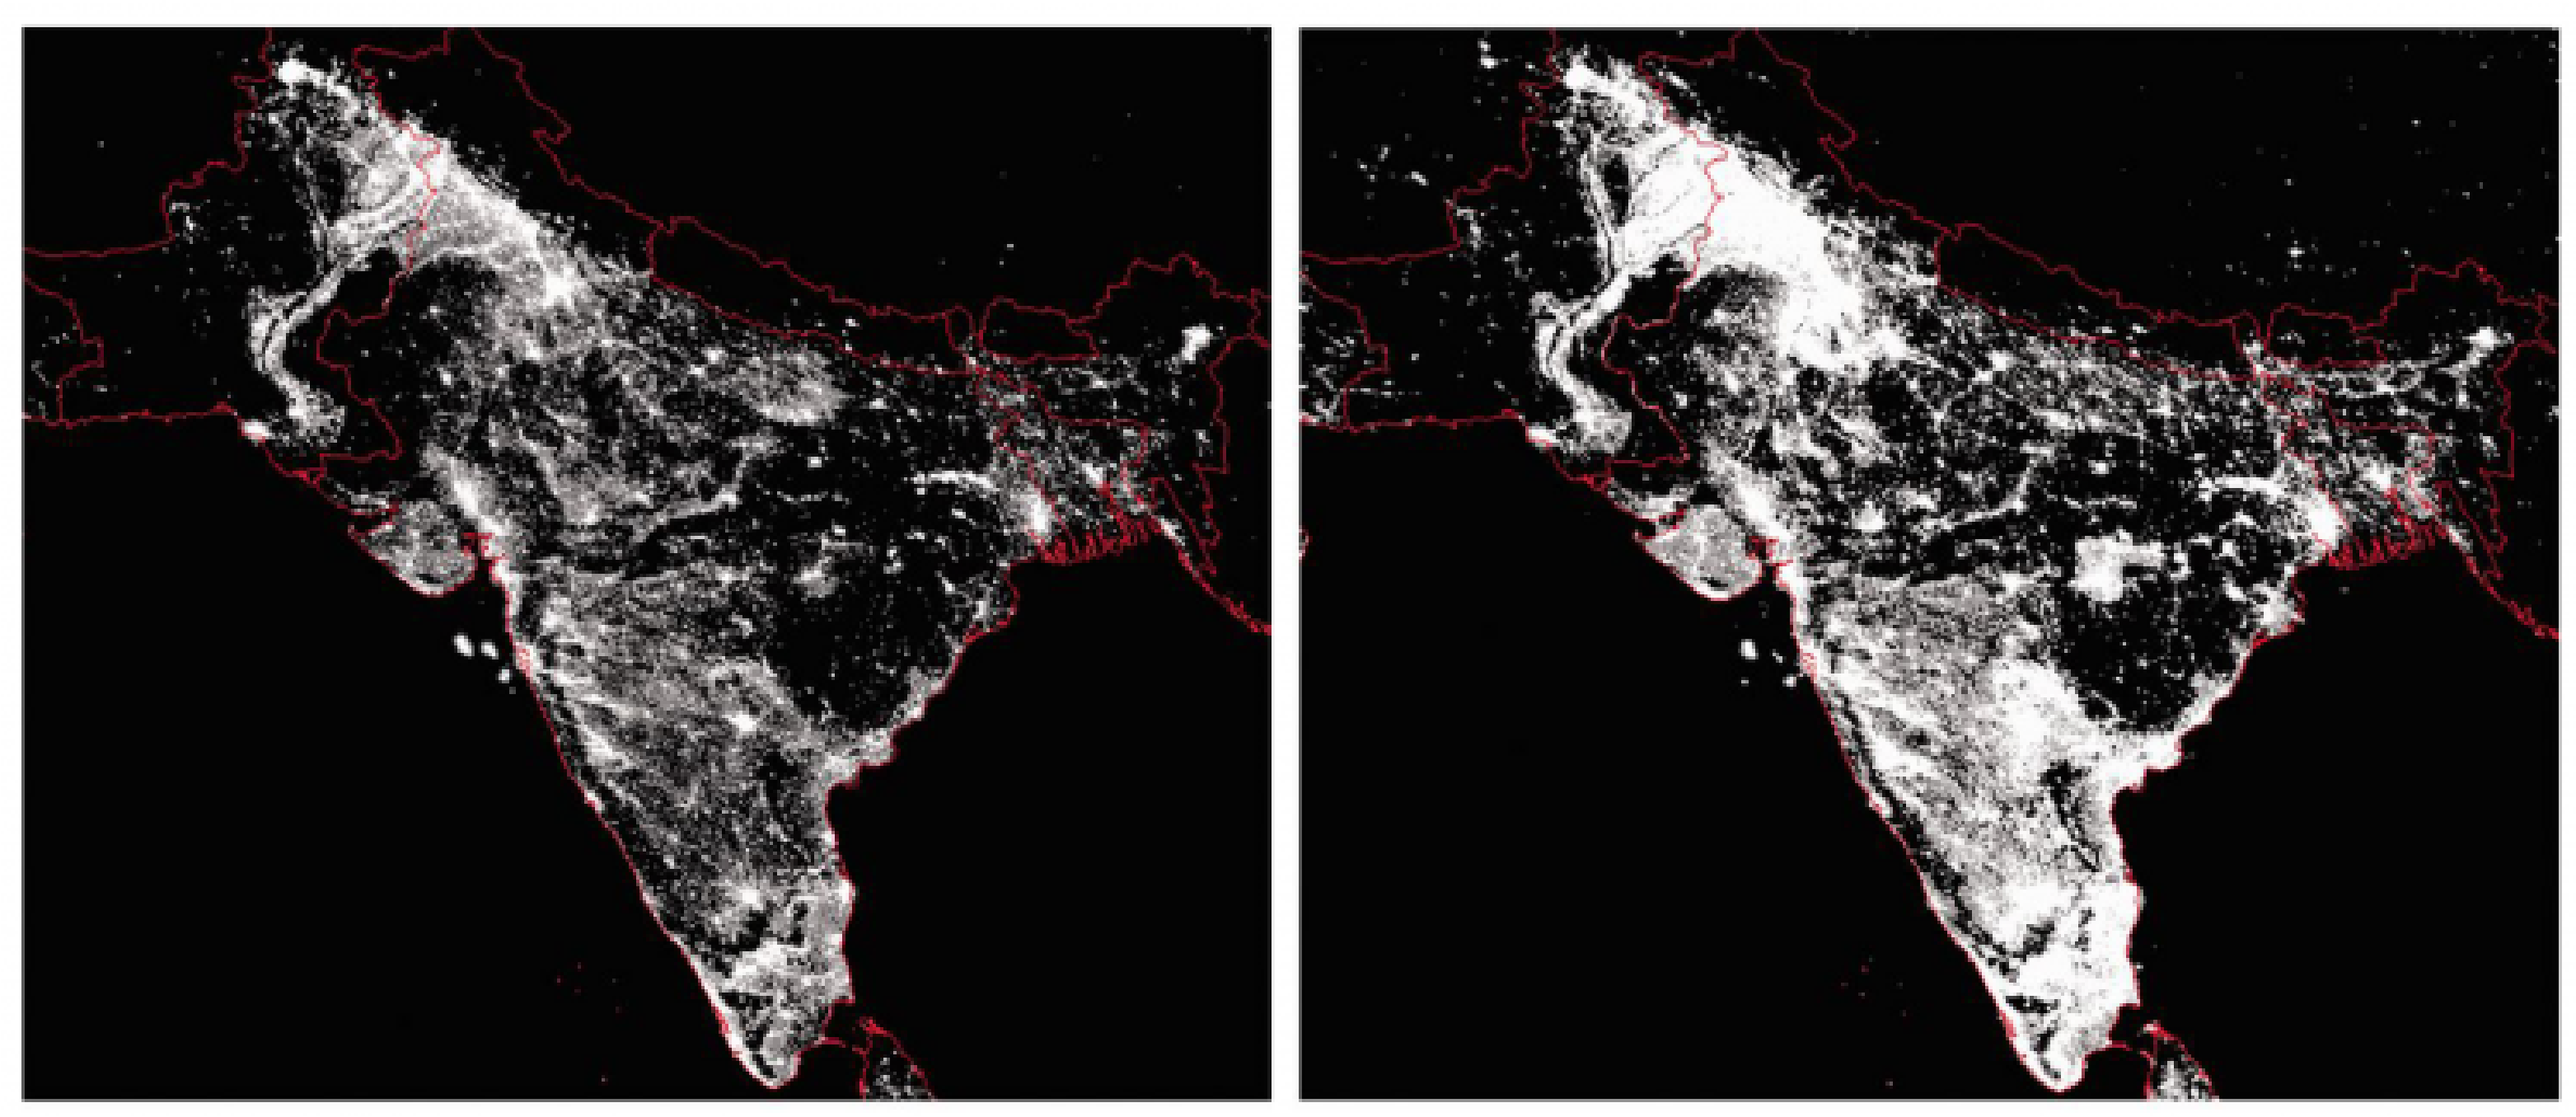
\includegraphics[width=0.6\linewidth]{/Users/alistairgj/Documents/GitHub/IoT_ResearchProject/IoT_November/images/satelliteImages} 

}

\caption{Satellite images of South Asia by night. Left (South Asia in 1994) Right (South Asia in 2010). Images are taken from Maxim Pinkovskiy and Xavier Sala-i-Martin (2016) - Lights, Camera ... Income! Illuminating the National Accounts-Household Surveys Debate. The Quarterly Journal of Economics.}\label{fig:satelliteImagesAsia}
\end{figure}

\begin{figure}[H]

{\centering 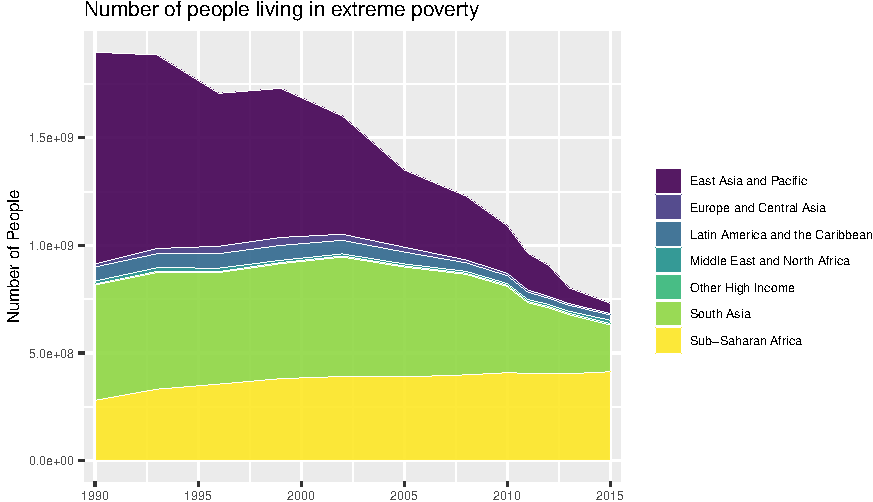
\includegraphics{MD_Final_files/figure-latex/globalPovertyPlot-1} 

}

\caption{The number of people living in extreme poverty between the years of 1990 till 2015, segmented by region. Source: The World Bank}\label{fig:globalPovertyPlot}
\end{figure}

\hypertarget{the-rise-and-rise-of-the-world-wide-web}{%
\subsubsection{The Rise and Rise of the World Wide
Web}\label{the-rise-and-rise-of-the-world-wide-web}}

According to the International Telecommunication Unions (\textbf{ITU})
2015 figures, Internet penetration has grown from just over 400 millions
users (6 per cent of global population) in 2000 to 3.2 billion users in
2015 (43 per cent of global population). This includes around 2 billion
users from developing countries
{[}\protect\hyperlink{ref-duttaGlobalInformationTechnology2015}{2}{]}.
ICTs bring a broad range of benefits and are recognised as a key to
eradicating poverty and unemployment. They enable and facilitate the
building of a people-centred, inclusive and development-oriented
Information Society, where everyone can create, access, utilise and
share information and knowledge. This enables individuals, communities
and peoples to achieve their full potential in promoting their
sustainable development and improving their quality of life
{[}\protect\hyperlink{ref-InformationCommunicationTechnologies}{3}{]}.
In addition to a rapidly growing internet user-base both in the
developing and developed world, the nature of internet usage has
fundamentally changed. Once the purview of academics, engineers and
computer scientists sending tiny packets of information back and forth,
there are now some 2.5 quintillion bytes of data created each day by all
manner of users, industries and sensors, to name a few
{[}\protect\hyperlink{ref-DataNeverSleeps}{4}{]}.

\begin{figure}[H]

{\centering 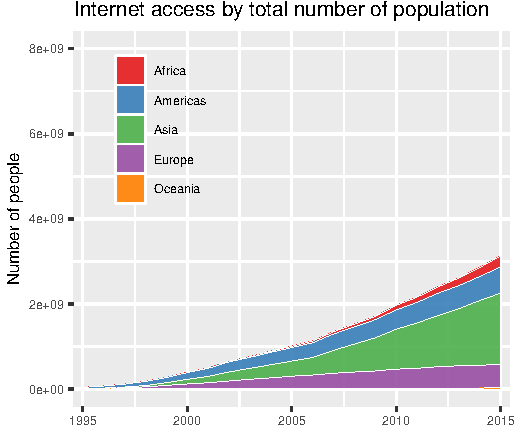
\includegraphics{MD_Final_files/figure-latex/internetAccessPlot-1} 

}

\caption{Internet access by total number of population, Source: The World Bank, World Development Indicators}\label{fig:internetAccessPlot}
\end{figure}

\hypertarget{forging-a-new-technological-paradigm}{%
\subsubsection{Forging a New Technological
Paradigm}\label{forging-a-new-technological-paradigm}}

Such rapid and widespread internet adoption has created a seemingly
insatiable demand for exponentially greater computational power and
digital storage capacity. This has led to a new and ubiquitous
technological paradigm: Cloud Computing. Cloud Computing is succinctly
defined as; the practice of using a network of remote servers hosted on
the Internet to store, manage, and process data, rather than a local
server or a personal computer
{[}\protect\hyperlink{ref-CloudComputingDefinition}{5}{]}.

As with the initial rise and widespread implementation of the Internet,
Cloud Computing itself acts as a facilitator for new technologies. One
such example being the Internet of Things (\textbf{IoT}) paradigm. The
IoT can be surmised as the extension of the Internet and the Web into
the physical realm, by means of the widespread deployment of spatially
distributed devices with embedded identification, sensing and/or
actuation capabilities, allowing objects to be sensed or controlled
remotely through the internet
{[}\protect\hyperlink{ref-danielemiorandiInternetThingsVision2012}{6}{]},
{[}\protect\hyperlink{ref-binghuangServiceOrientedComputing16th2018}{7}{]},
{[}\protect\hyperlink{ref-luigiatzoriInternetThingsSurvey2010}{8}{]}.
IoT thus represents a convergence of real-world objects and digital
objects into a unified cyber-physical system.

\hypertarget{the-bigger-picture}{%
\subsubsection{The Bigger Picture}\label{the-bigger-picture}}

Considering the bigger picture of societal benefit, as seen in Figure
\ref{fig:globalPovertyPlot}, from 1990 through 2015 the number of people
living in extreme poverty has dropped by more than half. As evidenced by
Figure \ref{fig:internetAccessPlot}, over the same time period, the
percentage of people with access to the internet has move from around 1
per cent to an average of around 50 per cent (this trend is now moving
exponentially as a function of time). And, Figure
\ref{fig:populationGrowthPlot} shows that over the last 100 years, the
human population has experienced unprecedented growth from 1 billion
individuals to in excess of 7 billion. Mankind have thus simultaneously
increased our population, increased of technological development and
decreased poverty (to name but a few, `key performance indicators').

\begin{figure}[H]

{\centering 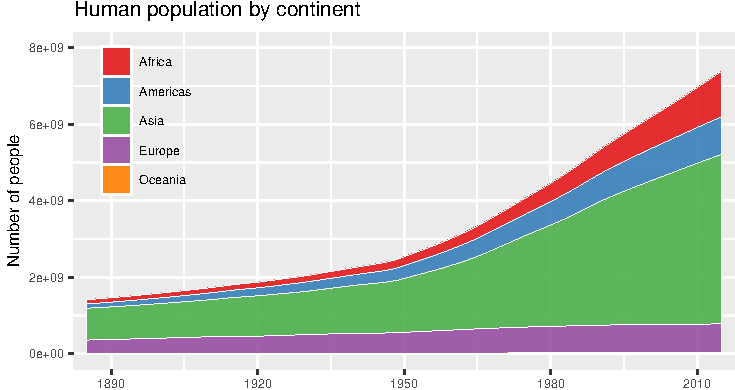
\includegraphics{MD_Final_files/figure-latex/populationGrowthPlot-1} 

}

\caption{Human population by continent, Source: The World Bank, World Development Indicators}\label{fig:populationGrowthPlot}
\end{figure}

The success of modern human society is not without consequence. All of
the benefits our society has enjoyed from the development, production
and deployment of technology, has required vast amounts of energy. This
energy has, since the industrial revolution, primarily been derived from
the burning of fossil fuels, as illustrated by Figure
\ref{fig:globalEnergyPlot}.

\begin{figure}[H]

{\centering 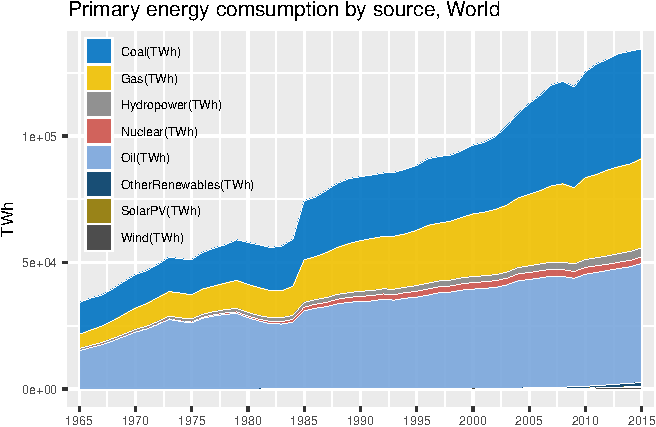
\includegraphics{MD_Final_files/figure-latex/globalEnergyPlot-1} 

}

\caption{Energy Production and Changing Energy Sources, Source: Our World in Data}\label{fig:globalEnergyPlot}
\end{figure}

The International Panel on Climate Change (IPCC) finds that Human
activities are estimated to have caused approximately 1.0°C of global
warming above pre-industrial levels, with a likely range of 0.8°C to
1.2°C. Global warming is likely to reach 1.5°C between 2030 and 2052 if
it continues to increase at the current rate
{[}\protect\hyperlink{ref-intergovernmentalpanelonclimatechangeGlobalWarming2018}{9}{]}.

Climate change poses an existential threat to modern human civilisation,
with warming of between 1.5°C and 2°C predicted to cause increases in
mean temperature in most land and ocean regions, hot extremes in most
inhabited regions and heavy precipitation changes in some regions.
Additionally, increases in ocean temperature as well as associated
increases in ocean acidity and decreases in ocean oxygen levels are
projected to reduce risks to marine biodiversity, fisheries, and
ecosystems, and their functions and services to humans. Taken together,
these effects will lead to risks of the health, livelihoods, food
security, water supply, human security, and economic growth
{[}\protect\hyperlink{ref-intergovernmentalpanelonclimatechangeGlobalWarming2018}{9}{]}.

\begin{figure}[H]

{\centering 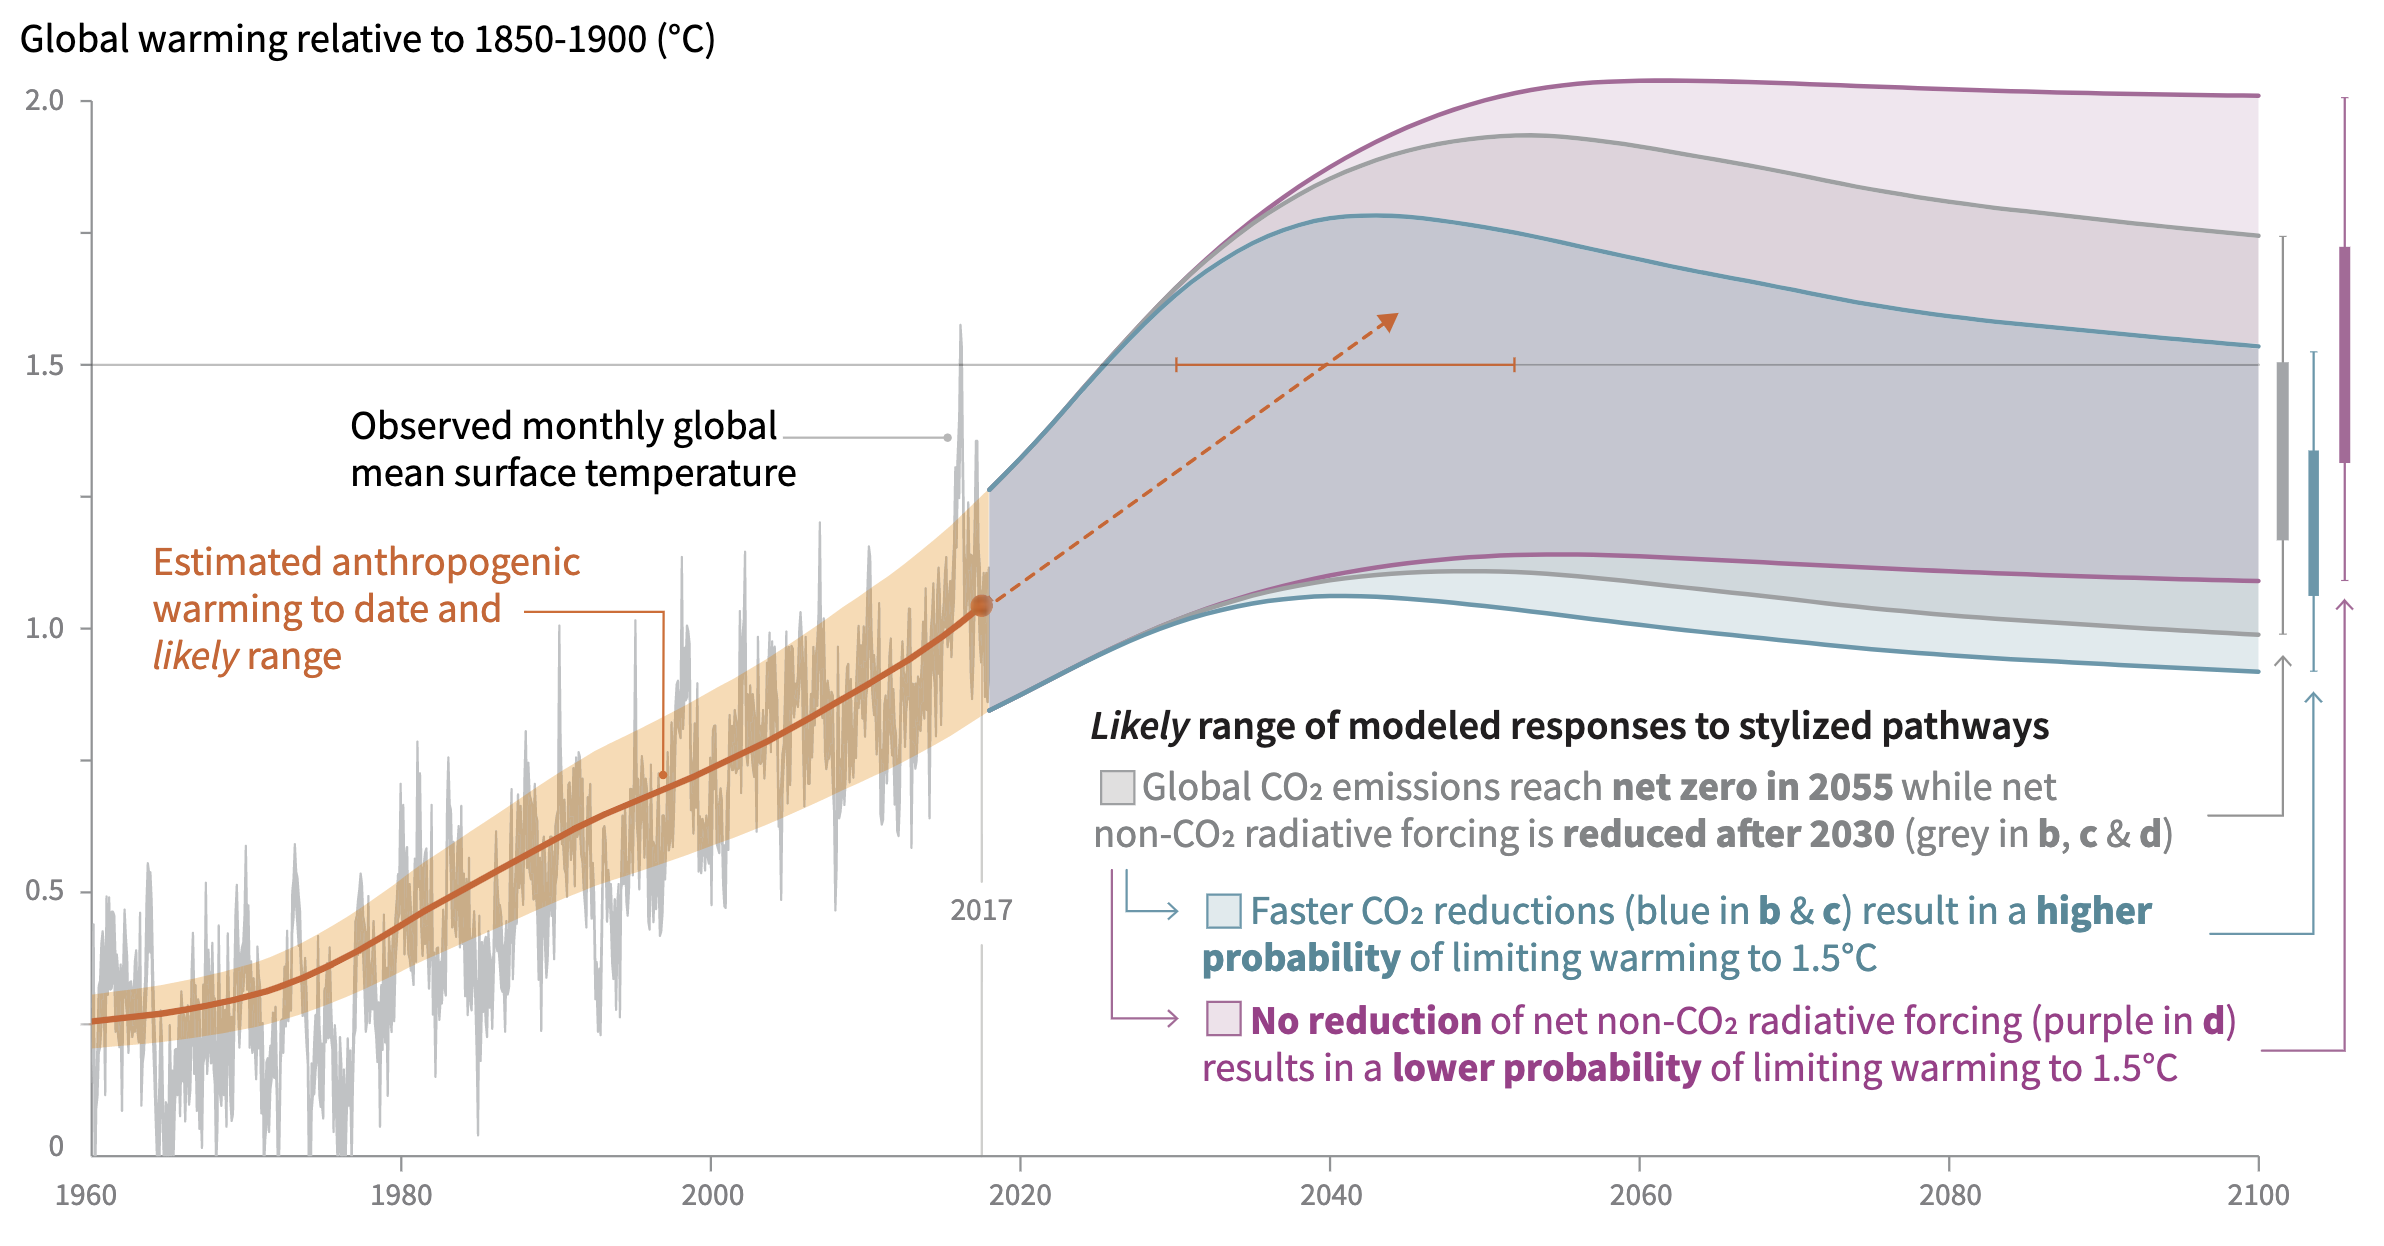
\includegraphics[width=0.8\linewidth]{/Users/alistairgj/Documents/GitHub/IoT_ResearchProject/IoT_November/images/warmingTrend} 

}

\caption{Atmospheric Changes with respect to Carbon Emissions and Global Warming - Observer and Projected. Source: Intergovernmental Panel on Climate Change, 2018}\label{fig:warmingTrend}
\end{figure}

It is therefore imperative moving forward as a species that all steps
are be taken to mitigate the emission of greenhouse gases and abate the
advance of anthropomorphic climate change. The scale of the challenge is
such that technology itself will prove critical in effectively combating
this existential threat to civilisation. When considering energy
consumption, the industrial sector (including the non-combusted use of
fuels) currently consumes around half of all global energy and feedstock
fuels, with residential and commercial buildings (29\%) and transport
(21\%) accounting for the remainder
{[}\protect\hyperlink{ref-EnergyDemandSector}{10}{]}

\begin{figure}[H]

{\centering 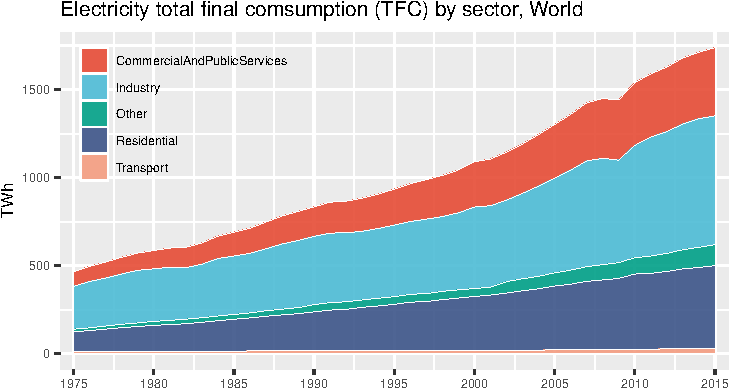
\includegraphics{MD_Final_files/figure-latex/sectorEnergyPlot-1} 

}

\caption{ADD TEXT}\label{fig:sectorEnergyPlot}
\end{figure}

\hypertarget{optimising-global-energy-usage}{%
\subsubsection{Optimising Global Energy
Usage}\label{optimising-global-energy-usage}}

Thus far, our staggering global achievements, including lifting hundreds
of millions out of poverty, rapid global technological deployment and
strong population growth has been inexorably linked to increased energy
consumption. This in turn has led to perturbations in atmospheric
chemistry, in the form of anthropogenic climate change (amongst many
other environmental challenges), which fundamentally threatens our
global achievements. It therefore stands that the key to continued human
prosperity is to de-couple growth in energy demand from economic growth.
In this work we will explore the possibility of reducing energy
consumption via the optimization of services to end users in an IoT
Smart Home.

\hypertarget{the-iot-smart-home-service-oriented-computing}{%
\subsubsection{The IoT Smart Home \& Service Oriented
Computing}\label{the-iot-smart-home-service-oriented-computing}}

As mentioned above, residential and commercial buildings account for
29\% of energy demand globally
{[}\protect\hyperlink{ref-Consumption}{11}{]}. In this work we propose
that an avenue for reduced energy consumption is the optimization of
existing services and utilities to end users in an IoT Smart Home. In
this proposed smart home, the daily activities of the end user can be
performed with the support of a personalised artificial intelligence
(AI) system, such that the timing and manner of energy intensive
activities is optimised to reduce overall energy consumption, whilst
still considering the level of convenience afforded to the end user.
This work uses sensor data analogous to what would be expected to be
produced from a sensor rich IoT smart home and considers the interplay
between end user convenience; predictive analytics; predictive service
offering; energy consumption; demand response and smart electricity
grids.

\hypertarget{aim}{%
\subsection{Aim}\label{aim}}

In this work we aim to use previously captured sensor data of domestic
activities to develop a framework for the consideration of convenience
with respect to energy savings. We will extrapolate these findings into
a proposed hypothetical scenario in which an end user occupying an IoT
smart home is able to use a smartphone application to personalise the
level of convenience, cost saving or energy saving.

\hypertarget{research-questions}{%
\subsubsection{Research Questions}\label{research-questions}}

\begin{enumerate}
\def\labelenumi{\arabic{enumi}.}
\tightlist
\item
  Can a generalised methodology for processing data pertaining to end
  user activity in a smarthome be developed?
\item
  Can historical sensor data be used to build a meaningful model for the
  relationship between end user convenience and cost?
\end{enumerate}

\hypertarget{preliminaries}{%
\section{Preliminaries}\label{preliminaries}}

Significant growth in digital interconnectivity over the last 20 years
has given the internet a pivotal role as an essential element of
economic growth
{[}\protect\hyperlink{ref-haseebDoesInformationCommunication2019}{12}{]}.
Cloud computing and the IoT paradigm has enabled the association of
previously disparate fields into a larger coherent framework. Namely,
smart home appliances, demand-response, energy consumption, predictive
analytics predictive service offering and end user convenience. This
work proposes a framework for the association of sensor data as an into
into a machine learning model as a means of predicting energy-intensive
appliance usage in a hypothetical IoT smarthome.

\hypertarget{related-work}{%
\subsection{Related Work}\label{related-work}}

\hypertarget{ubiquity-of-the-world-wide-web-and-implications-for-energy-consumption}{%
\subsubsection{Ubiquity of the World Wide Web and Implications for
Energy
Consumption}\label{ubiquity-of-the-world-wide-web-and-implications-for-energy-consumption}}

The International Telecommunication Union estimated about 3.2 billion
people, or almost half of the world's population, would be online by the
end of the 2015
{[}\protect\hyperlink{ref-InformationCommunicationTechnologies}{3}{]}.
The impact of internet usage and mobile cellular subscriptions
(\textbf{ICTs}), globalization, electricity consumption, financial
development, and economic growth on environmental quality has been
examined
{[}\protect\hyperlink{ref-haseebDoesInformationCommunication2019}{12}{]}.
By using 1994--2014 panel data of the Brazilian, Russian, Indian,
Chinese \& South African (\textbf{BRICS}) economies, empirical results
demonstrate that rise in both internet usage and mobile cellular
subscription ICTs likely mitigates CO2 emissions.

\hypertarget{smart-metering}{%
\subsubsection{Smart Metering}\label{smart-metering}}

A Smart meter is an electronic device that records consumption of
electric energy and communicates the information to the electricity
supplier for monitoring and billing. In the Unites States (for example)
smart meters are a significant part of the larger Smart Grid
infrastructure, and as far back as 2012, had been installed in over 25
million U.S. homes
{[}\protect\hyperlink{ref-hornePrivacyTechnologyNorms2015}{13}{]}. Smart
Meters transmit information about consumer electricity use to utility
companies at vastly shorter time intervals than before and this
information helps utility companies to coordinate power supply and
demand, detect outages, implement time-of-use and dynamic pricing, and
in other ways improve system efficiency and reliability. Additionally,
these data are also becoming increasingly available, and sought-after,
by end-users themselves. Indeed, the main purpose of provisioning smart
metering data to end users is to encourage the use of less electricity,
by better informing users of their consumption patterns
{[}\protect\hyperlink{ref-jui-shengchouCloudForecastingSystem2019}{14}{]}.
In the aggregate, these savings can significantly reduce national energy
use and curb energy emissions while addressing pressing geopolitical and
environmental concerns related to energy security and sustainability
{[}\protect\hyperlink{ref-graabSmartGridSmart2011}{15}{]}.

Since the widespread deployment of smart meter technology, there has
been huge interest in the capability of these technologies with respect
to the technical capacity of utility companies to manage demand (through
demand response programs), incorporate renewable sources of electricity
into the system, and increase the overall efficiency and reliability of
the system
{[}\protect\hyperlink{ref-hornePrivacyTechnologyNorms2015}{13}{]}.

\hypertarget{electricity-demand-response-smart-electricity-grids-and-smart-home-data}{%
\subsubsection{Electricity Demand Response, Smart Electricity Grids and
Smart Home
Data}\label{electricity-demand-response-smart-electricity-grids-and-smart-home-data}}

Predicting and influencing residential energy use has been the subject
to extensive study
{[}\protect\hyperlink{ref-ilzelaicaneEvaluationHouseholdElectricity2015}{16}{]}.
Literature indicates that factors such as occupant behaviour and
socio-economic status are important. For example Nielsen attributed 36\%
of variation in energy consumption of homes to lifestyle and occupant
behaviour, and 64\% to socio-economic influences. This is exemplified by
the work of De et al, who show that in developing nations, cooking
consumes up to 90\% of the overall residential energy consumption and is
mainly based on non-renewable energy
{[}\protect\hyperlink{ref-d.m.murrayApplianceElectricalConsumption2018}{17}{]}.
Other factors such as climate zone, number of occupants, income level,
age of home, and size of home have also been correlated with home energy
use
{[}\protect\hyperlink{ref-ilzelaicaneEvaluationHouseholdElectricity2015}{16}{]}.
There has been much work both on using smart meter data to evaluate
consumer behaviour, and the interplay between smart appliances and
shifting households' electricity demand.

Kavousian et al identify the need for developing an analytical method
that can leverage 15-minute or 30-minute interval energy consumption
data produced via smart metering in order to improve the effectiveness
of energy efficiency programs. They note that utilities spend millions
of dollars annually to improve appliance energy efficiency. By way of
example, in 2013 utilities in California US spent \$80 M USD on
appliance and plug load efficiency programs, the highest expenditure
among all utility energy efficiency programs
{[}\protect\hyperlink{ref-amirkavousianRankingApplianceEnergy2015}{18}{]}.
A need for analytical methodologies that can process smart meter data
and allow energy reduction savings to be identified is demonstrated.
Using a smart meter dataset of 4231 households, containing information
on electricity consumption at 30-minute intervals, with aggregated local
weather data, the authors use smart meter data to rank residential
appliance efficiency. Various control methodologies are embedded into
the analytical process, taking into account building type, building size
(e.g., apartment, detached), household type (e.g., de facto, single,
dependents), respondent age and heater type (e.g., electric or gas). The
data set included 120+ household variables, many of which were highly
correlated, model selection techniques were used to successfully reduce
dimensionality. A set of load profiles were compiled based on the
results (where normalized load was plotted as a function of hour of
day). It was determined that household behaviour and demographic can be
used to generate positive and negative energy efficiency coefficients
with respect to load profiles. This work has implications for energy
grid planning -- for example in high-density housing versus suburban
housing.

Karjalainen considers the manner in which smart meter data is
communicated to end users, with the principal purpose of the paper being
to study what kind of electricity consumption feedback consumers
understand and prefer
{[}\protect\hyperlink{ref-karjalainenConsumerPreferencesFeedback2011}{19}{]}.
It is noted that the most effective feedback tools for engaging
households in reducing energy consumption are both computerized and
interactive. In this work a series of options for feedback is gathered,
for example consumption (kHh), power (W), cost (\$), environmental
impact (e.g., kg CO2), total for household, disaggregation by appliance,
real time, hour, day, and so on. Examples of feedback options are shown
in Figure \ref{fig:fb1} and Figure \ref{fig:fb2}, below.

\begin{figure}[H]

{\centering 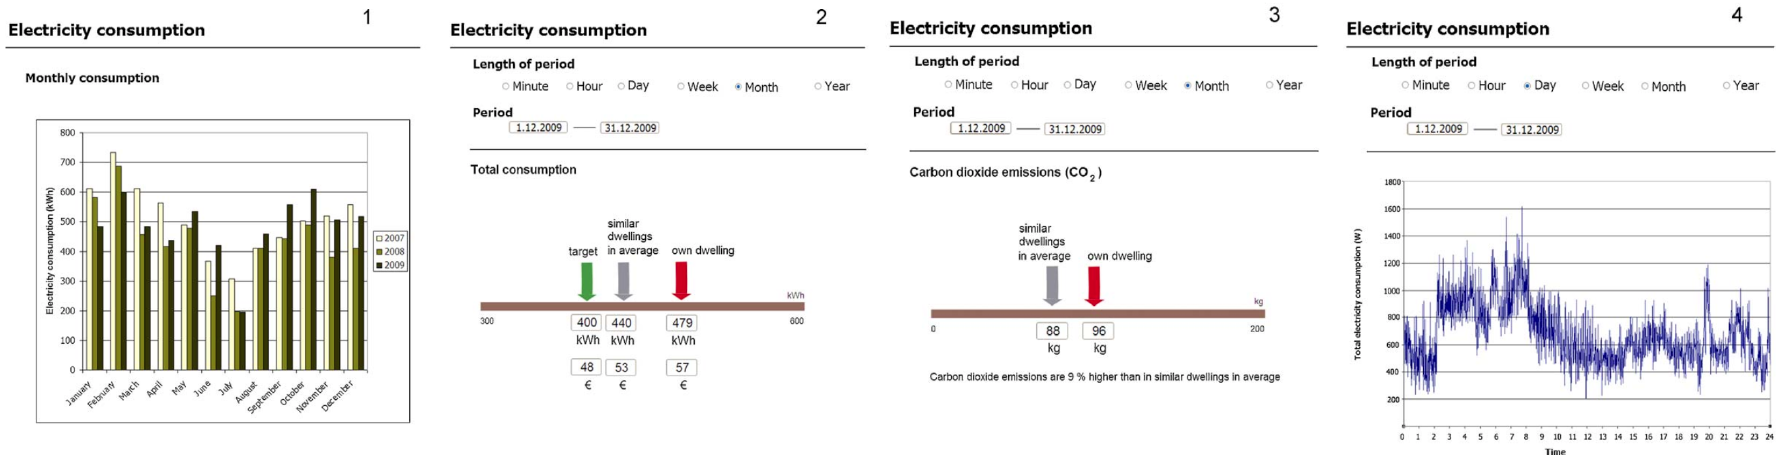
\includegraphics[width=1\linewidth]{/Users/alistairgj/Documents/GitHub/IoT_ResearchProject/IoT_November/images/dash1234} 

}

\caption{Option One, Two, Three and Four of the smart meter data dashboards proposed by Karjalainen}\label{fig:fb1}
\end{figure}

\begin{figure}[H]

{\centering 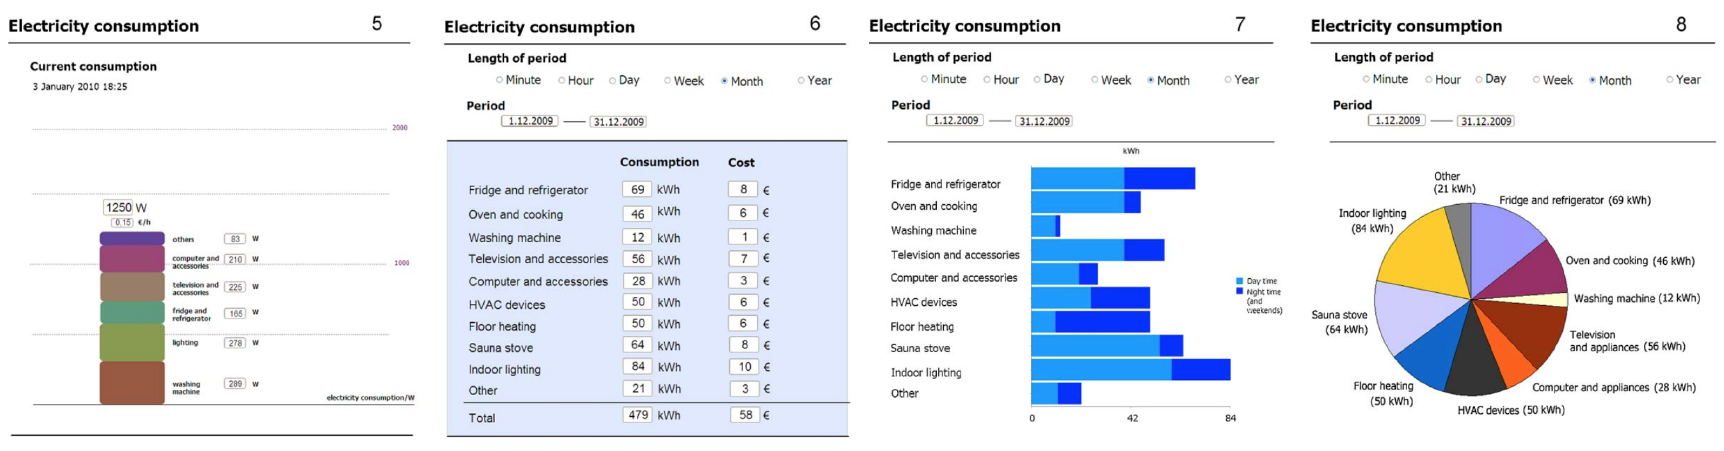
\includegraphics[width=1\linewidth]{/Users/alistairgj/Documents/GitHub/IoT_ResearchProject/IoT_November/images/dash5678} 

}

\caption{Option Five, Six, Seven and Eight of the smart meter data dashboards proposed by Karjalainen}\label{fig:fb2}
\end{figure}

The results of qualitative participant interviews clearly showed that
while some consumers are very interested in saving household
electricity, other consumers show only a little interest. When
specifically asked to list what measures (if any) were typically taken
at home to realize reductions in energy usage, some respondents listed
numerous measures, while others just said they turn lights off in rooms
that are empty. The author also found some participants were unaware of
differences in stand-by versus active modes of operation for electrical
appliances, resulting in practising inefficient energy saving measures
in the home environment. When trialling feedback prototypes to
participants, two main issues were encountered: (1) many people are not
familiar with scientific units and do not understand the difference
between W and kWh and (2) many people do not understand how carbon
dioxide emissions are related to electricity consumption. It is perhaps
surprising that the overall most popular prototype was `6', below.
Perhaps because unlike the other prototypes, this clearly (the most
clearly) articulates cost. The concept of convenience was absent
entirely from consideration.

In the domain of supply and demand economics, consumer behaviour and
smart appliances Kobus et al investigated if households can shift their
electricity demand to times when electricity is abundantly available
{[}\protect\hyperlink{ref-charlotteb.a.kobusReallifeAssessmentEffect2015}{20}{]}.
Using a household electrical monitoring system (\textbf{EMS}) coupled to
a smart appliance (smart washing machine), photovoltaic cells and the
electricity grid, they were able to show that households can shift
10--77\% of the electricity demand of their washing machine. This
longitudinal study was conducted via the participation of 50 Dutch
households over a period of one year. By utilizing an EMS which shows
appliance status, dynamic tariff information and current status of
household electricity usage, participants are able to schedule smart
washing machine use in such a way that cost is minimized.

\begin{figure}[H]

{\centering 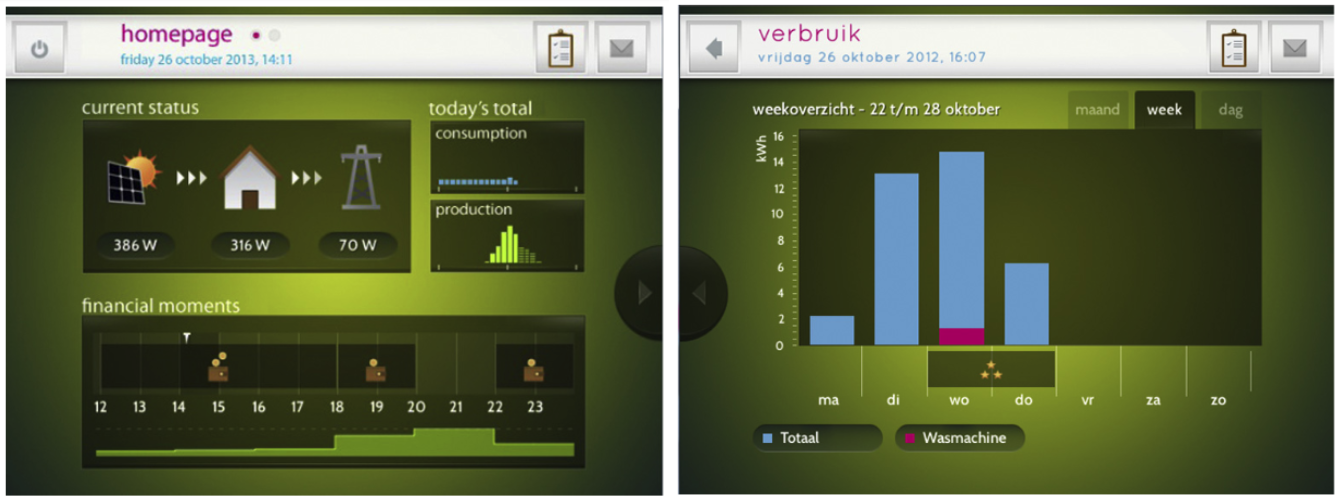
\includegraphics[width=0.6\linewidth]{/Users/alistairgj/Documents/GitHub/IoT_ResearchProject/IoT_November/images/kobusDash} 

}

\caption{Example dashboards proposed by Kobus et al}\label{fig:unnamed-chunk-1}
\end{figure}

Their work is in response to two major challenges to domestic
electricity supply and demand. The first being the amount of distributed
renewable electricity generation is increasing with time (e.g., as more
households install photovoltaic (\textbf{PV}) panels), and the second
that electricity demand will continue to significantly increase moving
into the foreseeable future. These developments pose great challenges to
`traditional' power systems, where supply follows demand entirely. Smart
grids are proposed as a potential solution for the affordable
introduction of cleaner electricity producing and consuming
technologies.

Cetin et al consider electricity usage of appliance, as when aggregated,
this accounts for approximately 30 per cent of electricity used in the
residential building sector
{[}\protect\hyperlink{ref-k.s.cetinApplianceDailyEnergy2014}{21}{]}.
This, together with small appliances, home electronics and lighting,
account for more than 2/3 of total residential electricity use. Cetin et
al also highlight that influencing `time of use' is becoming
increasingly important to control the stress on today's electrical grid
infrastructure. The authors seek to determine when refrigerators,
clothes washers, clothes dryers and dishwashers are predominantly used
(and thus consume energy) and what causes variation in their use. Using
disaggregated energy data from 40 homes over a period of 1-year,
normalized load profiles for the four target appliances were generated,
as a percentage of daily electricity load.

\begin{figure}[H]

{\centering 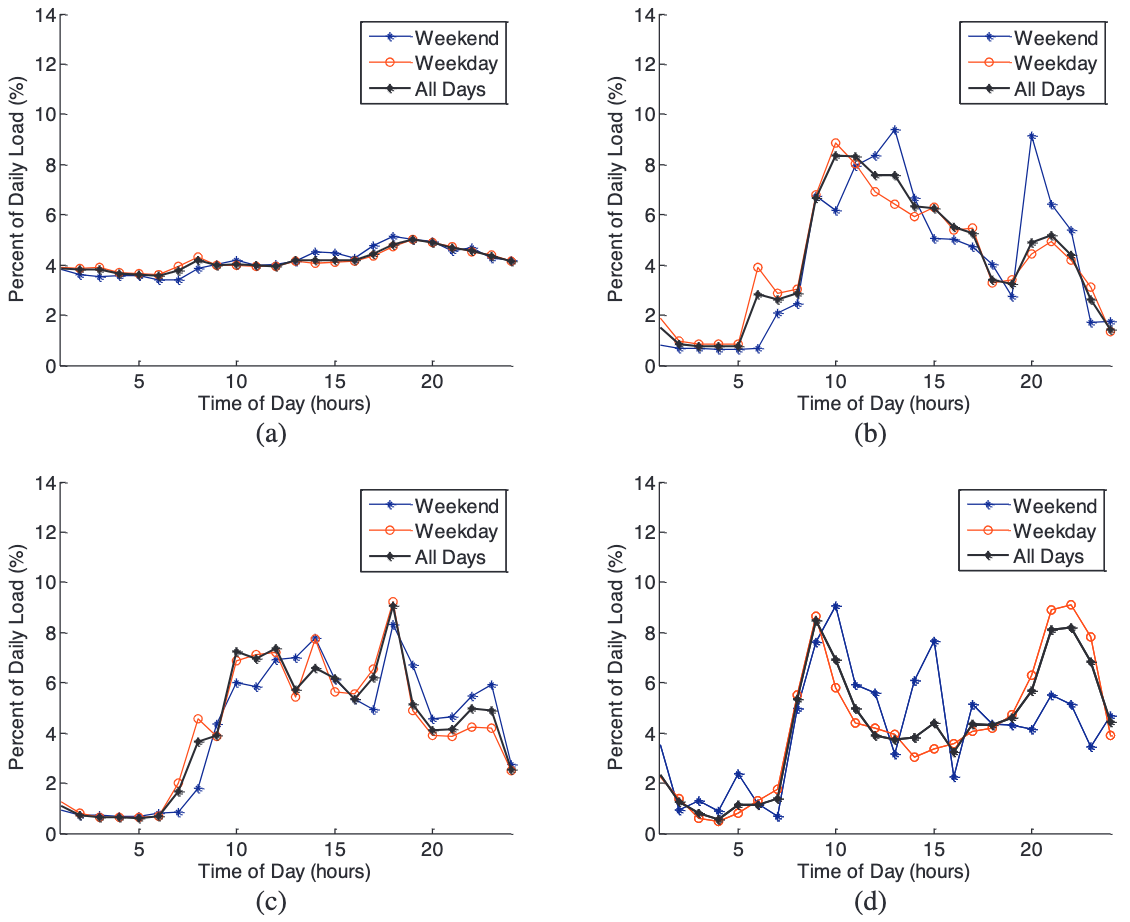
\includegraphics[width=0.65\linewidth]{/Users/alistairgj/Documents/GitHub/IoT_ResearchProject/IoT_November/images/cetinResults} 

}

\caption{Appliance energy consumption with respect to time of day, A = refrigerators, B = cloths washers, C = Cloths dryers and D = Dishwashers}\label{fig:unnamed-chunk-2}
\end{figure}

It was found that the refrigerator had the most consistent consumption
profile across all homes surveyed. Influencing factors for the
refrigerator were correlated to both indoor and outdoor temperature,
however effect was found to be minimal. The clothes washer and dryer
were found to have the greatest variation in normalised energy use by
hour, with the greatest period of use from 9am until 2pm. The dishwasher
had distinct peaks in load profile at 9am and 10pm. The authors found
that user-dependent appliance use patterns vary more between homes and
between days than automated appliances, weekday and weekend use patterns
of appliances are similar, and that electricity use varies more between
houses during peak use times of day than during low-use times. Murray et
al further explore the topic of home appliance energy consumption using
smart meter data, specifically pertaining to residential activities
around food storage and preparation
{[}\protect\hyperlink{ref-d.m.murrayApplianceElectricalConsumption2018}{17}{]},
with the aim of providing a model that can easily be applied to existing
smart meter energy datasets. The authors use real-time energy
consumption data from microwaves and ovens, from which user behaviour /
desired outcome can be implicitly associated (for example, oven usage on
a weekday between the hours of 6pm and 8pm can be associated with the
behaviour of preparing dinner). Accurate energy consumption models for
major cooking appliances are successfully constructed, further
re-enforcing the value and widespread applicability of residential smart
meter data.

\hypertarget{predictive-modelling-and-forecasting}{%
\subsubsection{Predictive Modelling and
Forecasting}\label{predictive-modelling-and-forecasting}}

In the domestic predictive energy consumption space Basu et al consider
home automation systems linked via a communication network to enable
interaction, data collation and control of appliances remotely by end
users
{[}\protect\hyperlink{ref-kaustavbasuApplianceUsagePrediction2012}{22}{]}.
The potential competing priorities of energy savings versus comfort
optimization for home occupants is discussed. The objective of this work
is to propose a learning system that is able to help the home automation
system compute an energetic plan that is also satisfactory to user
requests. Taking into account correlation between appliances, a
time-series based multi-label classifier is used to predict appliance
usage up to one hour into the future.

The attribute construction technique of Knowledge Extraction applied.
This process aims to extract novel attributes from underlying
substructures in the training instances in the form of sub-events, for
example periodicity in data. This Knowledge Extraction process is
similar to the implicit associations used by Murray et al, in the
analysis of energy consumption for food preparation
{[}\protect\hyperlink{ref-d.m.murrayApplianceElectricalConsumption2018}{17}{]}.
The substructures are then fed to a propositional learner. The proposed
model is trained in an iterative manner and attempts to take into
account all the possible information based on consumption data, time of
the event and meteorological information. Time is specifically model
time as a periodic variable, segmenting on hour of day and day of week,
noting that this takes into account the periodic nature of human
behaviour. Using BR1, LP, CC1, CC2 and MLk machine learning algorithms,
the precision, recall and accuracy for a variety of
electricity-consuming appliances is determined (where each appliance
constitutes a target variable over a set of iterations). In the
evaluation phase they find that user behaviour toward an appliance is
highly variable and the predictability of an appliance is dependent on
the regularity of usage patterns of the inhabitants. It is specifically
noted that it is therefore very difficult for now to propose a generic
methodology of appliance prediction for private houses.

\begin{figure}[H]

{\centering 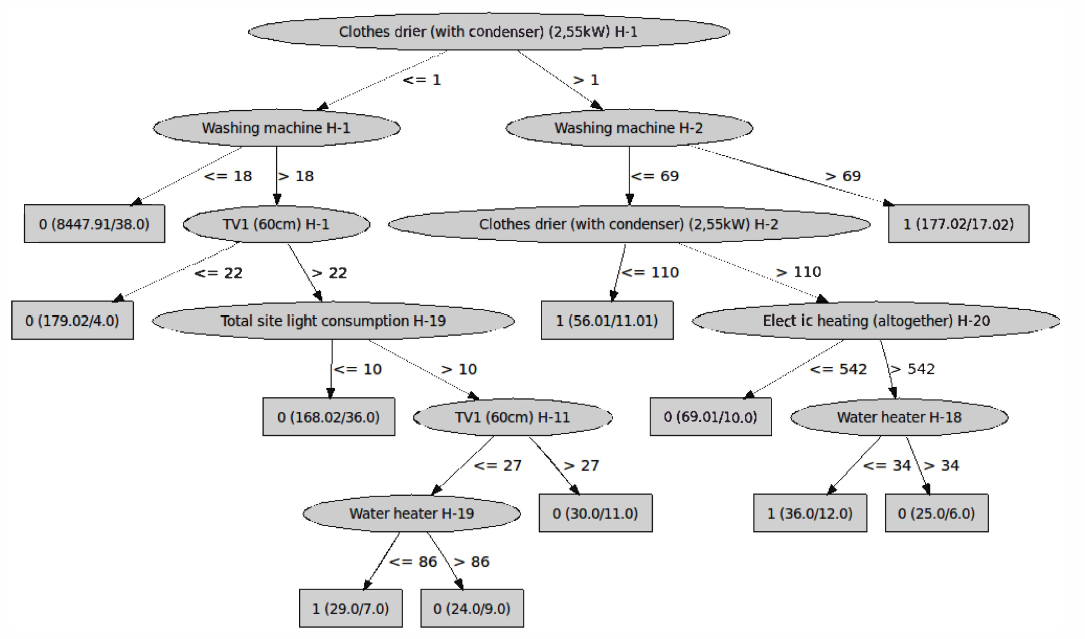
\includegraphics[width=0.8\linewidth]{/Users/alistairgj/Documents/GitHub/IoT_ResearchProject/IoT_November/images/basuTree} 

}

\caption{A decision tree from the work of Basu et al}\label{fig:unnamed-chunk-3}
\end{figure}

Chou et al consider global energy consumption in the residential housing
sector in the context of domestic energy information system (EIS) and
smart meter system (smart grids) technologies
{[}\protect\hyperlink{ref-jui-shengchouCloudForecastingSystem2019}{14}{]}.
They note two influential factors on overall residential energy
consumption, the first being the type and number of electrical
appliances and the second being the usage of these appliances by
occupants. It is proposed that a major challenge for people who are
willing to save energy at home is a lack of information about their
energy consumption. To test this hypothesis, the authors develop a
web-based energy information management system for the power consumption
of home appliances that monitors the energy load of a home, analyses its
energy consumption based on machine learning, and then sends information
to various stakeholders. Interaction with end-users in the home is
achieved via energy dashboards and emails. The authors propose that
end-users of this system can use forecast information and anomalous data
to enhance the efficiency of energy usage in their buildings especially
during peak times by adjusting the operating schedule of their
appliances and electrical equipment.

During this study, an EIS with 5 main components was installed in an
experimental building. The parts were as follows; (1) the internal
communication network, (2) the data management infrastructure, (3) the
automated prediction system, (4) the web-based system and dashboard and
(5) the early warning system. Data from both the smart meter and from
sensors was used to compile the model, including timestamps (YYYY-MM-DD
hh:mm:ss), outdoor temperature (ºC), total building energy consumption
(kWh), aggregated energy consumption data (e.g., second floor lighting)
and individual appliances. The backend of the application was notably
cloud-hosted. They found improve consumer satisfaction by providing
real-time services that enable end-users to monitor the energy
consumption easily.

\hypertarget{iot-and-end-user-convenience}{%
\subsubsection{IoT and End User
Convenience}\label{iot-and-end-user-convenience}}

The term Internet-of-Things (\textbf{IoT}) is used as an umbrella
keyword for covering various aspects related to the extension of the
Internet and the Web into the physical realm, by means of the widespread
deployment of spatially distributed devices with embedded
identification, sensing and/or actuation capabilities
{[}\protect\hyperlink{ref-danielemiorandiInternetThingsVision2012}{6}{]}.
The IoT paradigm is fundamental to this work, representing the
confluence of multiple technological advancements
{[}\protect\hyperlink{ref-luigiatzoriInternetThingsSurvey2010}{8}{]}
including, ubiquity of internet access, the availability of
high-performance internet connectivity, inexpensive consumer electronics
with embedded sensing and control systems, automation, real-time
analytics, machine learning, commodity sensors and embedded systems. In
the IoT paradigm, digital and physical entities can be linked, by means
of appropriate information and communication technologies, to enable a
whole new class of applications and services
{[}\protect\hyperlink{ref-danielemiorandiInternetThingsVision2012}{6}{]}.
One consequence resulting from the widespread deployment of consumer
electronics with IoT capability is the evolution of the Internet from
interconnecting computers to interconnecting things. Figure
\ref{fig:diagram}, below, represents the availability of services
provisioned by new means facilitated by the internet and cloud
computing.

\begin{figure}[H]

{\centering 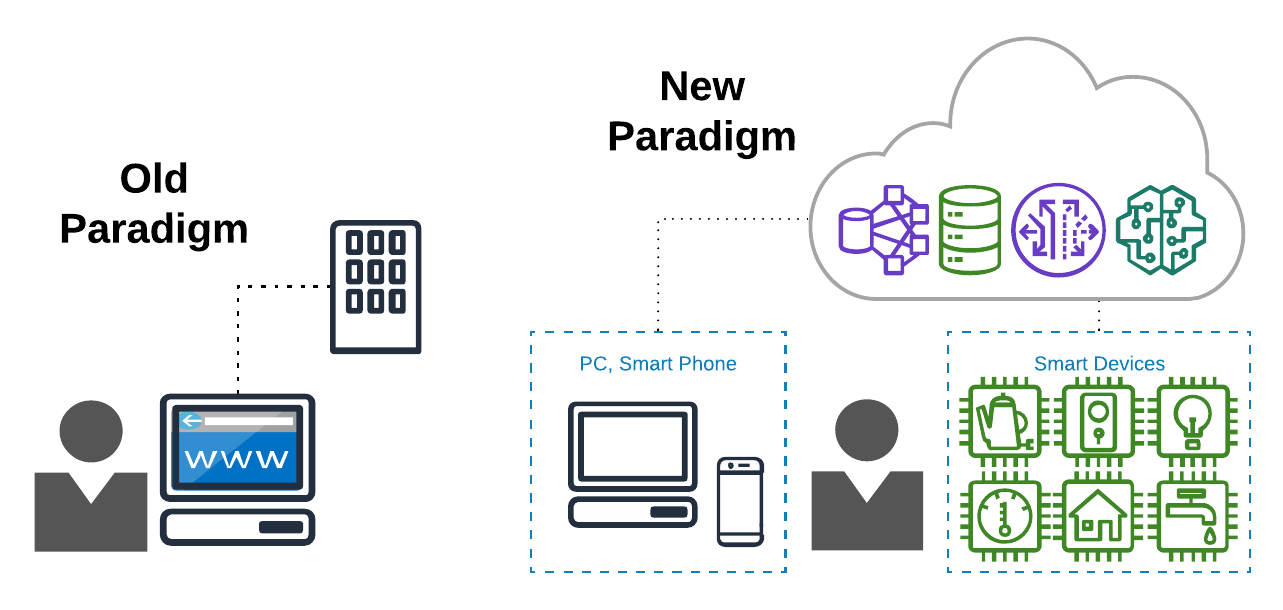
\includegraphics[width=0.65\linewidth]{/Users/alistairgj/Documents/GitHub/IoT_ResearchProject/IoT_November/images/oldNewParadigm} 

}

\caption{The old and new paradigms of end user interaction with the internet}\label{fig:diagram}
\end{figure}

Huang et al propose a novel service mining framework to personalize
services in an IoT-based smart home
{[}\protect\hyperlink{ref-binghuangServiceOrientedComputing16th2018}{7}{]}.
This work considers the notion of personal `convenience' as a driving
force behind the provisioning of services to end users. That is, in an
IoT smart home, where everything is interconnect, can services (for
example, the switching on or off of a light) be automatically served to
users such that their level of effort (to interact with their
surroundings) will be diminished, and thus their level of convenience
will be increased? The input for this work was data from domestic IoT
services, with a corresponding timestamp. The end user in this scenario
performs daily activities by interacting with IoT services, these
interactions are recorded as IoT service event sequences. The output for
this work was an IoT service model and a composite IoT service model
(based on spatio-temporal features).

\hypertarget{the-data-set}{%
\subsection{The Data Set}\label{the-data-set}}

The datasets were created during the thesis \emph{Activity Recognition
with End-User Sensor Installation in the Home} by Randy Joseph
Rockinson, Submitted to the Program of Media Arts and Sciences, School
of Architecture and Planning, in partial fulfilment of the requirement
for the degree of Master of Science in Media Arts and Sciences at the
Massachusetts Institute of Technology (MIT) February 2008
{[}\protect\hyperlink{ref-rockinsonActivityRecognitionHome}{23}{]}.

The aim of Rockinson was to considered the effect of end user versus
professional installation of a sensor array in the home - on the basis
that, if installation of sensors is to be considered as a high initial
cost, and a barrier to entry for end users wanting this technology, is
there a difference if a professional versus an end user performs the
installation? Between 80-100 reed switch sensors where installed in two
single-person apartments collecting data about human activity for two
weeks. The sensors were installed in everyday objects such as drawers,
refrigerators, containers, etc to record for example opening-closing
events (activation deactivation events) as the subject carried out
everyday activities.

\begin{figure}[H]

{\centering 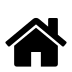
\includegraphics[width=1\linewidth]{/Users/alistairgj/Documents/GitHub/IoT_ResearchProject/IoT_November/images/home} 

}

\caption{The floor plan of the MIT home lab with a selection of sensors. Sensors in red correspond to those that require an energy source, while blue are activities that require only energy input from the end user, for example opening a door}\label{fig:unnamed-chunk-4}
\end{figure}

\pagebreak

\hypertarget{data-preprocessing-visualisation}{%
\section{Data Preprocessing \&
Visualisation}\label{data-preprocessing-visualisation}}

\hypertarget{importing-preprocessing-the-activities-meta-data}{%
\subsection{Importing \& Preprocessing the Activities Meta
Data}\label{importing-preprocessing-the-activities-meta-data}}

The dataset \texttt{S1Activities.csv} was imported into the interactive
development environment. These data contains a tabulated summary of
Heading, Category, Subcategory and a corresponding unique code. After
importation, the dataset has dimensionality of {[}3, 33{]}, with
\texttt{Heading}, \texttt{Category} \& \texttt{Subcategory} present as
non-null objects, as seen in Table \ref{tab:TAB_S1ActivitiesData} below.
The attribute \texttt{Code} (which codefies the unique set of Heading,
Category \& Subcategory) was imported as an index value (n=33). At this
time, the activities data will be kept in it's native state and will not
be subject to preprocessing.

\rowcolors{2}{gray!6}{white}
\begin{table}[!h]

\caption{\label{tab:TAB_S1ActivitiesData}The S1 activities dataset}
\centering
\fontsize{8}{10}\selectfont
\begin{tabular}[t]{llll}
\hiderowcolors
\toprule
  & Heading & Category & Subcategory\\
\midrule
\showrowcolors
1 & Employment related & Employment work at home & Work at home\\
5 & Employment related & Travel employment & Going out to work\\
10 & Personal needs & Eating & Eating\\
15 & Personal needs & Personal hygiene & Toileting\\
20 & Personal needs & Personal hygiene & Bathing\\
\bottomrule
\end{tabular}
\end{table}
\rowcolors{2}{white}{white}

\hypertarget{importing-preprocessing-the-sensor-meta-data}{%
\subsection{Importing \& Preprocessing the Sensor Meta
Data}\label{importing-preprocessing-the-sensor-meta-data}}

The dataset \texttt{S1sensors.csv} was imported into the interactive
development environment. These data contains a tabulated values for
Sensor ID, Room and Sensor Descriptor (e.g., light switch), with no
header row present in the original dataset. After importation, the
dataset has dimensionality of {[}3, 76{]}, with header 0, 1 \& 2
corresponding to SensorID, Room \& Sensor Descriptor, respectively, as
seen in Table \ref{tab:TAB_sensorData}. As all attributes are nominal,
they were imported as String data types.

\rowcolors{2}{gray!6}{white}
\begin{table}[!h]

\caption{\label{tab:TAB_sensorData}The S1 sensor meta data}
\centering
\fontsize{8}{10}\selectfont
\begin{tabular}[t]{lll}
\hiderowcolors
\toprule
0 & 1 & 2\\
\midrule
\showrowcolors
100 & Bathroom & Toilet Flush\\
101 & Bathroom & Light switch\\
104 & Foyer & Light switch\\
105 & Kitchen & Light switch\\
106 & Kitchen & Burner\\
\bottomrule
\end{tabular}
\end{table}
\rowcolors{2}{white}{white}

After importation these data were checked for duplicate values. The
\texttt{Sensor\ ID} attribute had a 76 unique values, the \texttt{Room}
attribute had only 7 unique values and the \texttt{Activity} attribute
had 28 unique values. Examples of the degeneracy in these attributes can
be seen in Table \ref{tab:TAB_sensorData}, e.g., Bathroom \& Light
Switch. Room{[}1{]} and Activity{[}2{]} were stripped of whitespace,
coerced to lowercase and concatenated using an underscore. The
concatenated vector was then bound to the dataframe and the column names
updated, resulting in \ref{tab:TAB_sensorDataProcessed}, below.

\rowcolors{2}{gray!6}{white}
\begin{table}[!h]

\caption{\label{tab:TAB_sensorDataProcessed}The first iteration of processed S1 sensor meta data}
\centering
\fontsize{8}{10}\selectfont
\begin{tabular}[t]{llll}
\hiderowcolors
\toprule
subActNum & room & activity & concat\\
\midrule
\showrowcolors
100 & Bathroom & Toilet Flush & bathroom\_toiletflush\\
101 & Bathroom & Light switch & bathroom\_lightswitch\\
104 & Foyer & Light switch & foyer\_lightswitch\\
105 & Kitchen & Light switch & kitchen\_lightswitch\\
106 & Kitchen & Burner & kitchen\_burner\\
\addlinespace
107 & Living room & Light switch & livingroom\_lightswitch\\
\bottomrule
\end{tabular}
\end{table}
\rowcolors{2}{white}{white}

The number of unique values in \texttt{dsS1Sensors.subActNum} is checked
once more and found to be n=76, indicating no degeneracy in this
attribute. The number of unique values in \texttt{dsS1Sensors.concat} is
found to be n=41, indicating the presence of degeneracy. This was
investigated by aggregating the duplicate attributes, which are
summarised in Table \ref{tab:TAB_numDupes}, below.
\rowcolors{2}{gray!6}{white}

\begin{table}[!h]

\caption{\label{tab:TAB_numDupes}Summary of the number of degenerate values (n) for each subactivity, where applicable.}
\centering
\fontsize{8}{10}\selectfont
\begin{tabular}[t]{rl}
\hiderowcolors
\toprule
n & concat\\
\midrule
\showrowcolors
3 & kitchen\_lightswitch\\
4 & kitchen\_burner\\
2 & livingroom\_lightswitch\\
7 & kitchen\_drawer\\
3 & kitchen\_refrigerator\\
\addlinespace
15 & kitchen\_cabinet\\
2 & kitchen\_door\\
5 & bedroom\_drawer\\
2 & bathroom\_medicinecabinet\\
2 & bathroom\_cabinet\\
\bottomrule
\end{tabular}
\end{table}
\rowcolors{2}{white}{white}

Referering to the work of Rockinson (from where the data originated) it
is was determined that these duplicate values are theresult of multiple
sensors with extremely similar functionality
{[}\protect\hyperlink{ref-rockinsonActivityRecognitionHome}{23}{]}. For
example, kitchen\_burner has a value of n=4, accounted for by the
presense of one sensor per burner in the original work. While this level
of granularity may provide an avenue for further analysis, for the
purposes of this research such values serve to significantly increase
the dimensionality of the overall dataset, with a low corresponding gain
in information. High dimensionality can also lead to difficulties in
machine learning models and challenges with data visualisation. The
sensor class kitchen\_cabinet has a value of n=15, indicating that for
the various cabinets in the kitchen, a total of 15 sensors were fitted
to monitor activity. This information will be used to inform the
pre-processing methodology for the sub activity data in subsequent
analysis. The sensor meta data set was inspected and stripped of special
characters, and the sub activities requiring an input of energy (e.g.,
electrical, gas) were flagged with a boolean value, resulting in Table
\ref{tab:TAB_sensorDataCleansedFinal}. The pre-processed sensor data was
exported as \texttt{S1Sensors\_preprocessed.csv}.
\rowcolors{2}{gray!6}{white}

\begin{table}[!h]

\caption{\label{tab:TAB_sensorDataCleansedFinal}Pre-processed sensor data table with addition columns for concatenated value, energy requirement and sub activity number}
\centering
\fontsize{8}{10}\selectfont
\begin{tabular}[t]{rlllll}
\hiderowcolors
\toprule
subActNum & room & activity & concat & reqEnergy & subActNumConcat\\
\midrule
\showrowcolors
100 & Bathroom & Toilet Flush & bathroom\_toiletflush & FALSE & subActNum\_100\\
101 & Bathroom & Light switch & bathroom\_lightswitch & TRUE & subActNum\_101\\
104 & Foyer & Light switch & foyer\_lightswitch & TRUE & subActNum\_104\\
105 & Kitchen & Light switch & kitchen\_lightswitch & TRUE & subActNum\_105\\
106 & Kitchen & Burner & kitchen\_burner & TRUE & subActNum\_106\\
\addlinespace
107 & Living room & Light switch & livingroom\_lightswitch & TRUE & subActNum\_107\\
\bottomrule
\end{tabular}
\end{table}
\rowcolors{2}{white}{white}

\hypertarget{importing-preprocessing-the-activities-data}{%
\subsection{Importing \& Preprocessing the Activities
Data}\label{importing-preprocessing-the-activities-data}}

The \texttt{S1activities.csv} dataset contains the collated activity and
subactivity data from the work of Rockinson
{[}\protect\hyperlink{ref-rockinsonActivityRecognitionHome}{23}{]}. The
goal of pre-processing the \texttt{S1activities.csv} will be to
restructure the dataset into a `tidy' format, where the attributes are
columns, the rows are instances, and each cell contains only one value.
Figure \ref{fig:s1actExcel} shows the data set open in a spreadsheet
program and Table \ref{tab:TAB_rawDSS1} shows a sample of the dataset
after importation of the dataset into the interactve development
environment. Inspection of the original dataset via an interactive
development environment shows a structure such that each 5 rows contains
is one discrete set of data, for example; row 1) Activity, Date, Start
Time, End Time, row 2) Sub-activity (an action that can be executed as
part of performing the activity) code-values, row 3) Sub-activity
descriptive values, row 4) Sub-activity start time and row 5)
Sub-activity end time.

\begin{figure}[H]

{\centering 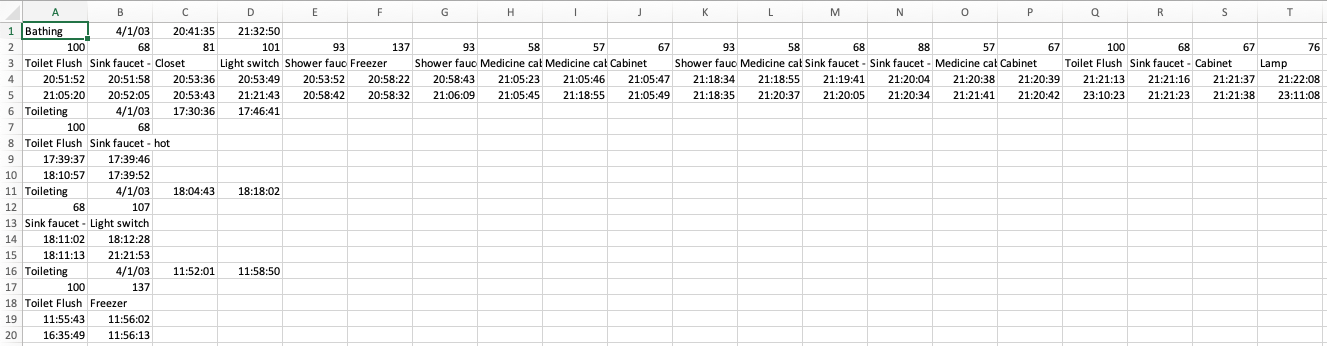
\includegraphics[width=1\linewidth]{/Users/alistairgj/Documents/GitHub/IoT_ResearchProject/IoT_November/images/s1actExcel} 

}

\caption{The S1 Activities dataset shown in a spreadsheet program. The structure of the data, a mixture of tab delimited and comma delimited values with unequal row lengths, presents a variety of challenges with respect to pre-processing}\label{fig:s1actExcel}
\end{figure}

\rowcolors{2}{gray!6}{white}
\begin{table}[!h]

\caption{\label{tab:TAB_rawDSS1}A sample of the S1 activities dataset after importation into the interactive development environment}
\centering
\fontsize{8}{10}\selectfont
\begin{tabular}[t]{ll}
\hiderowcolors
\toprule
  & 0\\
\midrule
\showrowcolors
5 & Toileting,4/1/2003,17:30:36,17:46:41\\
6 & 100,68\\
7 & Toilet Flush,Sink faucet - hot\\
8 & 17:39:37,17:39:46\\
9 & 18:10:57,17:39:52\\
\bottomrule
\end{tabular}
\end{table}
\rowcolors{2}{white}{white}

Due to the varying number of comma-separated elements in each row
(Figure \ref{fig:s1actExcel}) the \texttt{S1activities.csv} data was
imported as an indexed dataframe, containing only one column, with 1475
rows. In each row, values were comma-separated. After initial imporation
the dataframe was converted to a 2D array, using \texttt{np.array()},
where each row from the dataframe became an array within the 2D array.
The 2D array was flattened to a 1D array using \texttt{.flatten()} and
each group of observations was then chunked into a list of 5. Using the
logic shown in Algorithm \ref{alg:actExtraction}, below, the activity,
date and time data was extracted. During extraction in intermediate
activities dataset was generated as seen below in Table
\ref{tab:TAB_dsActIntermediate} followed by the tidy pre-processed
activities dataset, as seen in Table \ref{tab:TAB_dsActFinal}.

\begin{algorithm}[H]
\DontPrintSemicolon
\SetAlgoLined
\KwResult{Intermediate dataframe with 'activity', 'date', 'startTime', 'endTime' as attributes}
\SetKwInOut{Input}{Input}\SetKwInOut{Output}{Output}
\Input{S1 Activities}
\Output{S1 Activities Intermediate}
\BlankLine
\Begin{
  array1-8 = [ ]\;
  i = 0\;
  \While{i < length(dataframe)}{
    array1.append(dataframe[i][0])\;
    array2.append([x.strip() for x in array1[i].split(',')])\;
    array3.append(array2[i][0])\;
    array4.append(array2[i][1])\;
    array5.append(array2[i][2])\;
    array6.append(array2[i][3])\;
    i = i + 1\;
    }
  dfIntermediate = pandas.DataFrame(list(zip(array3, array4, array5, array6)))\;
  start = (dfIntermediate.date + " " + dfIntermediate.startTime)\;
  end = (dfIntermediate.date + " " + dfIntermediate.endTime)\;
  i = 0\;
  \While{i < length(start)}{
    array7.append(datetime.strptime(start[i], mm/dd/yyyy HH:MM:SS))\;
    array8.append(datetime.strptime(end[i], mm/dd/yyyy HH:MM:SS))\;
    i = i + 1\;
    }
  dfFinal = pandas.DataFrame(list(zip(array3, array7, array8)))\;
  \KwRet dfIntermediate\;
  \KwRet dfFinal\;
}
\caption{Extraction of data from S1 Activities dataset}
\label{alg:actExtraction}
\end{algorithm}

\pagebreak

\rowcolors{2}{gray!6}{white}
\begin{table}[!h]

\caption{\label{tab:TAB_dsActIntermediate}The S1 Activities intermediate dataset}
\centering
\fontsize{8}{10}\selectfont
\begin{tabular}[t]{llll}
\hiderowcolors
\toprule
activity & date & startTime & endTime\\
\midrule
\showrowcolors
Bathing & 4/1/2003 & 20:41:35 & 21:32:50\\
Toileting & 4/1/2003 & 17:30:36 & 17:46:41\\
Toileting & 4/1/2003 & 18:4:43 & 18:18:2\\
Toileting & 4/1/2003 & 11:52:1 & 11:58:50\\
\bottomrule
\end{tabular}
\end{table}
\rowcolors{2}{white}{white}

\rowcolors{2}{gray!6}{white}
\begin{table}[!h]

\caption{\label{tab:TAB_dsActFinal}The S1 activities tidy dataset}
\centering
\fontsize{8}{10}\selectfont
\begin{tabular}[t]{lll}
\hiderowcolors
\toprule
activity & start & end\\
\midrule
\showrowcolors
Bathing & 2003-04-01 20:41:35 & 2003-04-01 21:32:50\\
Toileting & 2003-04-01 17:30:36 & 2003-04-01 17:46:41\\
Toileting & 2003-04-01 18:04:43 & 2003-04-01 18:18:02\\
Toileting & 2003-04-01 11:52:01 & 2003-04-01 11:58:50\\
\bottomrule
\end{tabular}
\end{table}
\rowcolors{2}{white}{white}

\hypertarget{importing-visualizing-and-preprocessing-the-subactivities-data}{%
\subsection{Importing, Visualizing and Preprocessing the SubActivities
Data}\label{importing-visualizing-and-preprocessing-the-subactivities-data}}

As mentioned above, the \texttt{S1Activities\_data.csv} dataset contains
the collated activity and subactivity data from the work of Rockinson
{[}\protect\hyperlink{ref-rockinsonActivityRecognitionHome}{23}{]}. As
with the activities data extraction, the dataframe was converted to a 2D
array, using \texttt{np.array()}, where each row from the dataframe
became an array within the 2D array. The 2D array was flattened to a 1D
array using \texttt{.flatten()} and each group of observations was then
chunked into a list of 5. The sub-activity, date and time data was then
extracted from the dataset, by employing the logic shown in Algorithm
\ref{alg:subActExtraction}, below.An intermediate sub-activities dataset
was generated as seen below in Table \ref{tab:TAB_dsSUBIntermediate}
followed by the tidy pre-processed sub-activities dataset, as seen in
Table \ref{tab:TAB_dsSUBActFinal}. This dataset was exported as
\texttt{S1SubActivities\_ds.csv}.

\begin{algorithm}[H]
\DontPrintSemicolon
\SetAlgoLined
\KwResult{Intermediate dataframe with 'activity', 'date', 'startTime', 'endTime' as attributes}
\SetKwInOut{Input}{Input}\SetKwInOut{Output}{Output}
\Input{S1 Activities}
\Output{S1 Activities Intermediate}
\BlankLine
\Begin{
  array1-21 = [ ]\;
  
  \While{i < length(dataframe)}{
    array1.append(dataframe[i][0])\;
    array2.append([x.strip() for x in array1[i].split(',')])\;
    array3.append(array2[i][0])\;
    array4.append(array2[i][1])\;
    array5.append(array2[i][2])\;
    array6.append(array2[i][3])\;
    i = i + 1\;
    }
  \While{i < length(dataframe)}{
    array7.append(dataframe[i][1])\;
    array8.append([x.strip() for x in array7[i].split(',')])\;
    array9.append(dataframe[i][2])\;
    array10.append([x.strip() for x in array9[i].split(',')])\;
    array11.append(dataframe[i][3])\;
    array12.append([x.strip() for x in array11[i].split(',')])\;
    array13.append(dataframe[i][4])\;
    array14.append([x.strip() for x in array13[i].split(',')])\;
    i = i + 1\;  
    }
  \While{i < length(dataframe)}{
    for x in range(len(array8[i])) : array15.append(array4[i])\;
    i = i + 1\;  
    }
  for sublist in array8: for item in sublist: array16.append(item)\;
  for sublist in array10: for item in sublist: array17.append(item)\;
  for sublist in array12: for item in sublist: array18.append(item)\;
  for sublist in array13: for item in sublist: array19.append(item)\;
  dfIntermediate = pandas.DataFrame(list(zip(array16, array17, array15, array18, array19)))\;
  start = (dfIntermediate.date + " " + dfIntermediate.startTime)\;
  end = (dfIntermediate.date + " " + dfIntermediate.endTime)\;
  \While{i < length(start)}{
    array20.append(datetime.strptime(start[i], mm/dd/yyyy HH:MM:SS))\;
    array21.append(datetime.strptime(end[i], mm/dd/yyyy HH:MM:SS))\;
    i = i + 1\;
    }
  dfFinal = pandas.DataFrame(list(zip(array16, array17, array20, array21)))\;
  \KwRet dfIntermediate\;
  \KwRet dfFinal\;
}
\caption{Extraction of sub-activity data from S1 activities dataset}
\label{alg:subActExtraction}
\end{algorithm}

\pagebreak

\rowcolors{2}{gray!6}{white}
\begin{table}[!h]

\caption{\label{tab:TAB_dsSUBIntermediate}The S1 sub-activities intermediate dataset}
\centering
\fontsize{8}{10}\selectfont
\begin{tabular}[t]{rllll}
\hiderowcolors
\toprule
subActNum & subAct & date & startTime & endTime\\
\midrule
\showrowcolors
100 & Toilet Flush & 4/1/2003 & 20:51:52 & 21:5:20\\
68 & Sink faucet - hot & 4/1/2003 & 20:51:58 & 20:52:5\\
81 & Closet & 4/1/2003 & 20:53:36 & 20:53:43\\
101 & Light switch & 4/1/2003 & 20:53:49 & 21:21:43\\
\bottomrule
\end{tabular}
\end{table}
\rowcolors{2}{white}{white}
\rowcolors{2}{gray!6}{white}
\begin{table}[!h]

\caption{\label{tab:TAB_dsSUBActFinal}The S1 sub-activities tidy dataset}
\centering
\fontsize{8}{10}\selectfont
\begin{tabular}[t]{rlll}
\hiderowcolors
\toprule
subActNum & subAct & start & end\\
\midrule
\showrowcolors
67 & Cabinet & 2003-03-27 06:43:40 & 2003-03-27 06:43:43\\
100 & Toilet Flush & 2003-03-27 06:44:06 & 2003-03-27 07:12:41\\
101 & Light switch & 2003-03-27 06:44:20 & 2003-03-27 07:46:34\\
57 & Medicine cabinet & 2003-03-27 06:44:35 & 2003-03-27 06:44:48\\
\bottomrule
\end{tabular}
\end{table}
\rowcolors{2}{white}{white}

\hypertarget{amalgamating-duplicate-sub-activity-instances}{%
\subsubsection{Amalgamating `duplicate' sub-activity
instances}\label{amalgamating-duplicate-sub-activity-instances}}

As mentioned in above, 10 of the sensors have duplicated values, owing
to the presence of more than one sensor for certain activities. The
sub-activity \texttt{kitchen\_refrigerator}, for example, has the
numbers {[}91, 126, 144{]} associated with it, as seen in Table
\ref{tab:TAB_fridge}, below. These values are subsequently replaced with
{[}126{]}. As is the case with all sub-activities with degenerate
numbers, the end value is chosen based on the first appearance in the S1
Sensors dataset. All duplicated values, as seen in Table
\ref{tab:TAB_numDupes} were aggregated to have the same sensor ID /
subAct number, thus giving a value of n=1 with respect to
duplication.The first occurence of each degenerate subactivity provided
the subAct number to be used for all subsequent instances. This dataset
was exported as \texttt{S1SubActivities\_preprocessed.csv}.

\rowcolors{2}{gray!6}{white}
\begin{table}[!h]

\caption{\label{tab:TAB_fridge}Example of duplicate sub-activity number removal}
\centering
\resizebox{\linewidth}{!}{\fontsize{8}{10}\selectfont
\begin{tabular}[t]{rlllrlll}
\hiderowcolors
\toprule
\multicolumn{4}{c}{Prior to duplicate removal} & \multicolumn{4}{c}{Post to duplicate removal} \\
\cmidrule(l{2pt}r{2pt}){1-4} \cmidrule(l{2pt}r{2pt}){5-8}
subActNum\_pr & subAct\_pr & start\_pr & end\_pr & subActNum\_po & subAct\_po & start\_po & end\_po\\
\midrule
\showrowcolors
91 & kitchen\_refrigerator & 27/3/03 7:41 & 27/3/03 7:41 & 126 & kitchen\_refrigerator & 27/3/03 7:41 & 27/3/03 7:41\\
91 & kitchen\_refrigerator & 27/3/03 11:38 & 27/3/03 11:38 & 126 & kitchen\_refrigerator & 27/3/03 11:38 & 27/3/03 11:38\\
126 & kitchen\_refrigerator & 29/3/03 14:42 & 29/3/03 14:42 & 126 & kitchen\_refrigerator & 29/3/03 14:42 & 29/3/03 14:42\\
144 & kitchen\_refrigerator & 29/3/03 14:42 & 29/3/03 14:42 & 126 & kitchen\_refrigerator & 29/3/03 14:42 & 29/3/03 14:42\\
126 & kitchen\_refrigerator & 29/3/03 14:43 & 29/3/03 14:43 & 126 & kitchen\_refrigerator & 29/3/03 14:43 & 29/3/03 14:43\\
\bottomrule
\end{tabular}}
\end{table}
\rowcolors{2}{white}{white}

\hypertarget{addition-of-temporal-features-to-the-pre-processed-sub-activities-data}{%
\subsubsection{Addition of Temporal Features to the pre-processed
sub-activities
data}\label{addition-of-temporal-features-to-the-pre-processed-sub-activities-data}}

As noted by Basu et al, human behavior with respect to home appliance
interaction and activity, is typically periodic in nature
{[}\protect\hyperlink{ref-kaustavbasuApplianceUsagePrediction2012}{22}{]},
that is, certain activities occur at specific times of day or in a
particular sequence. It is helpful therefore to add categorical temporal
features to our dataset, in order to inform further analysis. Using the
Python \texttt{pandas} and \texttt{datetime} packages, the following
features were added to all instances of the pre-processed S1 sub
activities dataset; \texttt{dayNumeric}, \texttt{DAY}, \texttt{WDWE}
(where WD is weekday and WE is weekend), \texttt{HOUR} (based on 24-hour
time) and \texttt{durationSec} (the delta seconds value between
\texttt{start} and \texttt{end}). This dataset was exported as
\texttt{S1SubActivities\_preprocessedWfeatures.csv}.

\rowcolors{2}{gray!6}{white}
\begin{table}[!h]

\caption{\label{tab:TAB_ALL}A sample of n=1 of each sub-activity from the pre-processed dataset}
\centering
\resizebox{\linewidth}{!}{\fontsize{8}{10}\selectfont
\begin{tabular}[t]{llllllllr}
\hiderowcolors
\toprule
subActNum & subAct & start & end & dayNumeric & DAY & WDWE & HOUR & durationSec\\
\midrule
\showrowcolors
67 & bathroom\_cabinet & 2003-03-27 06:43:40 & 2003-03-27 06:43:43 & 3 & Thu & WD & 6 & 4\\
100 & bathroom\_toiletflush & 2003-03-27 06:44:06 & 2003-03-27 07:12:41 & 3 & Thu & WD & 6 & 1716\\
101 & bathroom\_lightswitch & 2003-03-27 06:44:20 & 2003-03-27 07:46:34 & 3 & Thu & WD & 6 & 3735\\
57 & bathroom\_medicinecabinet & 2003-03-27 06:44:35 & 2003-03-27 06:44:48 & 3 & Thu & WD & 6 & 14\\
82 & study\_drawer & 2003-03-27 06:45:45 & 2003-03-27 06:45:48 & 3 & Thu & WD & 6 & 4\\
\addlinespace
146 & bedroom\_drawer & 2003-03-27 06:46:12 & 2003-03-27 06:46:20 & 3 & Thu & WD & 6 & 9\\
132 & kitchen\_cabinet & 2003-03-27 06:51:43 & 2003-03-27 06:51:46 & 3 & Thu & WD & 6 & 4\\
143 & kitchen\_microwave & 2003-03-27 06:54:09 & 2003-03-27 13:07:43 & 3 & Thu & WD & 6 & 22415\\
141 & kitchen\_door & 2003-03-27 06:57:05 & 2003-03-27 06:57:08 & 3 & Thu & WD & 6 & 4\\
93 & bathroom\_showerfaucet & 2003-03-27 07:05:22 & 2003-03-27 07:05:24 & 3 & Thu & WD & 7 & 3\\
\addlinespace
125 & kitchen\_drawer & 2003-03-27 07:38:48 & 2003-03-27 07:38:51 & 3 & Thu & WD & 7 & 4\\
70 & kitchen\_dishwasher & 2003-03-27 07:40:32 & 2003-03-27 07:40:34 & 3 & Thu & WD & 7 & 3\\
126 & kitchen\_refrigerator & 2003-03-27 07:41:08 & 2003-03-27 07:41:16 & 3 & Thu & WD & 7 & 9\\
88 & bathroom\_sinkfaucet-cold & 2003-03-27 07:43:22 & 2003-03-27 07:43:48 & 3 & Thu & WD & 7 & 27\\
68 & bathroom\_sinkfaucet-hot & 2003-03-27 07:43:23 & 2003-03-27 07:43:48 & 3 & Thu & WD & 7 & 26\\
\addlinespace
140 & foyer\_door & 2003-03-27 07:48:49 & 2003-03-27 07:48:53 & 3 & Thu & WD & 7 & 5\\
137 & kitchen\_freezer & 2003-03-27 11:36:15 & 2003-03-27 11:36:21 & 3 & Thu & WD & 11 & 7\\
106 & kitchen\_burner & 2003-03-27 11:37:13 & 2003-03-27 11:42:24 & 3 & Thu & WD & 11 & 312\\
105 & kitchen\_lightswitch & 2003-03-27 11:38:54 & 2003-03-27 12:31:05 & 3 & Thu & WD & 11 & 3132\\
92 & study\_lightwitch & 2003-03-27 16:28:23 & 2003-03-27 18:44:14 & 3 & Thu & WD & 16 & 8152\\
\addlinespace
130 & bathroom\_door & 2003-03-27 17:43:10 & 2003-03-27 17:43:12 & 3 & Thu & WD & 17 & 3\\
104 & foyer\_lightswitch & 2003-03-27 19:36:32 & 2003-03-27 19:50:07 & 3 & Thu & WD & 19 & 816\\
131 & kitchen\_toaster & 2003-03-28 12:32:00 & 2003-03-28 15:10:16 & 4 & Fri & WD & 12 & 9497\\
96 & bathroom\_exhaustfan & 2003-03-28 17:43:17 & 2003-03-28 18:25:19 & 4 & Fri & WD & 17 & 2523\\
108 & bedroom\_lightswitch & 2003-03-28 18:24:48 & 2003-03-28 19:55:44 & 4 & Fri & WD & 18 & 5457\\
\addlinespace
129 & kitchen\_oven & 2003-03-28 19:09:26 & 2003-03-28 19:09:30 & 4 & Fri & WD & 19 & 5\\
56 & livingroom\_dvd & 2003-03-28 19:55:24 & 2003-03-28 19:55:29 & 4 & Fri & WD & 19 & 6\\
76 & livingroom\_lamp & 2003-03-29 13:30:51 & 2003-03-29 18:50:13 & 5 & Sat & WE & 13 & 19163\\
139 & bedroom\_jewelrybox & 2003-03-29 15:12:44 & 2003-03-29 15:12:45 & 5 & Sat & WE & 15 & 2\\
142 & kitchen\_washingmachine & 2003-03-29 15:44:24 & 2003-03-29 15:44:26 & 5 & Sat & WE & 15 & 3\\
\addlinespace
90 & kitchen\_laundrydryer & 2003-03-29 15:48:18 & 2003-03-29 15:48:54 & 5 & Sat & WE & 15 & 37\\
98 & kitchen\_garbagedisposal & 2003-03-29 15:54:50 & 2003-03-29 15:54:51 & 5 & Sat & WE & 15 & 2\\
107 & livingroom\_lightswitch & 2003-03-29 18:50:43 & 2003-03-29 18:51:09 & 5 & Sat & WE & 18 & 27\\
81 & foyer\_closet & 2003-04-01 06:13:26 & 2003-04-01 06:13:34 & 1 & Tue & WD & 6 & 9\\
145 & kitchen\_cereal & 2003-04-01 06:37:18 & 2003-04-01 06:37:59 & 1 & Tue & WD & 6 & 42\\
\addlinespace
60 & kitchen\_containers & 2003-04-01 06:38:14 & 2003-04-01 06:38:48 & 1 & Tue & WD & 6 & 35\\
119 & kitchen\_coffeemachine & 2003-04-09 08:46:07 & 2003-04-09 08:46:35 & 2 & Wed & WD & 8 & 29\\
64 & bedroom\_lamp & 2003-04-09 20:16:36 & 2003-04-09 21:13:19 & 2 & Wed & WD & 20 & 3404\\
\bottomrule
\end{tabular}}
\end{table}
\rowcolors{2}{white}{white}

\pagebreak

\hypertarget{subactivity-visualisation-and-outlier-inspection}{%
\subsubsection{SubActivity Visualisation and Outlier
Inspection}\label{subactivity-visualisation-and-outlier-inspection}}

\hypertarget{aggregated-line-chart}{%
\paragraph{Aggregated Line Chart}\label{aggregated-line-chart}}

The \texttt{S1SubActivities\_preprocessedWfeatures.csv} dataset was
analysed using data visualisation techniques. A plot of aggregated
sub-activity count versus sub-activity was generated, as seen in Figure
\ref{fig:FIG_aggLineChart}, below. The chart shows that there is a high
level of consistency with respect to the overall aggregated count of
each sub-activity, when compared to the feature
\texttt{Day\ of\ the\ Week}.

\begin{figure}[H]

{\centering 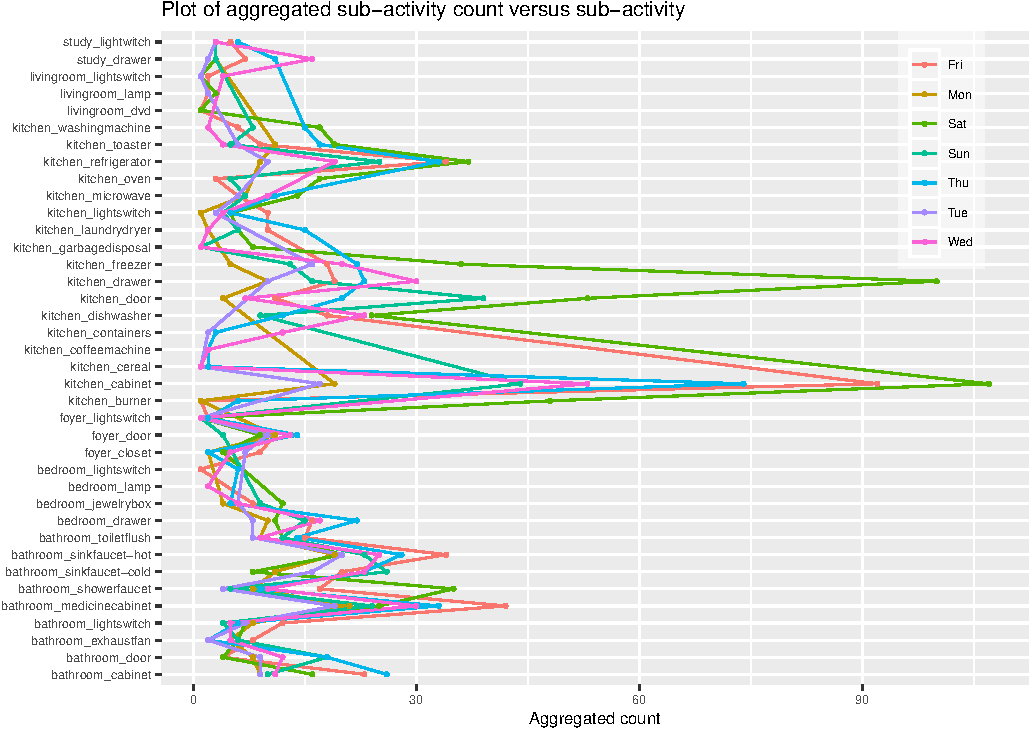
\includegraphics{MD_Final_files/figure-latex/FIG_aggLineChart-1} 

}

\caption{Aggregated line chart}\label{fig:FIG_aggLineChart}
\end{figure}

\pagebreak

\hypertarget{aggregated-box-plot-of-sub-activities}{%
\paragraph{Aggregated Box Plot of
Sub-Activities}\label{aggregated-box-plot-of-sub-activities}}

Figure \ref{fig:FIG_allBoxPlots}, below, shows boxplots of all
sub-activities versus their duration values. In this plot, we can see
many outliers, which will inform further analysis. We also note that
many of the outliers are extremely unrealistic. Of particular concern
Kitchen\_Toaster with a duration of almost 30,000 seconds,
Bathroom\_toiletflush distributed up to the range of 20,000 seconds.
This potentially indicates challenges with the initial data collection
methodology or experimental conditions / setup. Each sub-activity will
be individually considered with respect to it's outliers.

\begin{figure}[H]

{\centering 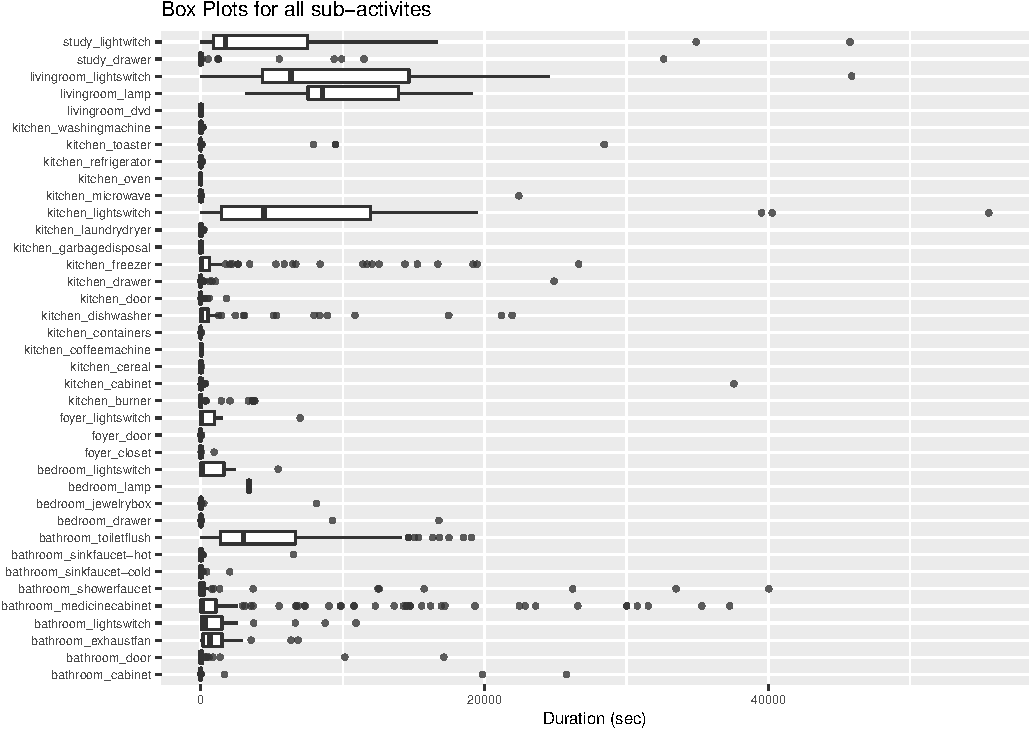
\includegraphics{MD_Final_files/figure-latex/FIG_allBoxPlots-1} 

}

\caption{Box plots for all sub-activites}\label{fig:FIG_allBoxPlots}
\end{figure}

\hypertarget{sub-activity-data-cleansing}{%
\subsubsection{Sub-Activity Data
Cleansing}\label{sub-activity-data-cleansing}}

Via the inspection of each sub-activity the following set of instances
were identified, as seen in Table \ref{tab:outlierSTATS}. In all cases
the standard deviation of each aggregated instance (n=Count) is found to
be greater than the mean, indicating that the data points are not even
distributed with respect to total duration of the sub-activity,
additionally, the median in all cases is found to be vastly different
from the mean. The bathroom medicine cabinet, for example, has a mean
value of 3188 seconds (53 minutes) and a median value of 88 seconds.
Accross all sub-activities seen in Table \ref{tab:outlierSTATS}, the
median gives more reasonable values. Therefore the median value for each
sub-activity below will be used to fill the outlier values. There were
in total 4 pre-processing methodologies used. 1. Filling outliers with
median 2. All values replaced with one value 3. No further processing
required 4. Sub-activity dropped

\rowcolors{2}{gray!6}{white}
\begin{table}[!h]

\caption{\label{tab:outlierSTATS}Summary table of outliers with respect to sub-activity duration over all instances}
\centering
\fontsize{8}{10}\selectfont
\begin{tabular}[t]{lrrrr}
\hiderowcolors
\toprule
SubAct & Count & Median & Mean & Std\\
\midrule
\showrowcolors
bathroom\_cabinet & 104 & 4.0 & 460.22115 & 3176.1633\\
bathroom\_medicinecabinet & 194 & 88.0 & 3188.97423 & 7354.1424\\
study\_drawer & 45 & 6.0 & 1634.48889 & 5432.4063\\
bedroom\_drawer & 99 & 10.0 & 273.47475 & 1918.7262\\
kitchen\_cabinet & 406 & 7.0 & 112.82020 & 1864.0122\\
\addlinespace
kitchen\_microwave & 61 & 6.0 & 377.40984 & 2868.6679\\
kitchen\_door & 134 & 4.0 & 46.11194 & 174.1857\\
bathroom\_showerfaucet & 88 & 15.0 & 1754.35227 & 6540.7295\\
kitchen\_drawer & 208 & 4.0 & 145.06250 & 1727.5767\\
bathroom\_sinkfaucet-hot & 169 & 11.0 & 57.90533 & 501.2729\\
\addlinespace
kitchen\_freezer & 130 & 39.0 & 1738.10769 & 4512.5738\\
bathroom\_door & 73 & 17.0 & 461.61644 & 2310.8116\\
kitchen\_toaster & 71 & 5.0 & 790.36620 & 3793.6744\\
kitchen\_lightswitch & 32 & 4454.0 & 9318.71875 & 13081.3404\\
study\_lightwitch & 26 & 1728.5 & 6430.73077 & 11002.3025\\
\addlinespace
kitchen\_dishwasher & 86 & 63.5 & 1518.40698 & 4146.6375\\
livingroom\_lightswitch & 8 & 6352.5 & 12545.12500 & 15556.6628\\
foyer\_closet & 29 & 8.0 & 42.44828 & 174.4286\\
\bottomrule
\end{tabular}
\end{table}
\rowcolors{2}{white}{white}

\hypertarget{sub-activity-cleansing---1-filling-outliers-with-median}{%
\subsubsection{Sub-Activity Cleansing - 1) Filling outliers with
median}\label{sub-activity-cleansing---1-filling-outliers-with-median}}

This methodology was also applied to all of the other sub-activities in
Table \ref{tab:outlierSTATS}.

\hypertarget{bathroom-cabinet---sub-activity-67}{%
\paragraph{Bathroom Cabinet - Sub-Activity
67}\label{bathroom-cabinet---sub-activity-67}}

As per Table \ref{tab:outlierSTATS}, above, the bathroom cabinet has an
overall count of n=104 in the dataset. In Figure \ref{fig:subAct67} the
boxplot (A) in row one shows several outliers, most notably around the
20,000 second mark for Friday and the 25,000 mark for Sunday. When
considering all weekday and weekend values together, the mean is found
to be 460.22 seconds, while the standard deviation is found to be
3176.16. As the SD in this case greatly overwhelms the mean, and the
values of 20,000 seconds and 25,000 seconds are highly unrealistic for
the sub-activity in question, the outliers will be filled with the
median (4.0 seconds). The resultant plots can be seen in the second row.

\begin{figure}[H]

{\centering 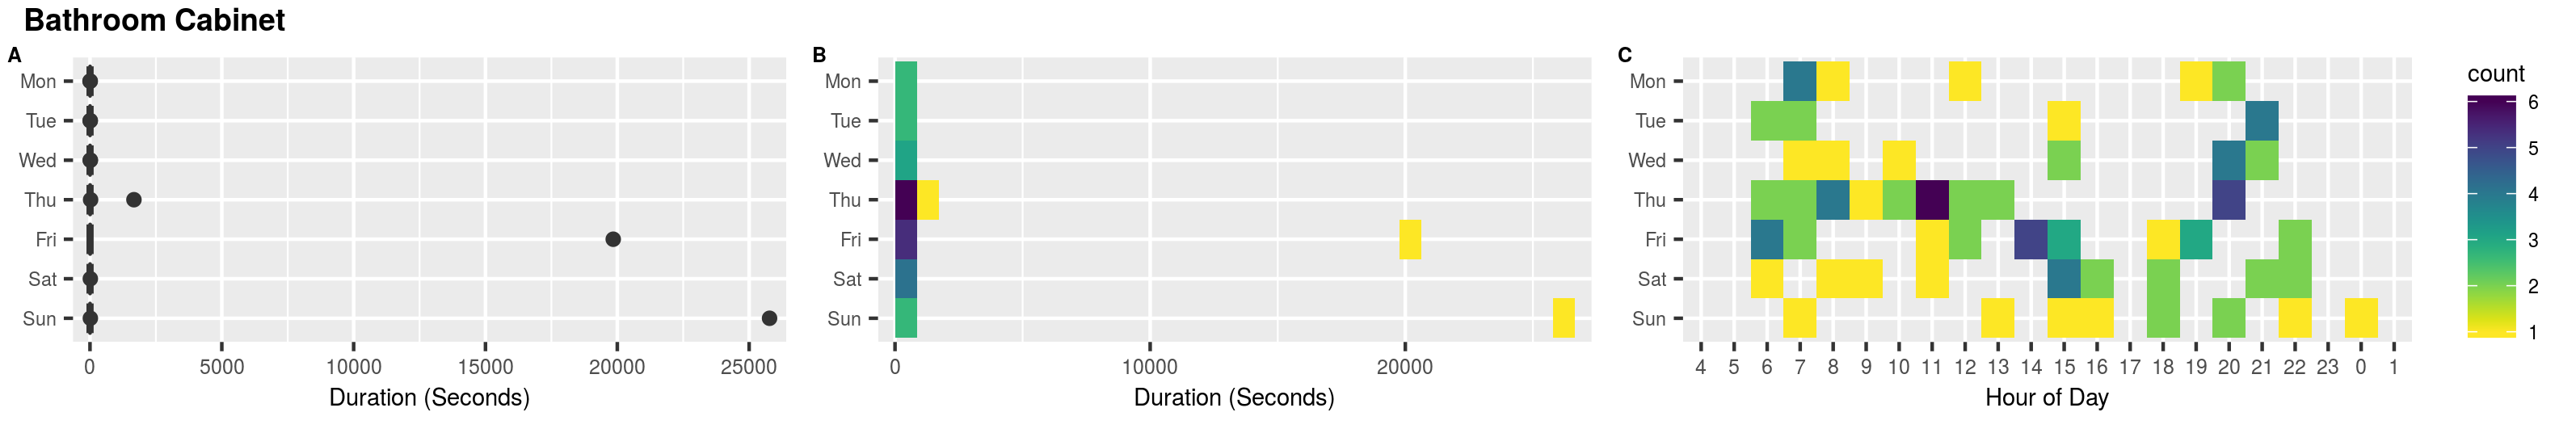
\includegraphics[width=1\linewidth]{/Users/alistairgj/Documents/GitHub/IoT_ResearchProject/IoT_November/images/subAct67} 

}

\caption{Initial and processed data box plot (A) and heat maps (B = day of week versus duration in seconds mapped by count, C = day of week versus hour of day mapped by count) for the bathroom cabinet sub-activity.}\label{fig:subAct67}
\end{figure}

\hypertarget{bathroom-medicine-cabinet---sub-activity-57}{%
\paragraph{Bathroom Medicine Cabinet - Sub-Activity
57}\label{bathroom-medicine-cabinet---sub-activity-57}}

The bathroom medicine cabinet has an overall count of n=194 in the
dataset. In Figure \ref{fig:subAct57} boxplot (A) in row one shows a
large amount of outliers, ranging all the way to nearly 40,000 seconds
(over 11 hours). This is clearly outside the expected range for this
sub-activity, with a median of 88.0 seconds, a mean of 460.22 seconds,
and a standard deviation of 7354.14 seconds. These outliers will be
filled with the median (88.0 seconds). The resultant plots can be seen
in the second row.

\begin{figure}[H]

{\centering 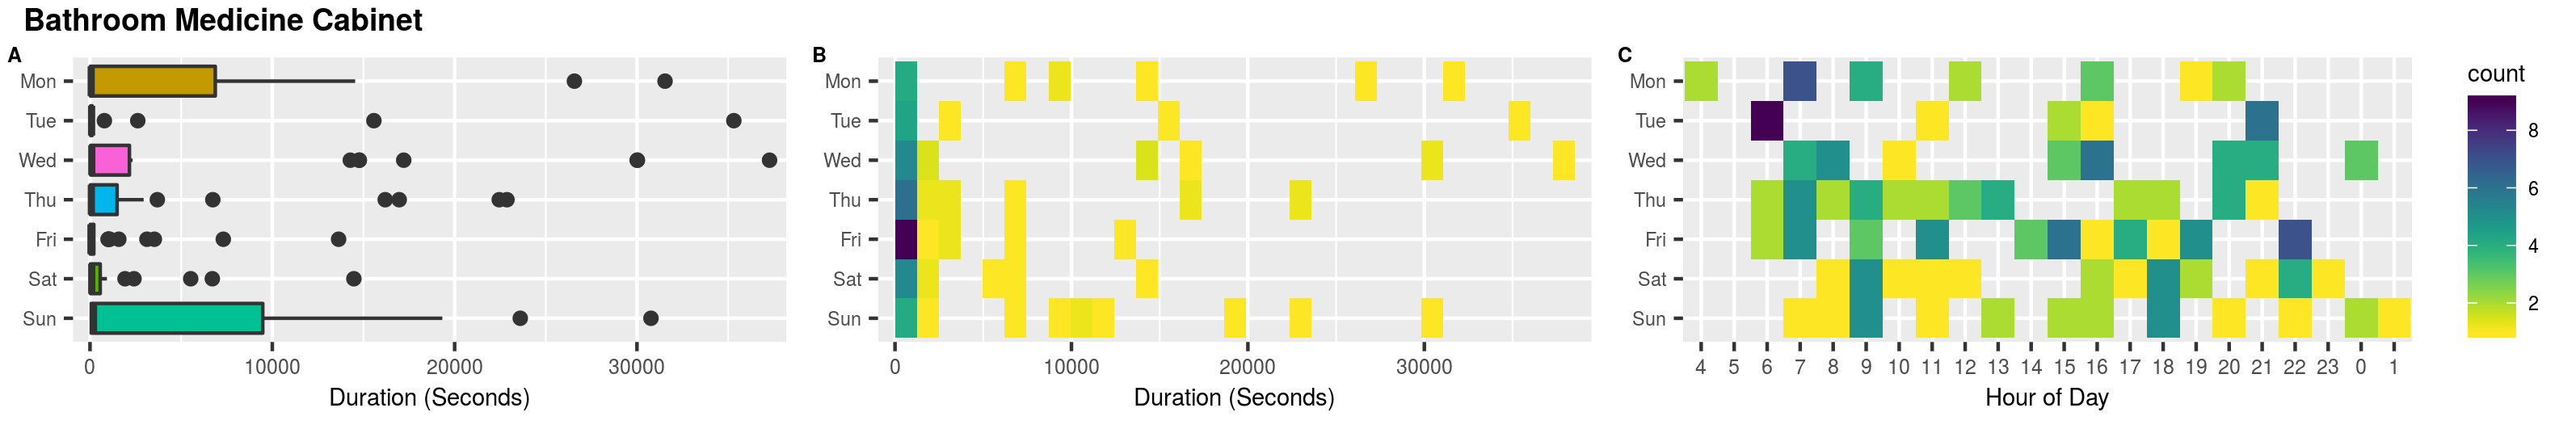
\includegraphics[width=1\linewidth]{/Users/alistairgj/Documents/GitHub/IoT_ResearchProject/IoT_November/images/subAct57} 

}

\caption{Initial and processed data box plot (A) and heat maps (B = day of week versus duration in seconds mapped by count, C = day of week versus hour of day mapped by count) for the Bathroom Medicine Cabinet sub activity.}\label{fig:subAct57}
\end{figure}

\hypertarget{study-drawer---sub-activity-82}{%
\paragraph{Study Drawer - Sub-Activity
82}\label{study-drawer---sub-activity-82}}

The study drawer has an overall count of n=45 in the dataset. In Figure
\ref{fig:subAct82} boxplot (A) in row one shows some abnormal results
for Monday, Friday and Saturday. While the median is 6.0 seconds, there
are results for Saturday that stretch beyond 30,000 seconds, clearly
indicating sensor or measurement error. It is also outside the expected
range for this sub-activity, causing the mean to be 1634.49 seconds with
a standard deviation of 5432.41 seconds. These outliers will be filled
with the median (6.0 seconds). The resultant plots can be seen in the
second row.

\begin{figure}[H]

{\centering 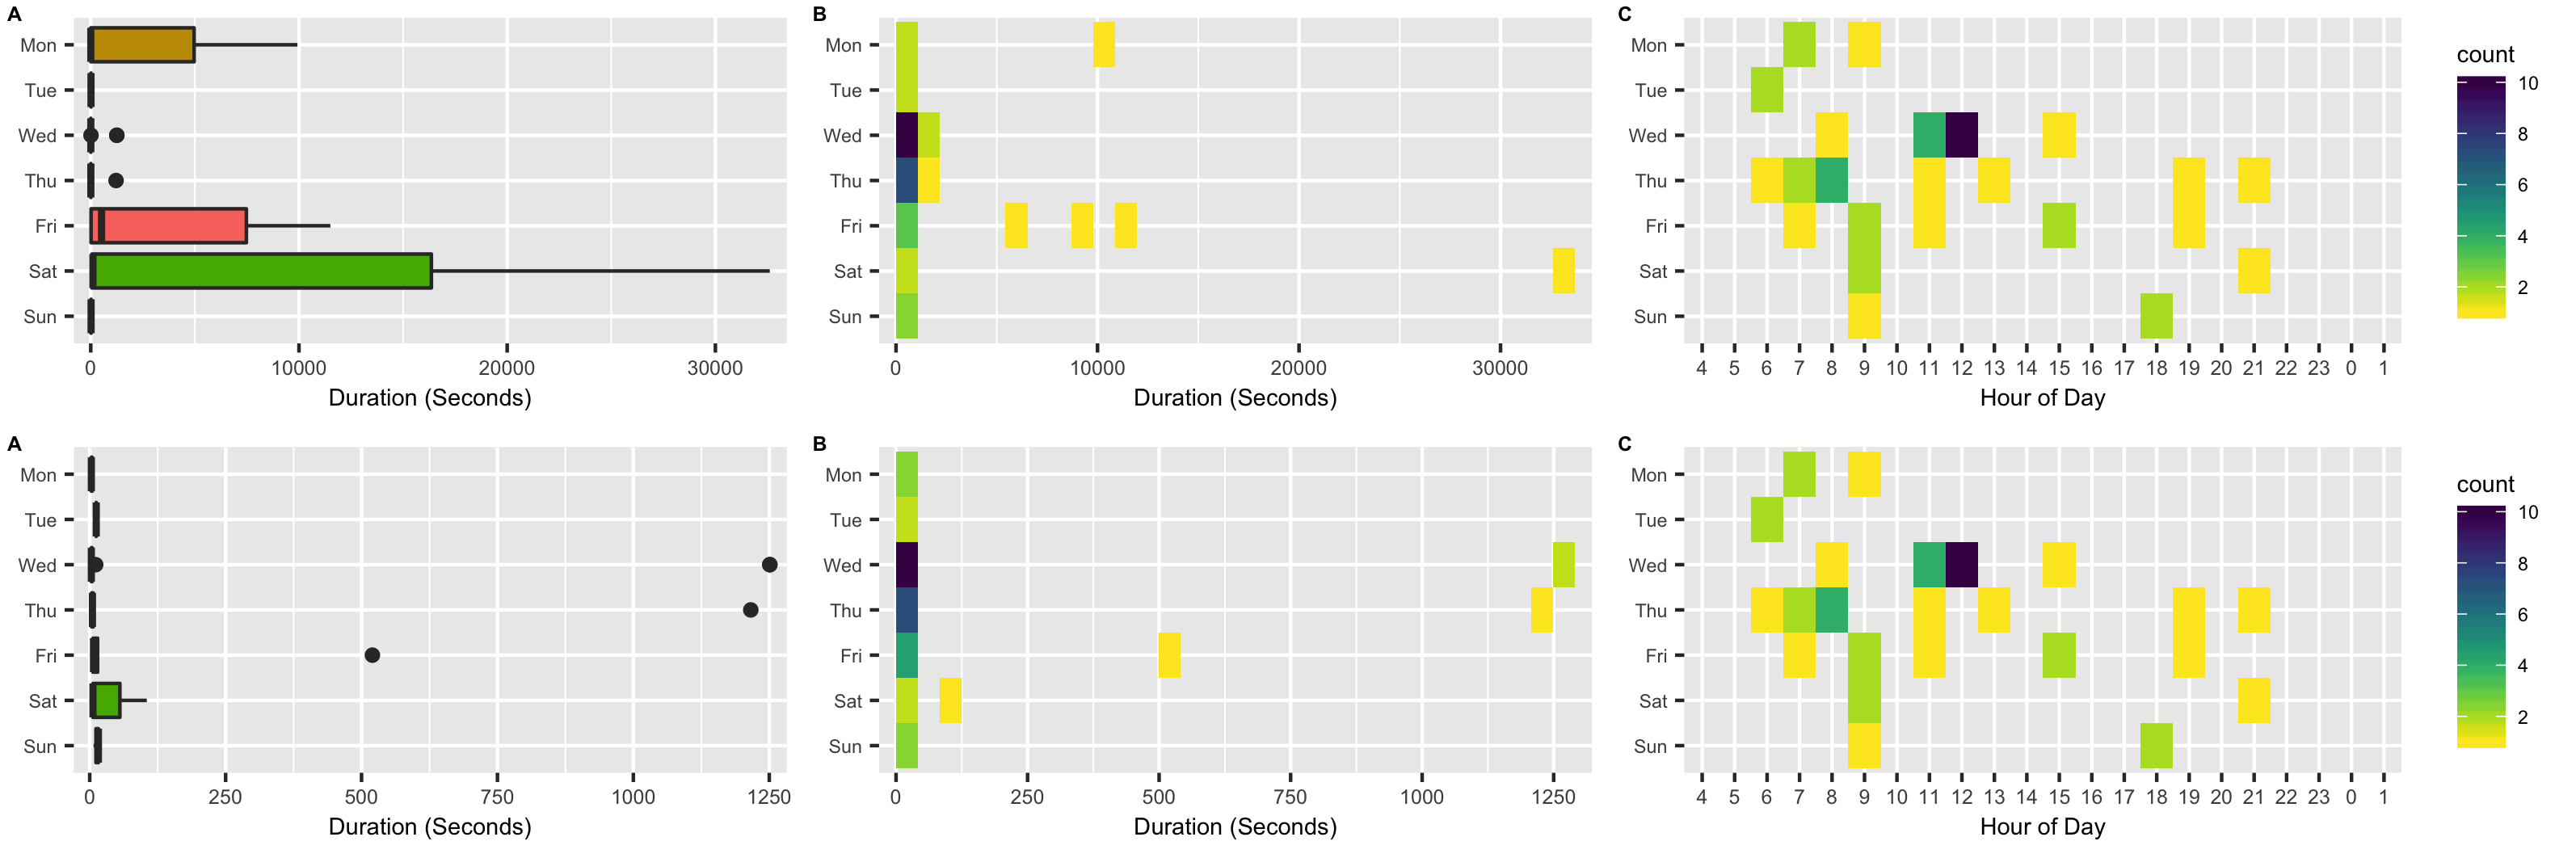
\includegraphics[width=1\linewidth]{/Users/alistairgj/Documents/GitHub/IoT_ResearchProject/IoT_November/images/subAct82} 

}

\caption{Initial and processed data box plot (A) and heat maps (B = day of week versus duration in seconds mapped by count, C = day of week versus hour of day mapped by count) for the Study Drawer sub activity.}\label{fig:subAct82}
\end{figure}

\hypertarget{bedroom-drawer---sub-activity-146}{%
\paragraph{Bedroom Drawer - Sub-Activity
146}\label{bedroom-drawer---sub-activity-146}}

The bedroom drawer has an overall count of n=99. In Figure
\ref{fig:subAct146} boxplot (A) in row one shows two main outliers, one
on Friday at just under 10,000 seconds, and one on Wednesday at around
17,000 seconds. The median for this sub-activity is 10.0 seconds, and
such outliers are clearly outside the expected range for this
sub-activity, causing the mean to be 273.47 seconds with a standard
deviation of 1918.73 seconds. These outliers will be filled with the
median (10.0 seconds). The resultant plots can be seen in the second
row.

\begin{figure}[H]

{\centering 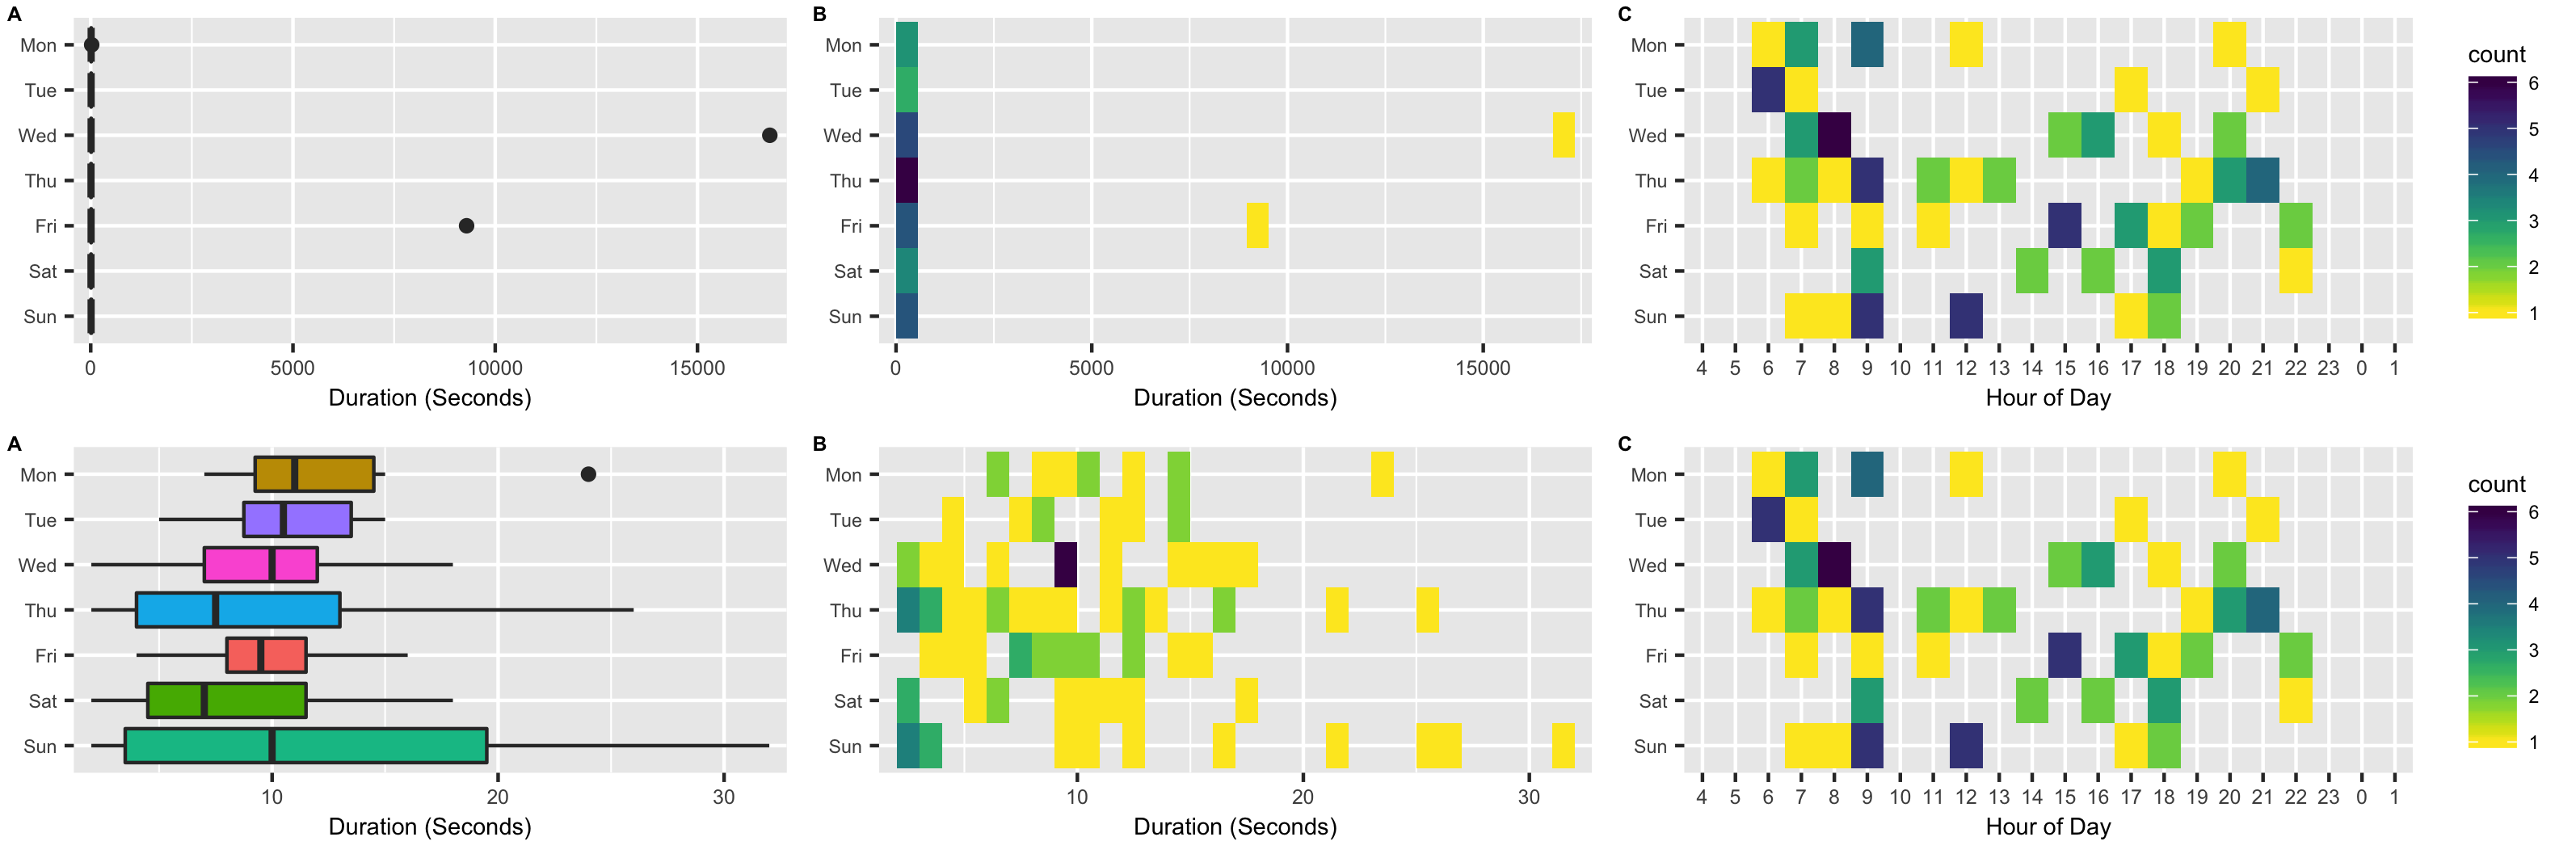
\includegraphics[width=1\linewidth]{/Users/alistairgj/Documents/GitHub/IoT_ResearchProject/IoT_November/images/subAct146} 

}

\caption{Initial and processed data box plot (A) and heat maps (B = day of week versus duration in seconds mapped by count, C = day of week versus hour of day mapped by count) for the Bedroom Drawer sub activity.}\label{fig:subAct146}
\end{figure}

\hypertarget{kitchen-cabinet---sub-activity-132}{%
\paragraph{Kitchen Cabinet - Sub-Activity
132}\label{kitchen-cabinet---sub-activity-132}}

The kitchen cabinet has an overall count of n=406. Figure
\ref{fig:subAct132} boxplot (A) in row one shows one main outlier on
Tuesday, at nearly 40,000 seconds. The median for this sub-activity is
7.0 seconds, and this outlier is clearly outside the expected range for
this sub-activity, causing the mean to be 112.82 seconds with a standard
deviation of 1864.01 seconds. This outlier will be filled with the
median (7.0 seconds). The resultant plots can be seen in the second row.

\begin{figure}[H]

{\centering 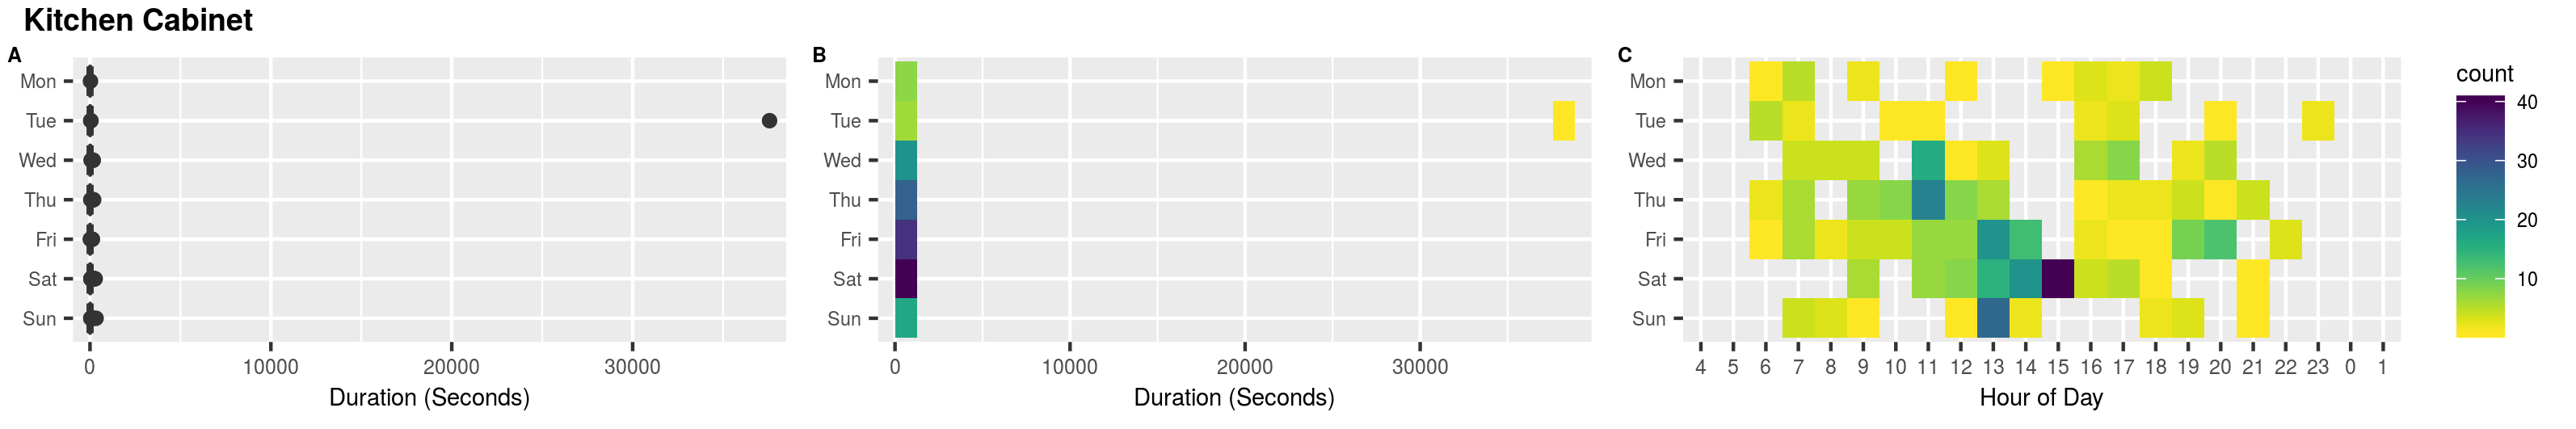
\includegraphics[width=1\linewidth]{/Users/alistairgj/Documents/GitHub/IoT_ResearchProject/IoT_November/images/subAct132} 

}

\caption{Initial and processed data box plot (A) and heat maps (B = day of week versus duration in seconds mapped by count, C = day of week versus hour of day mapped by count) for the Kitchen Cabinet sub activity.}\label{fig:subAct132}
\end{figure}

\hypertarget{kitchen-microwave---sub-activity-143}{%
\paragraph{Kitchen Microwave - Sub-Activity
143}\label{kitchen-microwave---sub-activity-143}}

The kitchen microwave has an overall count of n=61.Figure
\ref{fig:subAct143} boxplot (A) in row one shows one main outlier on
Thursday, at nearly 22,500 seconds. The median for this sub-activity is
6.0 seconds, and this outlier is clearly outside the expected range for
this sub-activity, causing the mean to be 377.41 seconds with a standard
deviation of 2868.67 seconds. This outlier will be filled with the
median (6.0 seconds). The resultant plots can be seen in the second row.

\begin{figure}[H]

{\centering 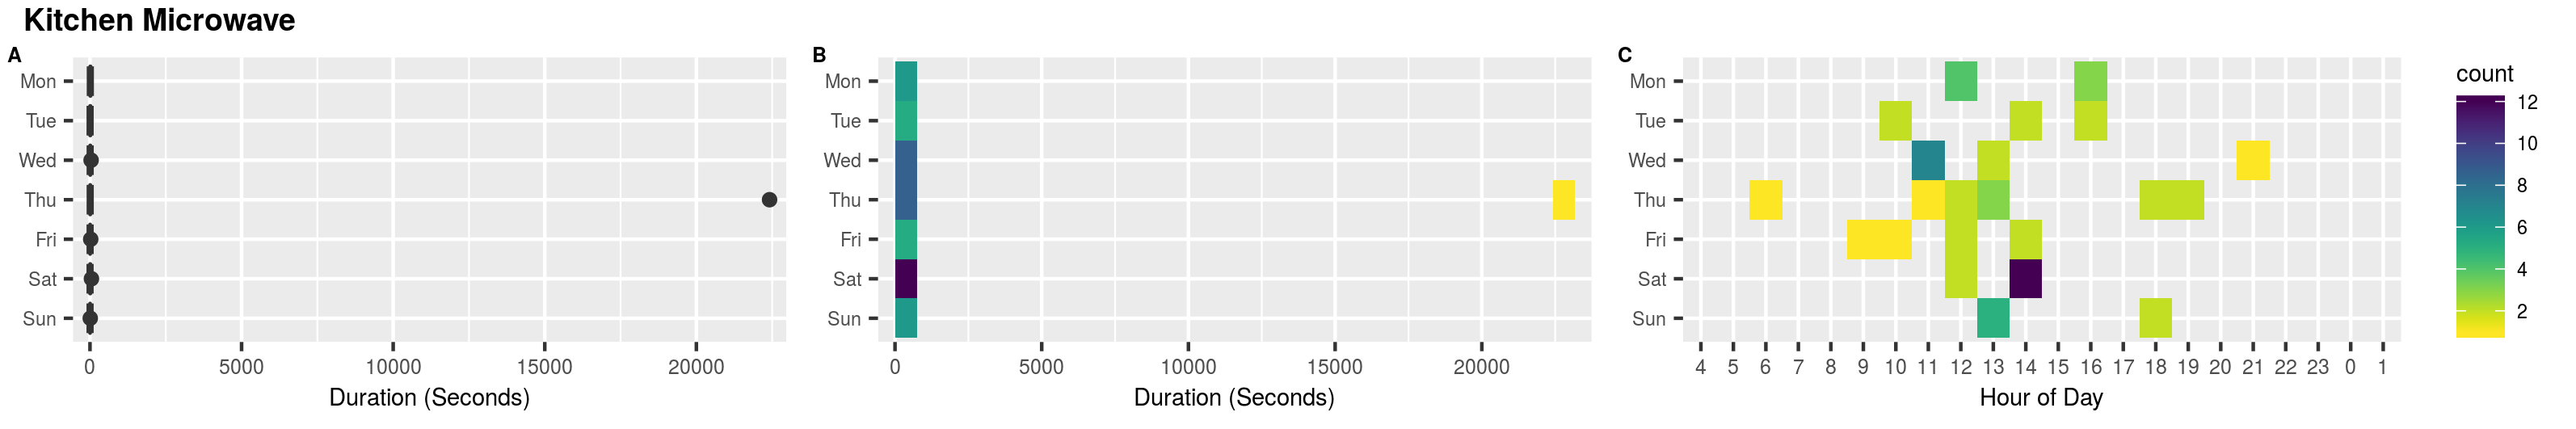
\includegraphics[width=1\linewidth]{/Users/alistairgj/Documents/GitHub/IoT_ResearchProject/IoT_November/images/subAct143} 

}

\caption{Initial and processed data box plot (A) and heat maps (B = day of week versus duration in seconds mapped by count, C = day of week versus hour of day mapped by count) for the Kitchen Microwave sub activity.}\label{fig:subAct143}
\end{figure}

\hypertarget{kitchen-door---sub-activity-141}{%
\paragraph{Kitchen Door - Sub-Activity
141}\label{kitchen-door---sub-activity-141}}

The kitchen door has an overall count of n=134. Figure
\ref{fig:subAct141} boxplot (A) in row one shows several key outliers,
notably one on Friday at over 1,750 seconds. The median for this
sub-activity is 4.0 seconds, and these outliers are clearly outside the
expected range for this sub-activity, causing the mean to be 46.11
seconds with a standard deviation of 174.19 seconds. These outliers will
be filled with the median (4.0 seconds). The resultant plots can be seen
in the second row.

\begin{figure}[H]

{\centering 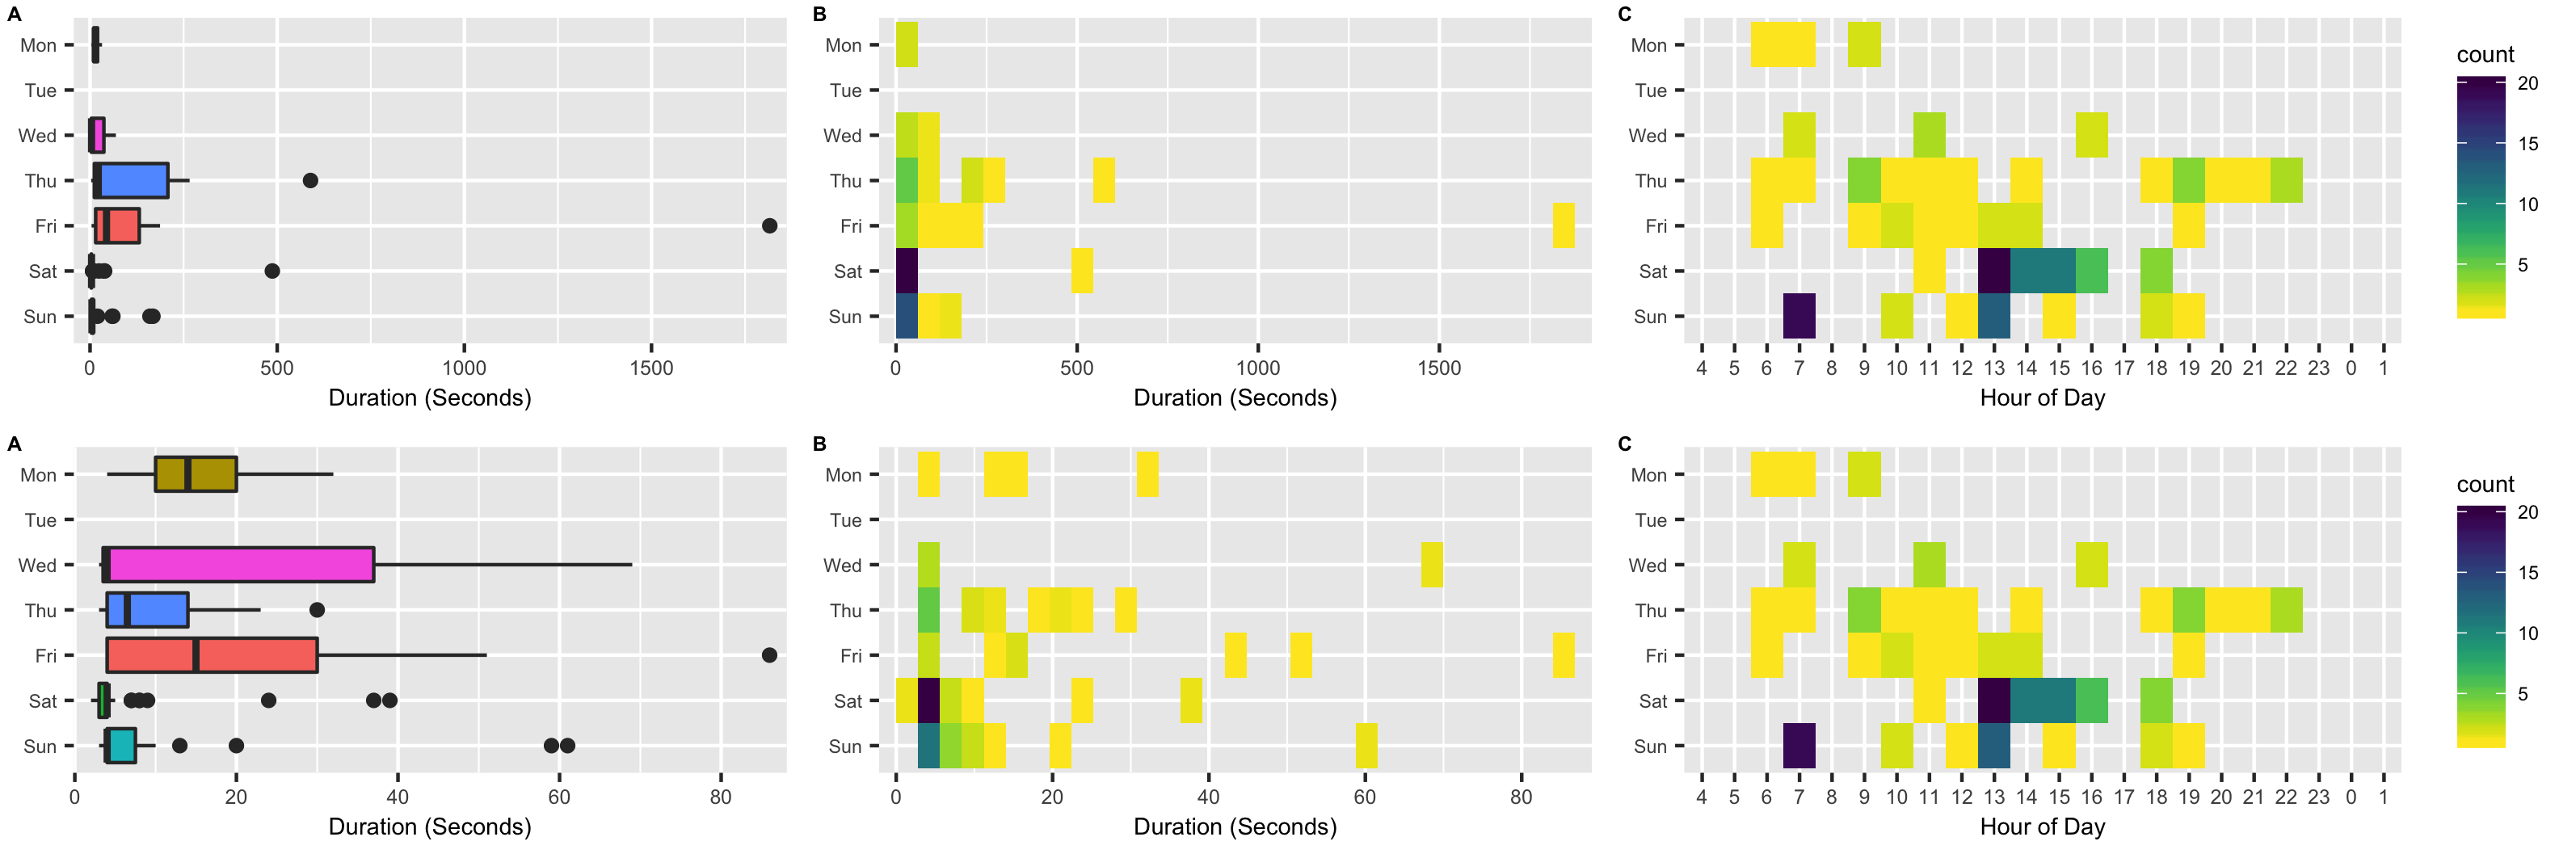
\includegraphics[width=1\linewidth]{/Users/alistairgj/Documents/GitHub/IoT_ResearchProject/IoT_November/images/subAct141} 

}

\caption{Initial and processed data box plot (A) and heat maps (B = day of week versus duration in seconds mapped by count, C = day of week versus hour of day mapped by count) for the Kitchen Door sub activity.}\label{fig:subAct141}
\end{figure}

\hypertarget{bathroom-shower-faucet---sub-activity-93}{%
\paragraph{Bathroom Shower Faucet - Sub-Activity
93}\label{bathroom-shower-faucet---sub-activity-93}}

The bathroom shower faucet has an overall count of n=88. Figure
\ref{fig:subAct93} boxplot (A) in row one shows several outliers, with
six of particular concern that range from over 10,000 seconds to 40,000
seconds. The median for this sub-activity is 15.0 seconds, and these
extreme outliers are clearly outside the expected range for this
sub-activity, causing the mean to be 1754.35 seconds with a standard
deviation of 6540.73 seconds. The outliers will be filled with the
median (15.0 seconds). The resultant plots can be seen in the second
row.

\begin{figure}[H]

{\centering 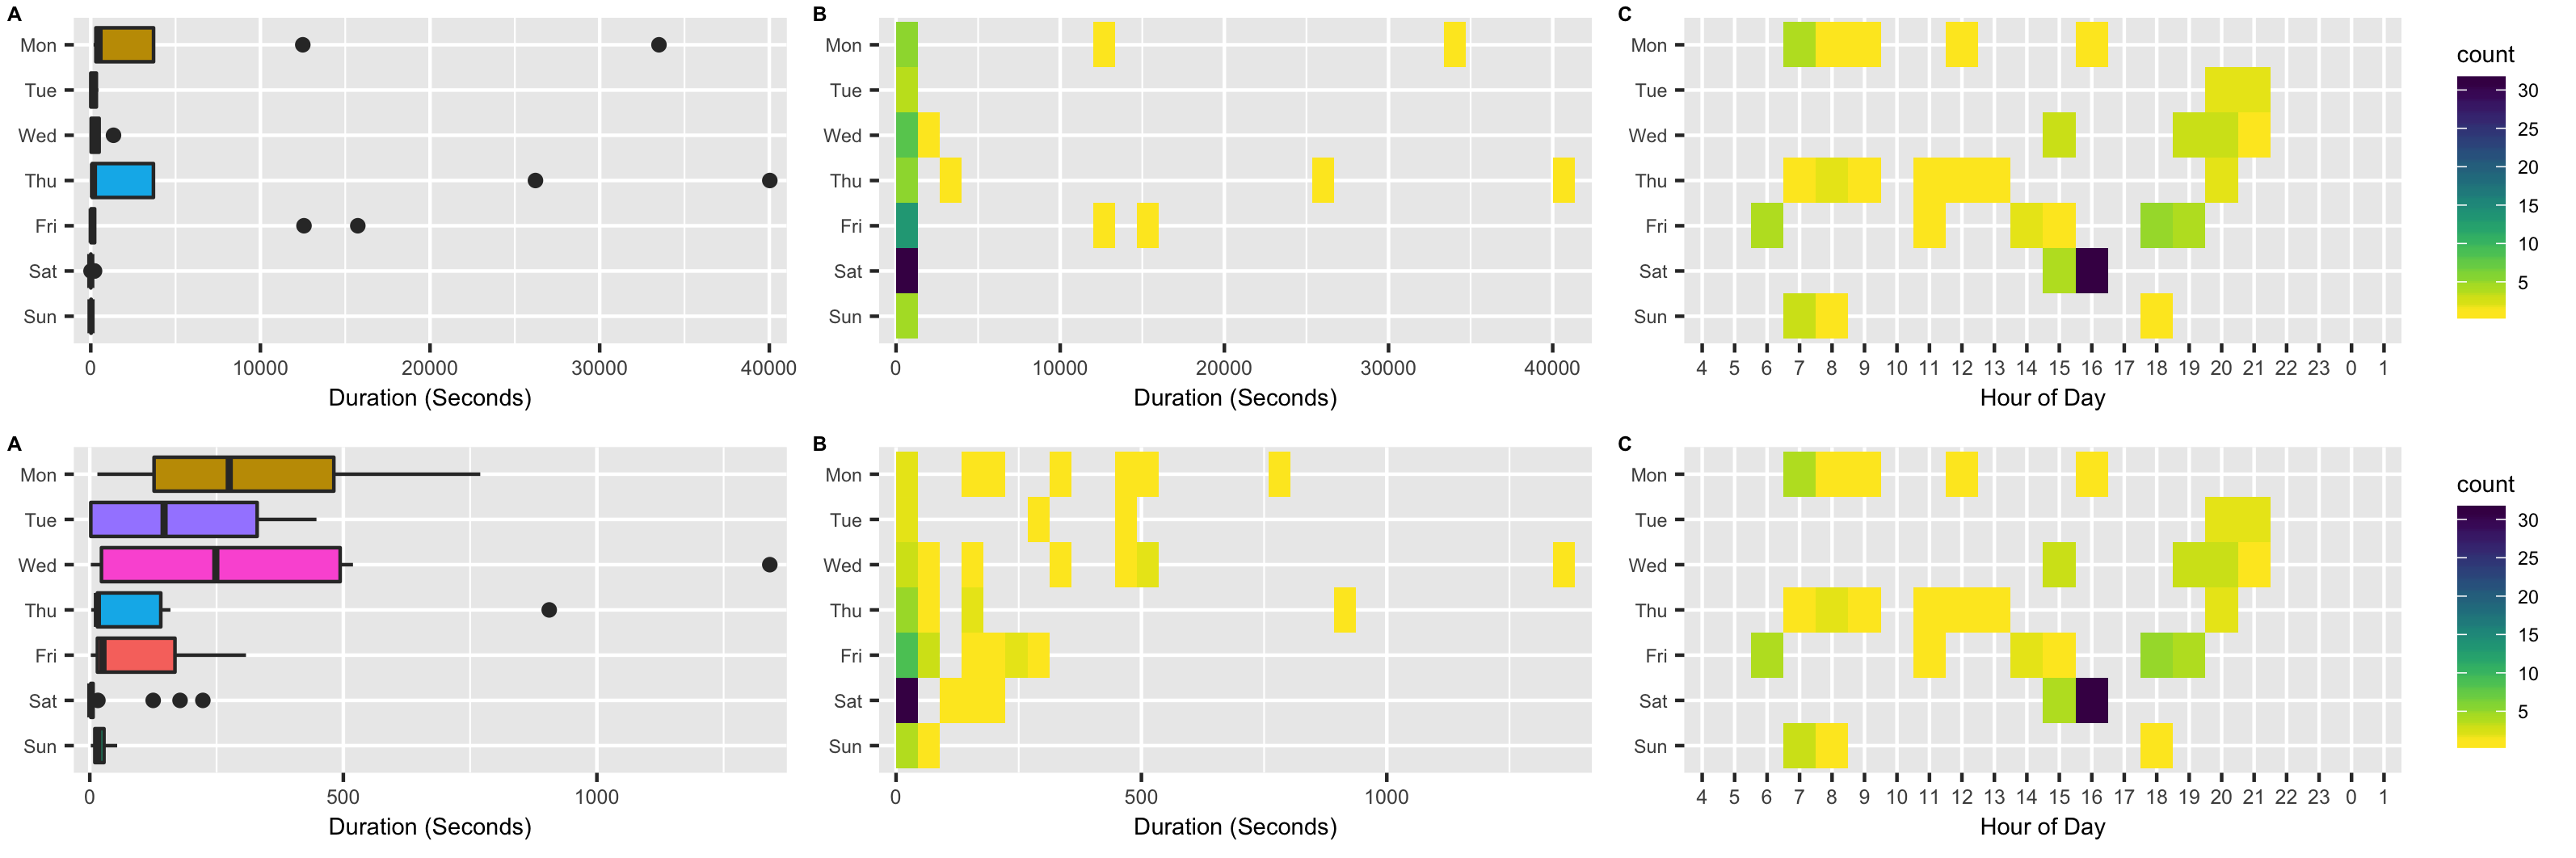
\includegraphics[width=1\linewidth]{/Users/alistairgj/Documents/GitHub/IoT_ResearchProject/IoT_November/images/subAct93} 

}

\caption{Initial and processed data box plot (A) and heat maps (B = day of week versus duration in seconds mapped by count, C = day of week versus hour of day mapped by count) for the Bathroom Shower Faucet sub activity.}\label{fig:subAct93}
\end{figure}

\hypertarget{kitchen-drawer---sub-activity-125}{%
\paragraph{Kitchen Drawer - Sub-Activity
125}\label{kitchen-drawer---sub-activity-125}}

The kitchen drawer has an overall count of n=208. Figure
\ref{fig:subAct125} boxplot (A) in row one shows one main outlier on
Sunday, at nearly 25,000 seconds. The median for this sub-activity is
4.0 seconds, and this outlier is clearly outside the expected range for
this sub-activity, causing the mean to be 145.06 seconds with a standard
deviation of 1727.58 seconds. This outlier will be filled with the
median (4.0 seconds). The resultant plots can be seen in the second row.

\begin{figure}[H]

{\centering 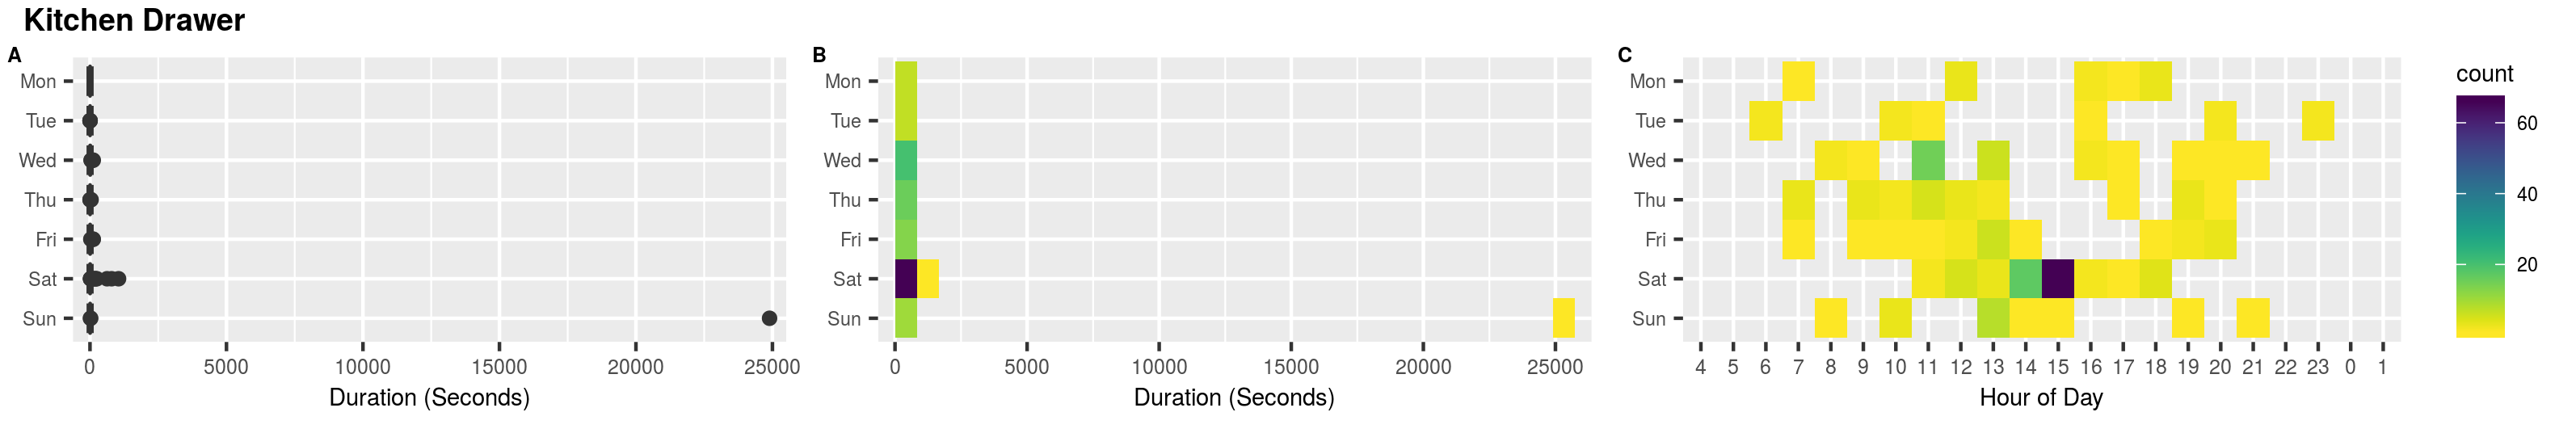
\includegraphics[width=1\linewidth]{/Users/alistairgj/Documents/GitHub/IoT_ResearchProject/IoT_November/images/subAct125} 

}

\caption{Initial and processed data box plot (A) and heat maps (B = day of week versus duration in seconds mapped by count, C = day of week versus hour of day mapped by count) for the Kitchen Drawer sub activity.}\label{fig:subAct125}
\end{figure}

\hypertarget{kitchen-dishwasher---sub-activity-70}{%
\paragraph{Kitchen Dishwasher - Sub-Activity
70}\label{kitchen-dishwasher---sub-activity-70}}

The kitchen dishwasher has an overall count of n=86. Figure
\ref{fig:subAct70} boxplot (A) in row one shows several outliers,
particularly six in the range of 7500 seconds to nearly 25,000 seconds.
The observations for Thursdays are also much higher on average than the
observations for the other days. The median for this sub-activity is
63.5 seconds, and these outliers and abnormal results are clearly
outside the expected range for this sub-activity, causing the mean to be
1518.41 seconds with a standard deviation of 4146.64 seconds. These
outliers will be filled with the median (63.5 seconds). The resultant
plots can be seen in the second row.

\begin{figure}[H]

{\centering 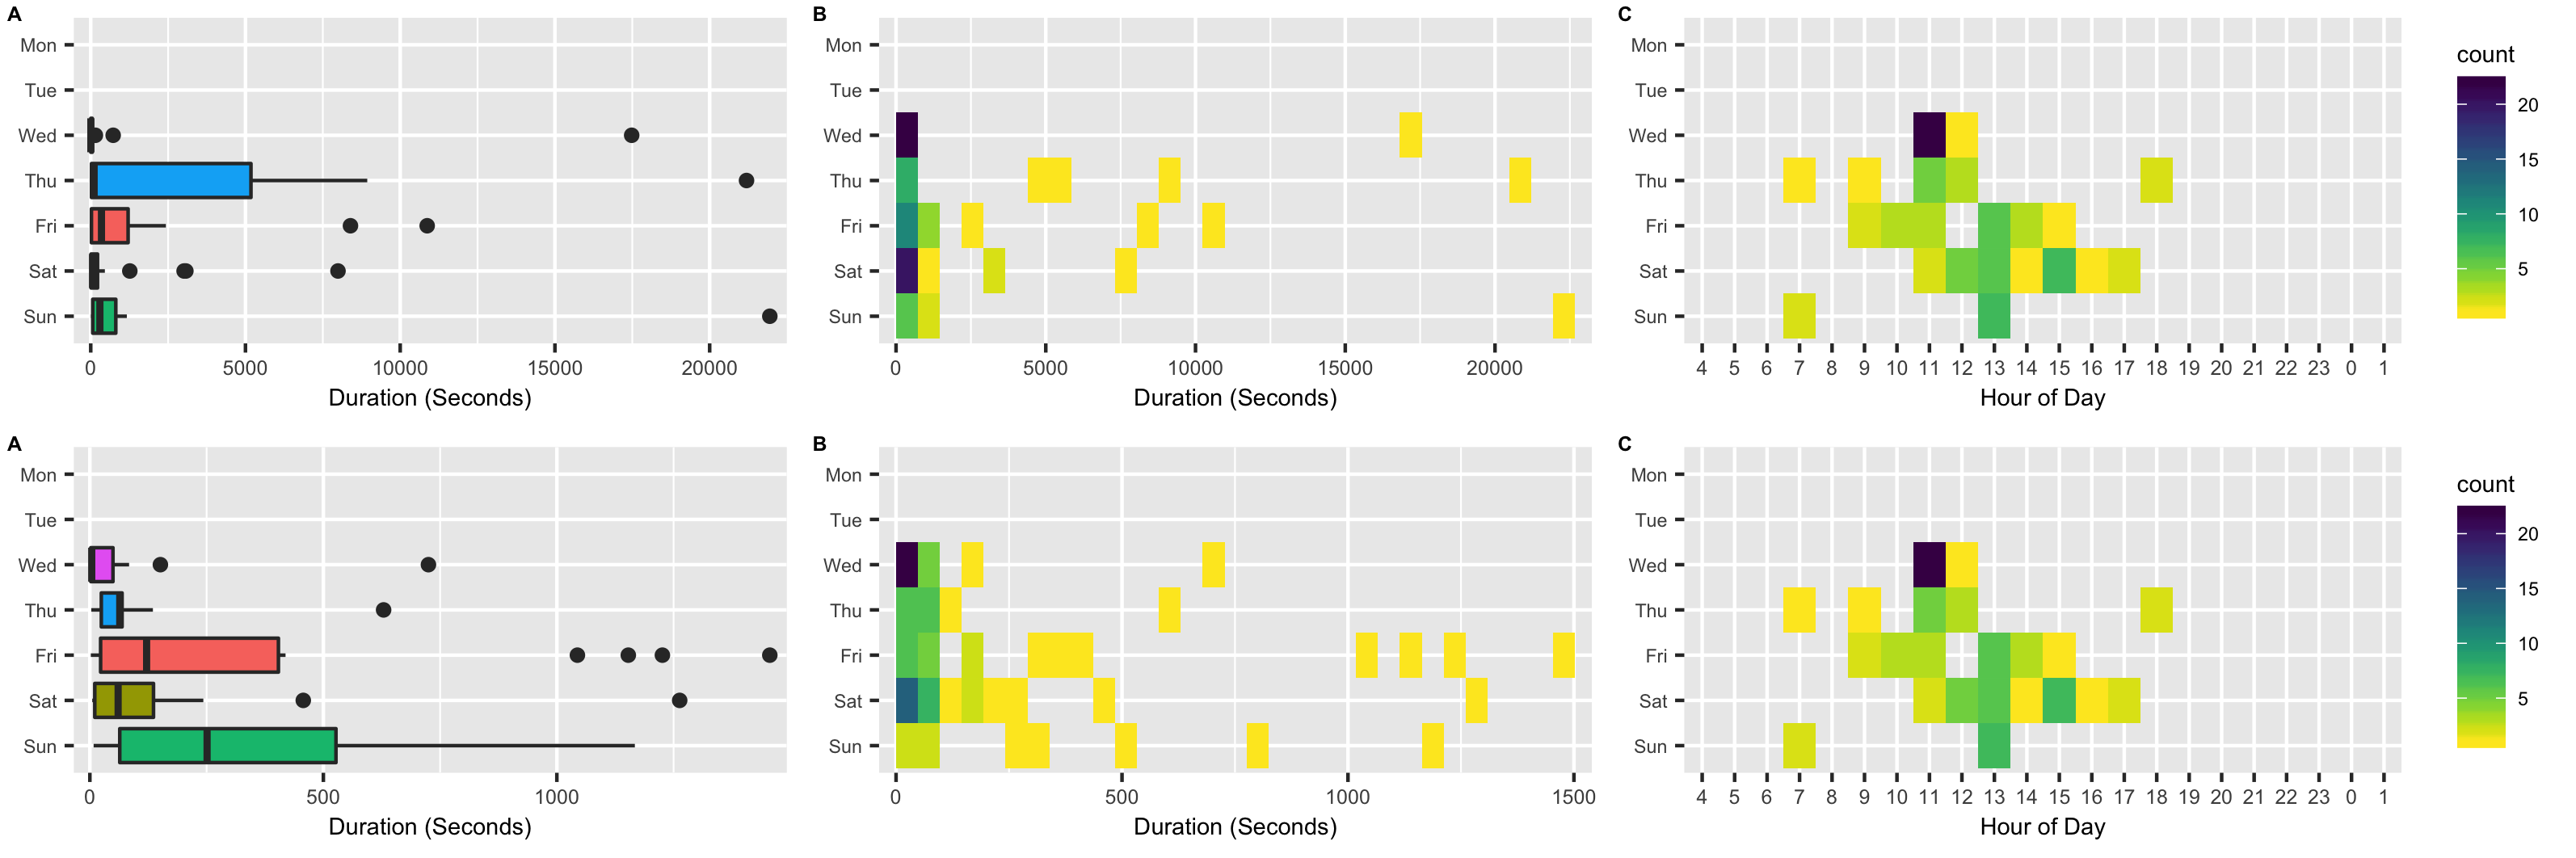
\includegraphics[width=1\linewidth]{/Users/alistairgj/Documents/GitHub/IoT_ResearchProject/IoT_November/images/subAct70} 

}

\caption{Initial and processed data box plot (A) and heat maps (B = day of week versus duration in seconds mapped by count, C = day of week versus hour of day mapped by count) for the Kitchen Dishwasher sub activity.}\label{fig:subAct70}
\end{figure}

\hypertarget{bathroom-sink-faucet-hot---sub-activity-68}{%
\paragraph{Bathroom Sink Faucet (Hot) - Sub-Activity
68}\label{bathroom-sink-faucet-hot---sub-activity-68}}

The bathroom sink faucet has an overall count of n=169. Figure
\ref{fig:subAct68} boxplot (A) in row one shows one main outlier on
Saturday, at over 6000 seconds. The median for this sub-activity is 11.0
seconds, and this outlier is clearly outside the expected range for this
sub-activity, causing the mean to be 57.91 seconds with a standard
deviation of 501.27 seconds. This outlier will be filled with the median
(11.0 seconds). The resultant plots can be seen in the second row.

\begin{figure}[H]

{\centering 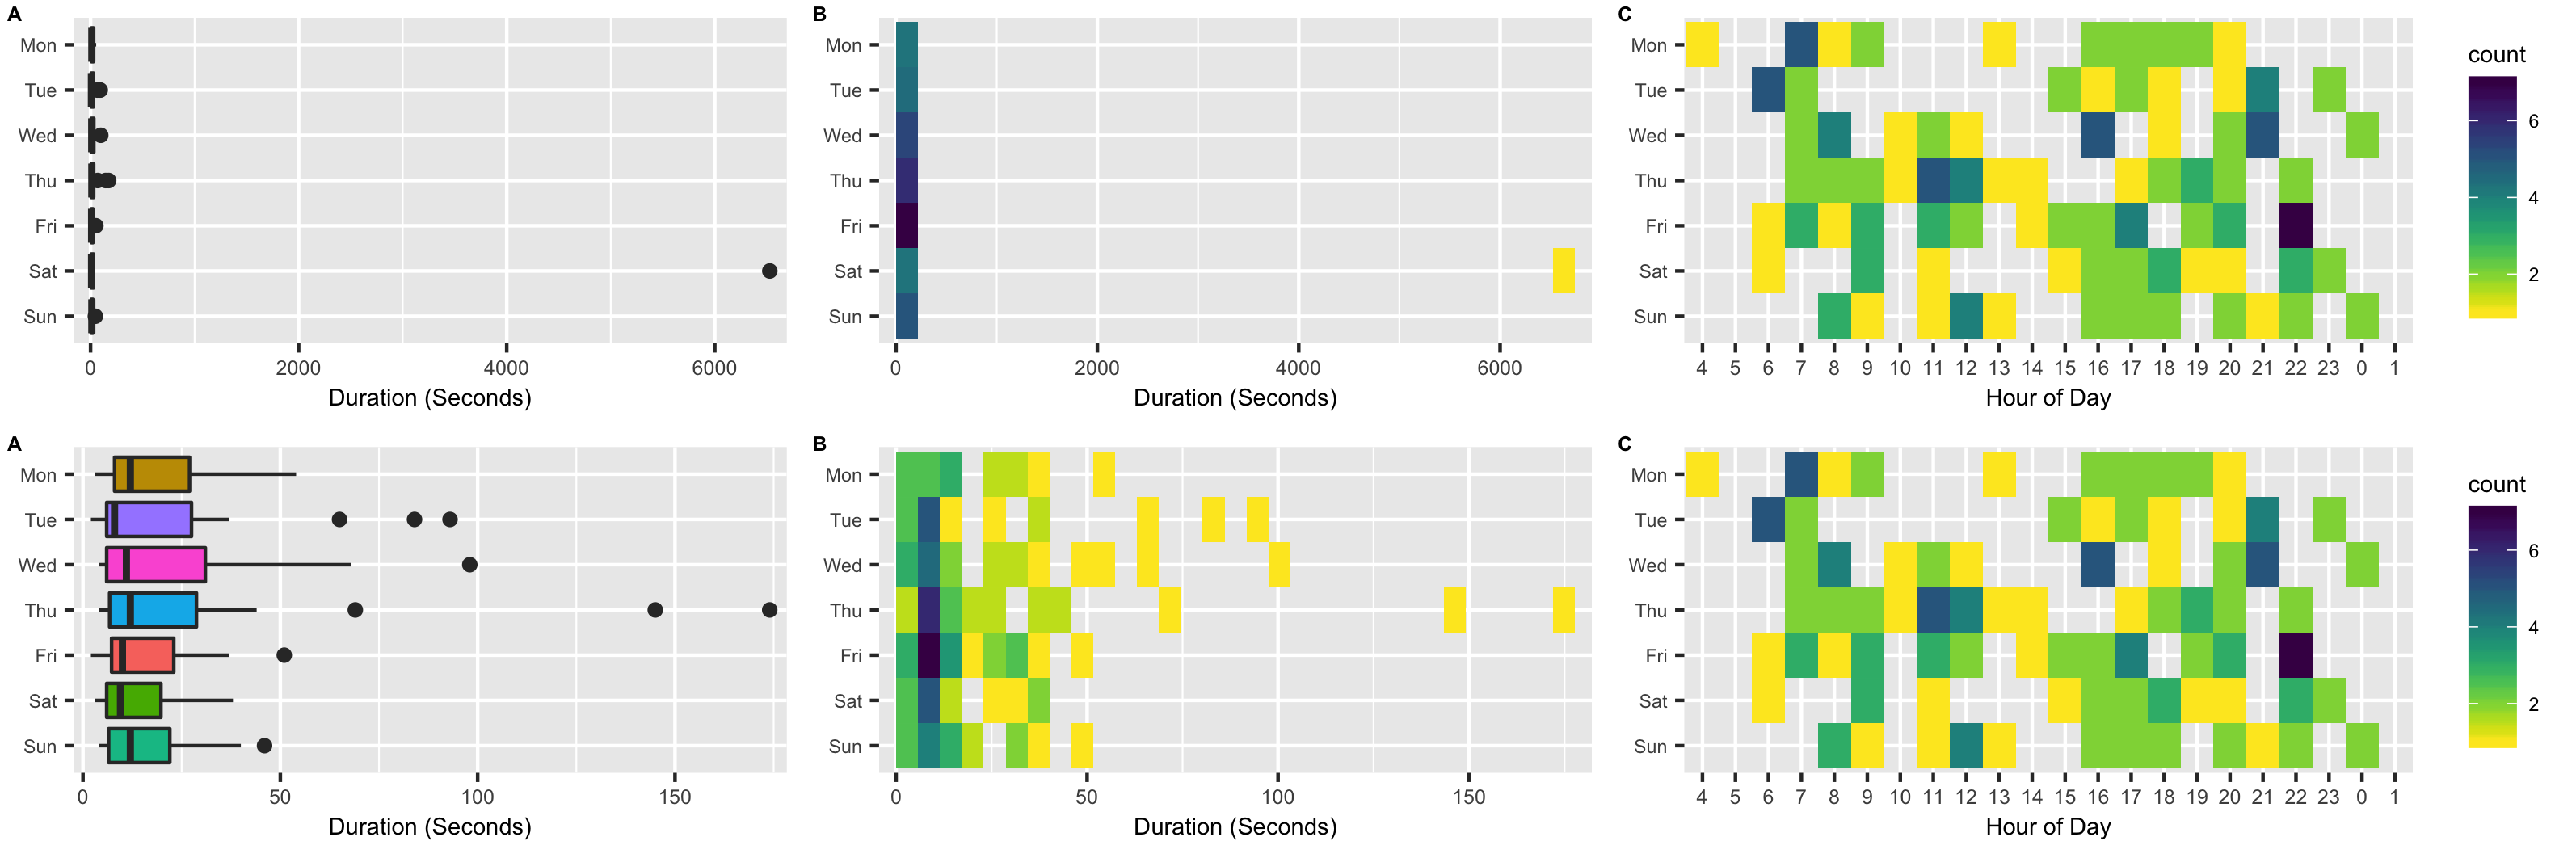
\includegraphics[width=1\linewidth]{/Users/alistairgj/Documents/GitHub/IoT_ResearchProject/IoT_November/images/subAct68} 

}

\caption{Initial and processed data box plot (A) and heat maps (B = day of week versus duration in seconds mapped by count, C = day of week versus hour of day mapped by count) for the Bathroom Sink Faucet sub activity.}\label{fig:subAct68}
\end{figure}

\hypertarget{kitchen-freezer---sub-activity-137}{%
\paragraph{Kitchen Freezer - Sub-Activity
137}\label{kitchen-freezer---sub-activity-137}}

The kitchen freezer has an overall count of n=130. Figure
\ref{fig:subAct137} boxplot (A) in row one shows many outliers on all
days but Monday, and abnormal results on Monday compared to the other
days. The median for this sub-activity is 39.0 seconds, and these
outliers are clearly outside the expected range for this sub-activity,
causing the mean to be 1738.11 seconds with a standard deviation of
4512.57 seconds. These outliers will be filled with the median (39.0
seconds). The resultant plots can be seen in the second row.

\begin{figure}[H]

{\centering 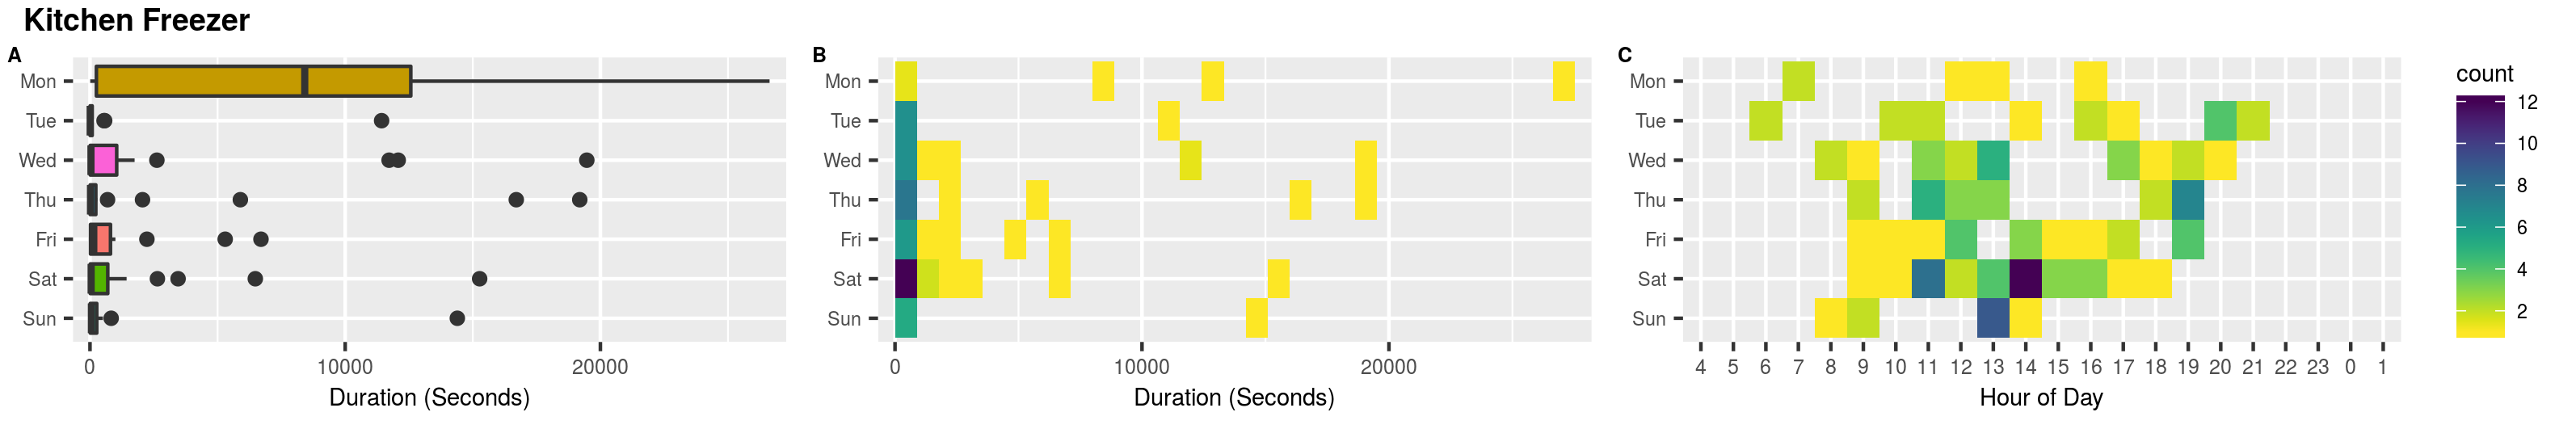
\includegraphics[width=1\linewidth]{/Users/alistairgj/Documents/GitHub/IoT_ResearchProject/IoT_November/images/subAct137} 

}

\caption{Initial and processed data box plot (A) and heat maps (B = day of week versus duration in seconds mapped by count, C = day of week versus hour of day mapped by count) for the Kitchen Freezer sub activity.}\label{fig:subAct137}
\end{figure}

\hypertarget{kitchen-lightswitch---sub-activity-105}{%
\paragraph{Kitchen Lightswitch - Sub-Activity
105}\label{kitchen-lightswitch---sub-activity-105}}

The kitchen lightswitch has an overall count of n=32. Figure
\ref{fig:subAct105} boxplot (A) in row one shows many abnormal results,
including one observation on Sunday at nearly 55,000 seconds, and
abnormally high results for Saturday when compared to the other days.
The median for this sub-activity is 4454.0 seconds, and many of these
results and outliers are clearly outside the expected range for this
sub-activity, causing the mean to be 9318.72 seconds with a standard
deviation of 13,081.34 seconds. The outliers will be filled with the
median (4454.0 seconds). The resultant plots can be seen in the second
row.

\begin{figure}[H]

{\centering 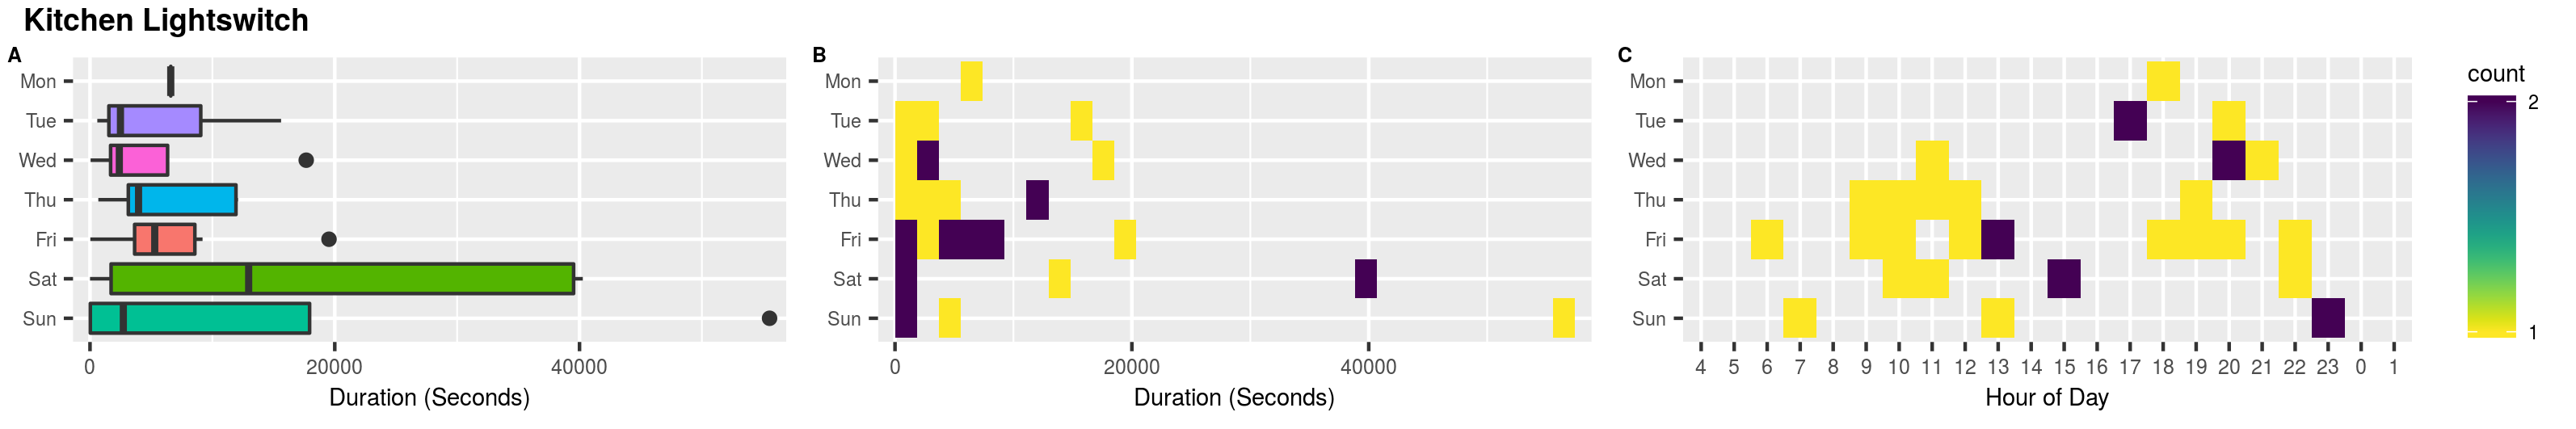
\includegraphics[width=1\linewidth]{/Users/alistairgj/Documents/GitHub/IoT_ResearchProject/IoT_November/images/subAct105} 

}

\caption{Initial and processed data box plot (A) and heat maps (B = day of week versus duration in seconds mapped by count, C = day of week versus hour of day mapped by count) for the Kitchen Lightswitch sub activity.}\label{fig:subAct105}
\end{figure}

\hypertarget{study-lightswitch---sub-activity-92}{%
\paragraph{Study Lightswitch - Sub-Activity
92}\label{study-lightswitch---sub-activity-92}}

The study lightswitch has an overall count of n=26. Figure
\ref{fig:subAct92} boxplot (A) in row one shows abnormal results for
Saturday and Sunday as compared to the other days. The median for this
sub-activity is 1728.5 seconds, and these abnormal results are clearly
outside the expected range for this sub-activity, causing the mean to be
6430.73 seconds with a standard deviation of 11,002.30 seconds. These
outliers will be filled with the median (1728.50 seconds). The resultant
plots can be seen in the second row.

\begin{figure}[H]

{\centering 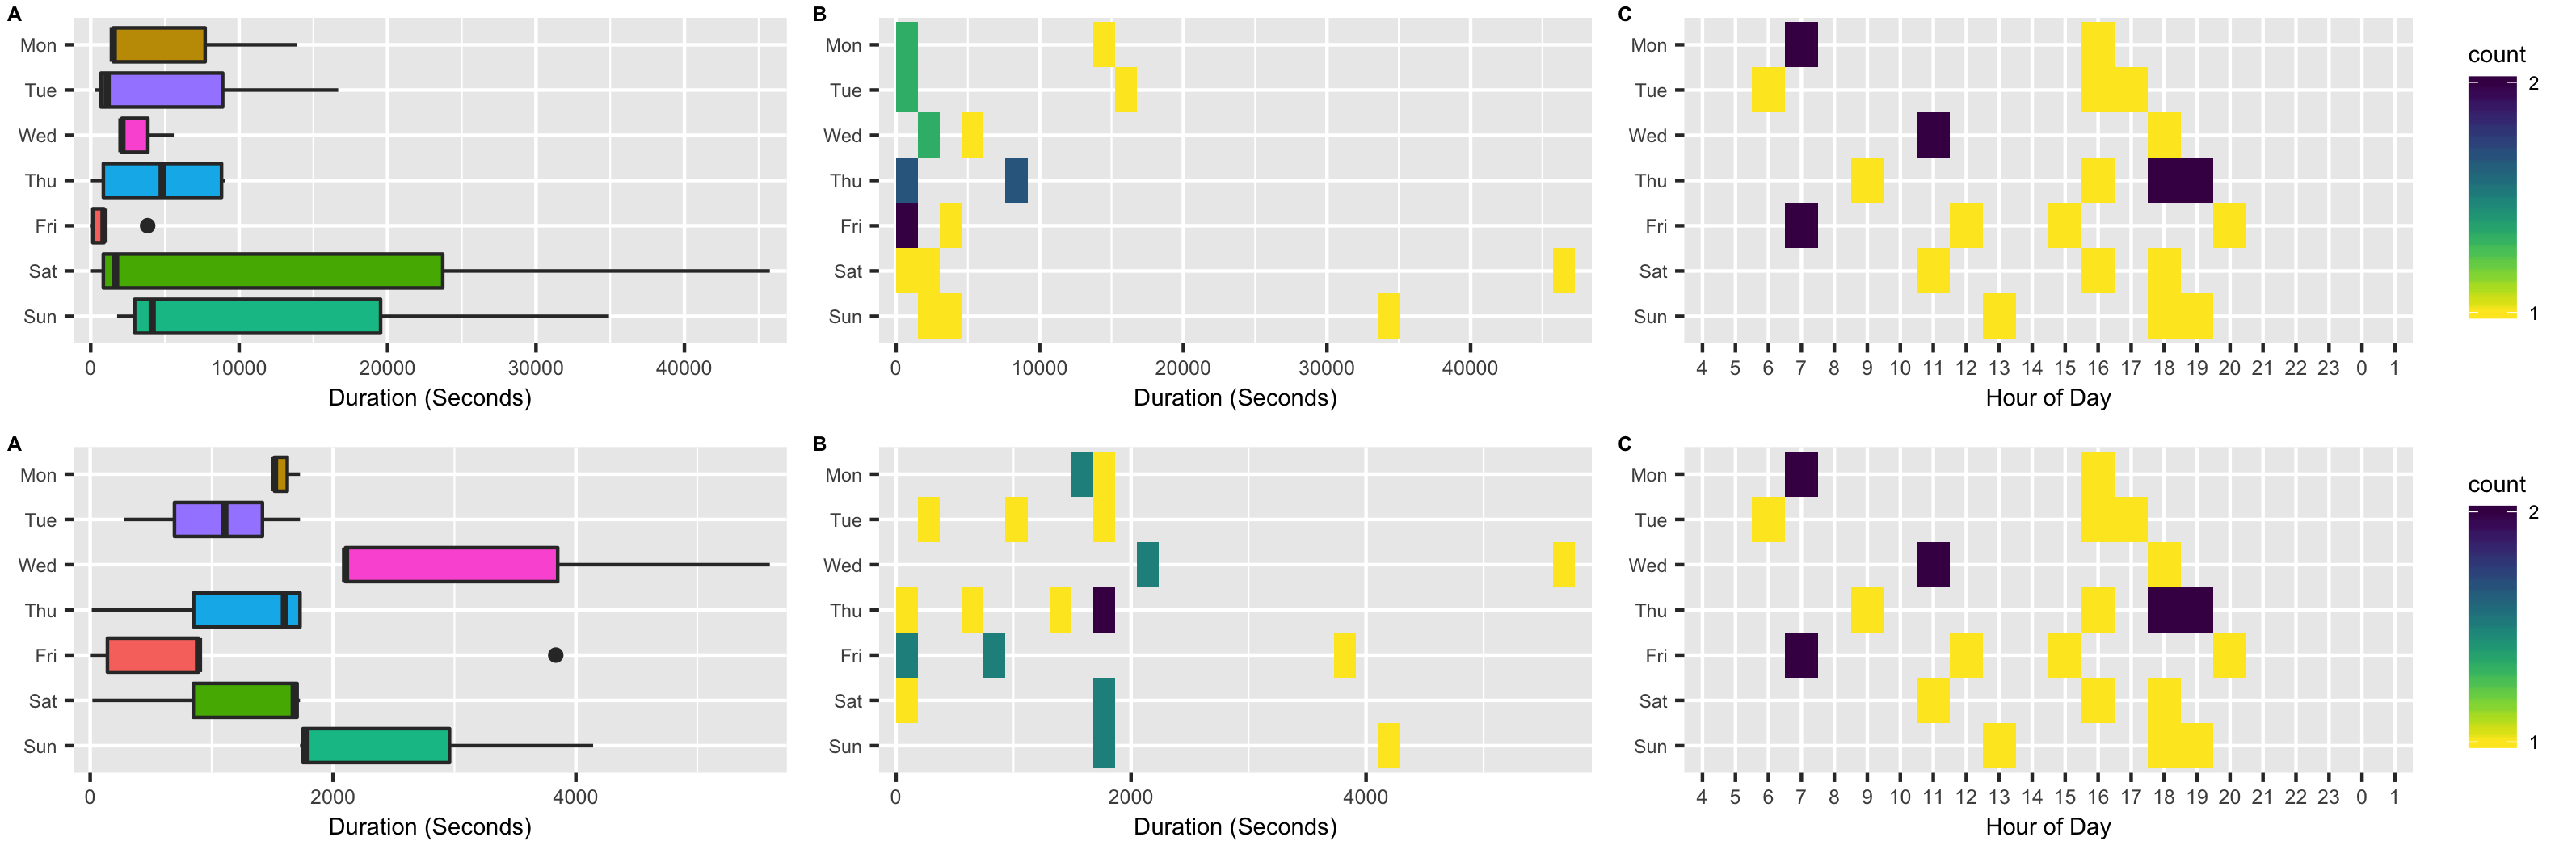
\includegraphics[width=1\linewidth]{/Users/alistairgj/Documents/GitHub/IoT_ResearchProject/IoT_November/images/subAct92} 

}

\caption{Initial and processed data box plot (A) and heat maps (B = day of week versus duration in seconds mapped by count, C = day of week versus hour of day mapped by count) for the Study Lightswitch sub-activity.}\label{fig:subAct92}
\end{figure}

\hypertarget{bathroom-door---sub-activity-130}{%
\paragraph{Bathroom Door - Sub-Activity
130}\label{bathroom-door---sub-activity-130}}

The bathroom door has an overall count of n=73. Figure
\ref{fig:subAct130} boxplot (A) in row one shows six extreme outliers,
with two of particular concern -- one on Thursday at around 10,000
seconds and one on Sunday at around 17,500 seconds. The median for this
sub-activity is 17.0 seconds, and these outliers are clearly outside the
expected range for this sub-activity, causing the mean to be 461.62
seconds with a standard deviation of 2310.81 seconds. These outliers
will be filled with the median (17.0 seconds). The resultant plots can
be seen in the second row.

\begin{figure}[H]

{\centering 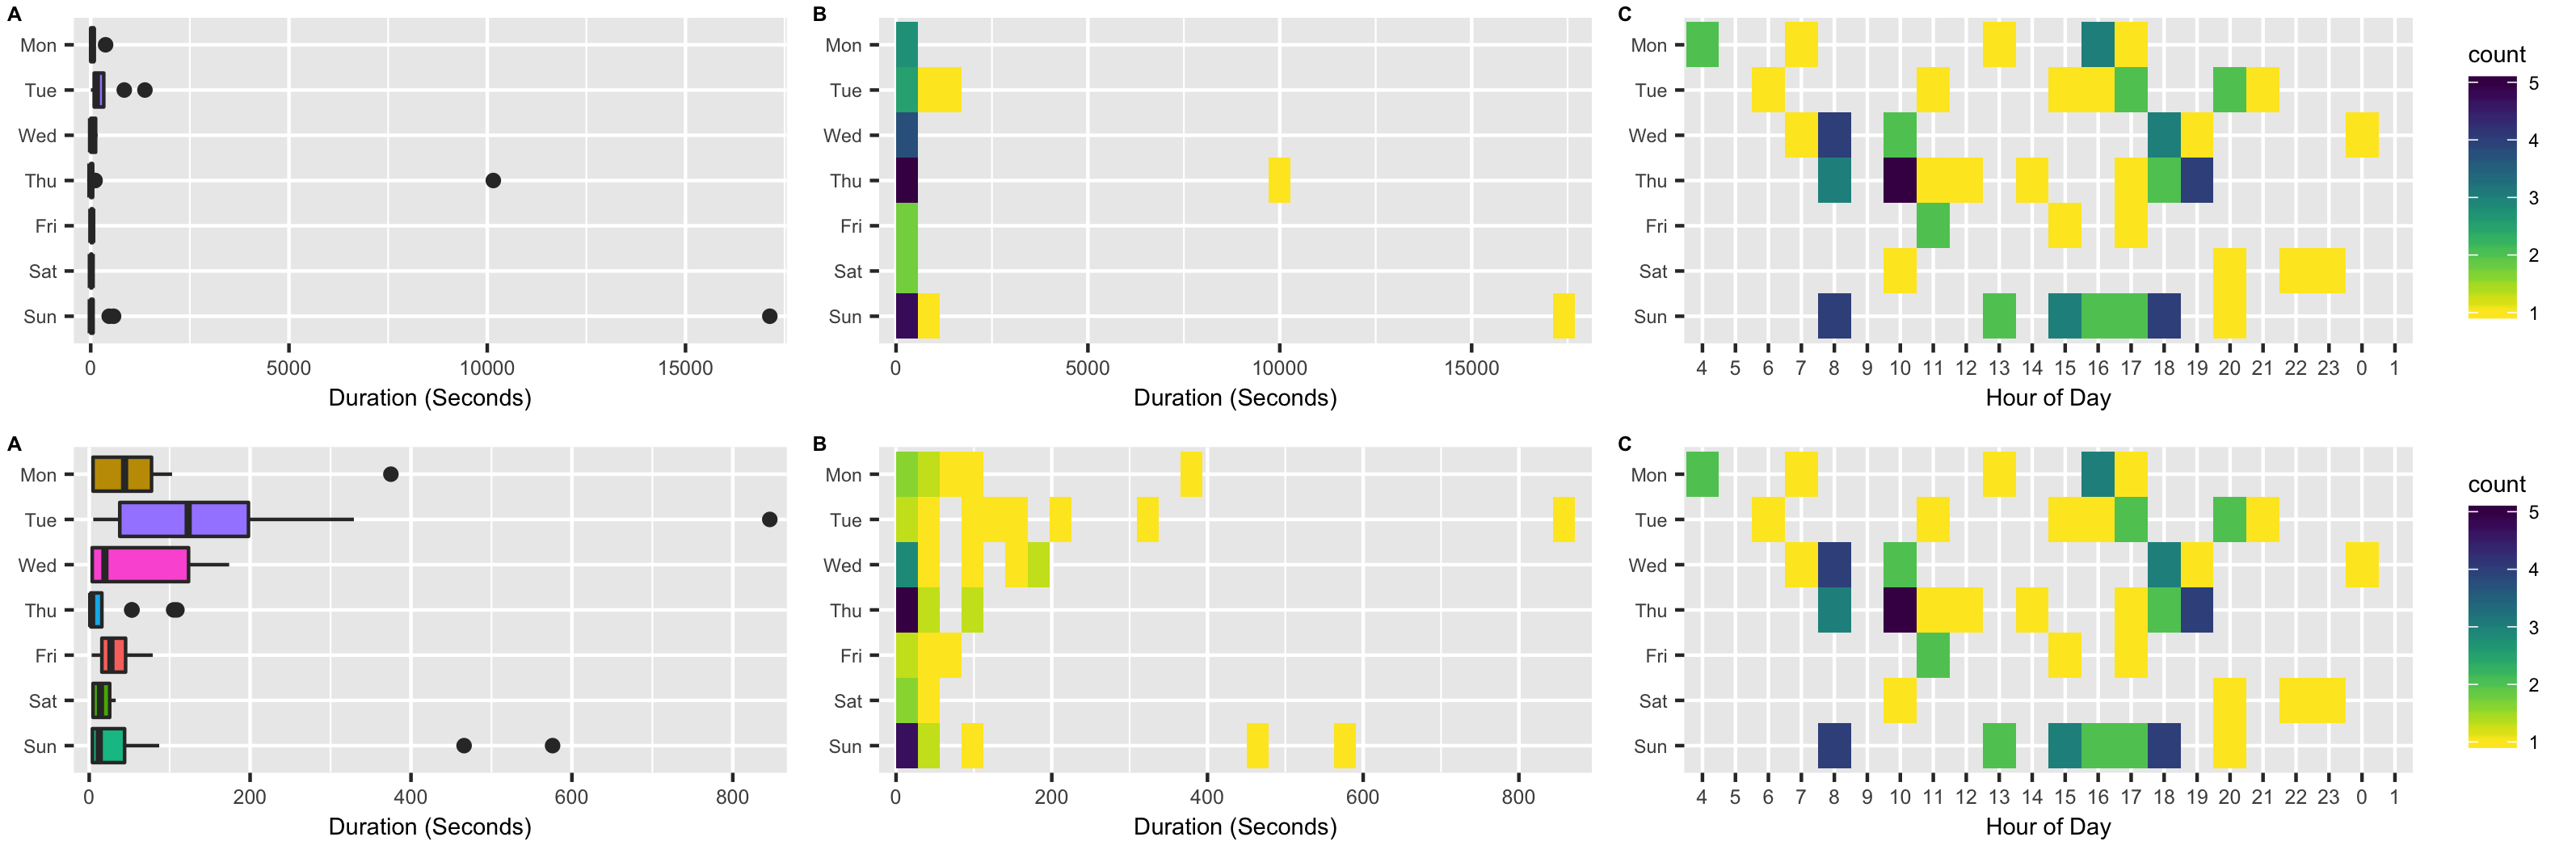
\includegraphics[width=1\linewidth]{/Users/alistairgj/Documents/GitHub/IoT_ResearchProject/IoT_November/images/subAct130} 

}

\caption{Initial and processed data box plot (A) and heat maps (B = day of week versus duration in seconds mapped by count, C = day of week versus hour of day mapped by count) for the Bathroom Door sub-activity.}\label{fig:subAct130}
\end{figure}

\hypertarget{kitchen-toaster---sub-activity-131}{%
\paragraph{Kitchen Toaster - Sub-Activity
131}\label{kitchen-toaster---sub-activity-131}}

The kitchen toaster has an overall count of n=71. Figure
\ref{fig:subAct131} boxplot (A) in row one shows two main extreme
outliers, one on Thursday at nearly 10,000 seconds and one on Friday at
nearly 30,000 seconds. There are also general abnormal results on Friday
as compared to the other days. The median for this sub-activity is 5.0
seconds, and these outliers and abnormal results are clearly outside the
expected range for this sub-activity, causing the mean to be 790.37
seconds with a standard deviation of 3793.67 seconds. These outliers and
abnormal results will be filled with the median (5.0 seconds). The
resultant plots can be seen in the second row.

\begin{figure}[H]

{\centering 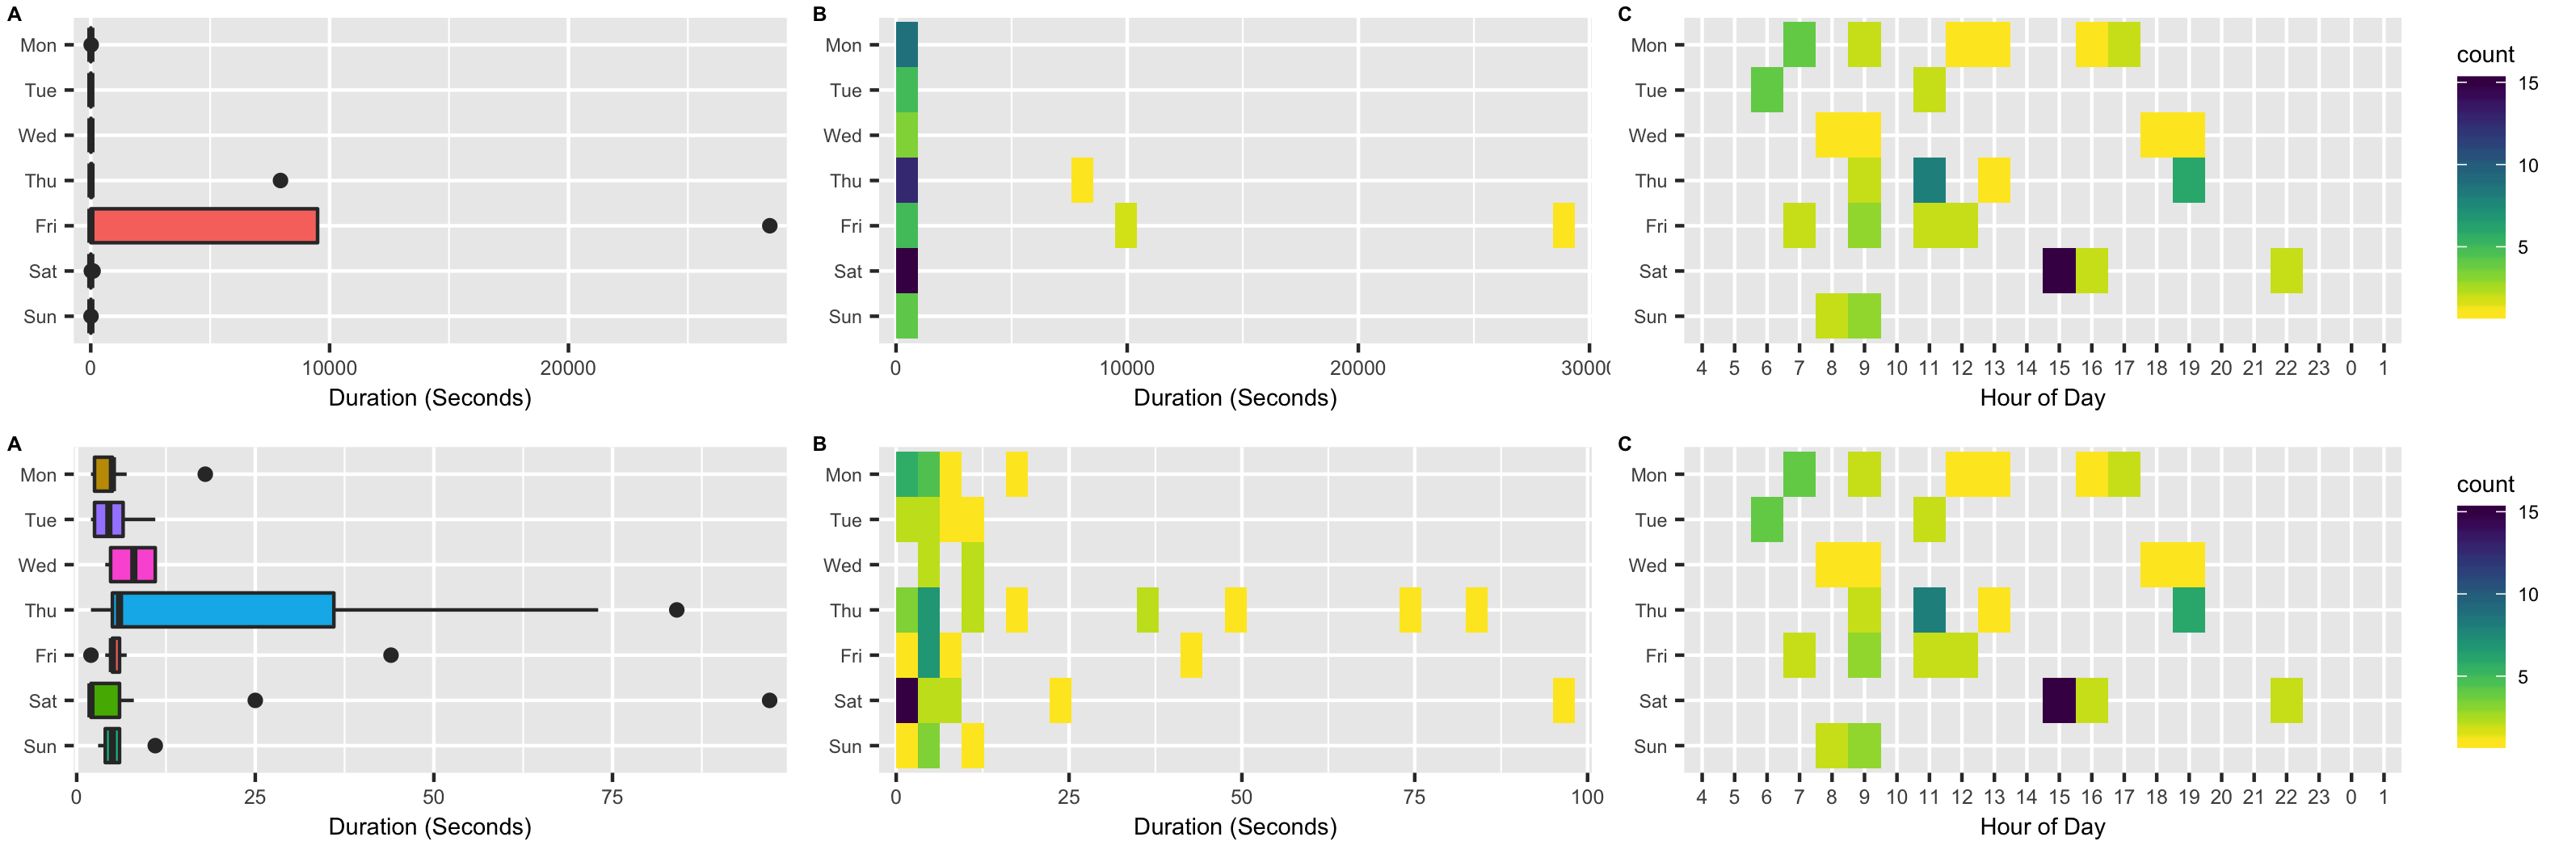
\includegraphics[width=1\linewidth]{/Users/alistairgj/Documents/GitHub/IoT_ResearchProject/IoT_November/images/subAct131} 

}

\caption{Initial and processed data box plot (A) and heat maps (B = day of week versus duration in seconds mapped by count, C = day of week versus hour of day mapped by count) for the Kitchen Toaster sub-activity.}\label{fig:subAct131}
\end{figure}

\hypertarget{livingroom-lightswitch---sub-activity-107}{%
\paragraph{Livingroom Lightswitch - Sub-Activity
107}\label{livingroom-lightswitch---sub-activity-107}}

The livingroom lightswitch has an overall count of n=8. Figure
\ref{fig:subAct107} boxplot (A) in row one shows variable results due to
the low count, with abnormally high results for Friday as compared to
the other days. The median for this sub-activity is 6352.5 seconds, with
a mean of 12,545.13 seconds and a standard deviation of 15,556.66
seconds. The abnormal values will be filled with the median (6352.50
seconds). The resultant plots can be seen in the second row.

\begin{figure}[H]

{\centering 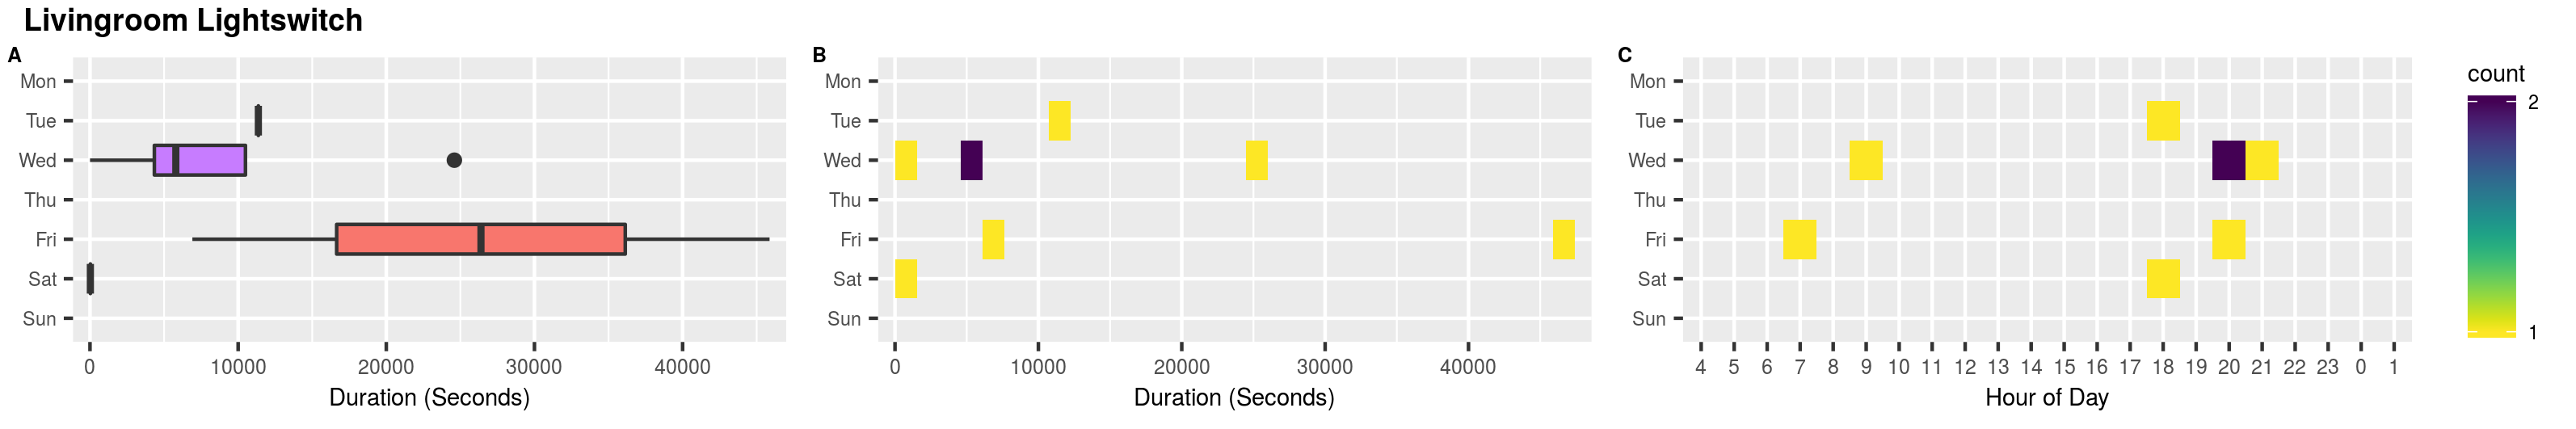
\includegraphics[width=1\linewidth]{/Users/alistairgj/Documents/GitHub/IoT_ResearchProject/IoT_November/images/subAct107} 

}

\caption{Initial and processed data box plot (A) and heat maps (B = day of week versus duration in seconds mapped by count, C = day of week versus hour of day mapped by count) for the Livingroom Lightswitch sub-activity.}\label{fig:subAct107}
\end{figure}

\hypertarget{foyer-closet---sub-activity-81}{%
\paragraph{Foyer Closet - Sub-Activity
81}\label{foyer-closet---sub-activity-81}}

The foyer closer has an overall count of n=29 in the dataset. In Figure
\ref{fig:subAct81} boxplot (A) in row one shows one key outlier just
under 1000 seconds. When considering all values together, the mean is
found to be 42.45 seconds, while the standard deviation is found to be
174.43 second. As the observation is so far from the median, it is
clearly having a large impact on the mean and standard deviation, and
the value of nearly 1000 seconds is unrealistic for the sub-activity in
question, the outlier will be filled with the median (8.0 seconds). The
resultant plots can be seen in the second row.

\begin{figure}[H]

{\centering 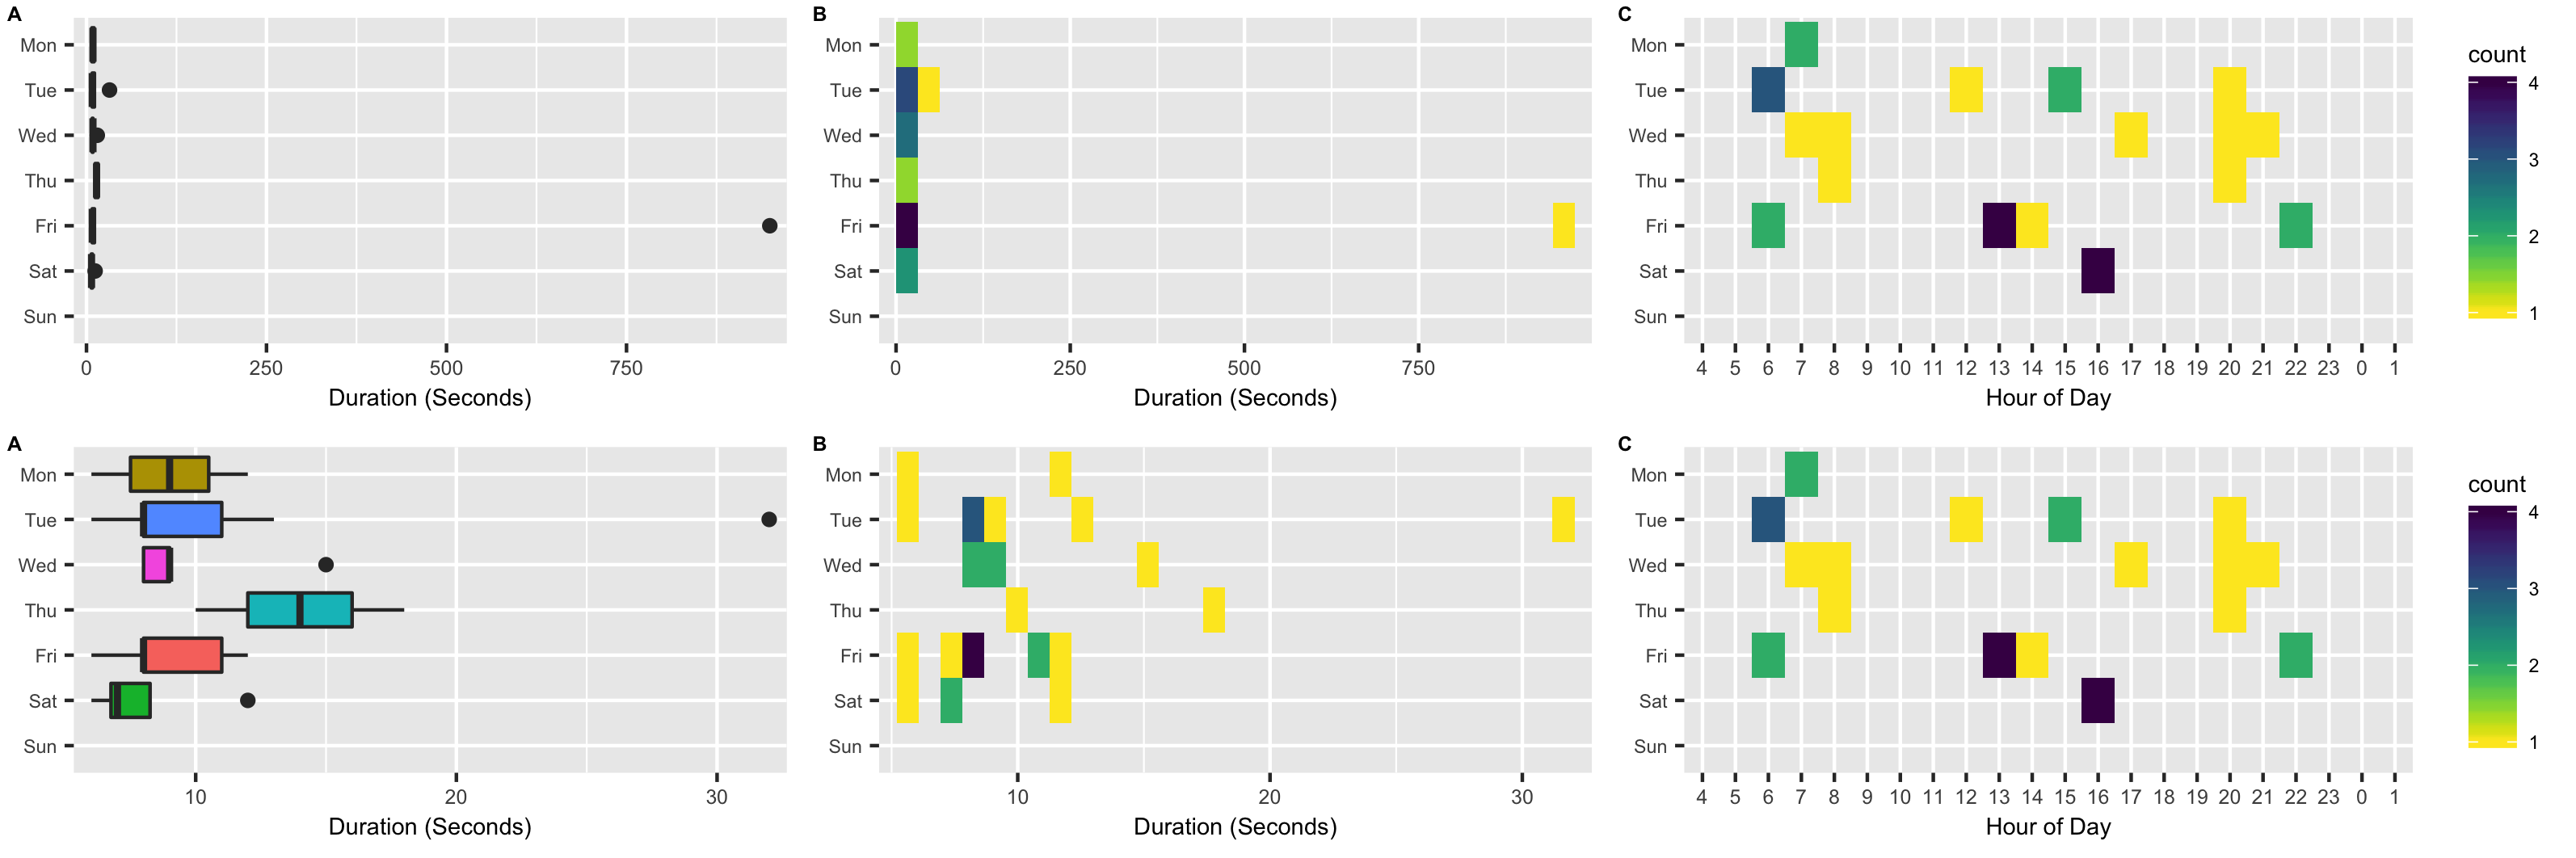
\includegraphics[width=1\linewidth]{/Users/alistairgj/Documents/GitHub/IoT_ResearchProject/IoT_November/images/subAct81} 

}

\caption{Initial and processed data box plot (A) and heat maps (B = day of week versus duration in seconds mapped by count, C = day of week versus hour of day mapped by count) for the Foyer Closet sub activity.}\label{fig:subAct81}
\end{figure}

\hypertarget{subactivity-cleansing---2-all-values-replaced-with-one-value}{%
\subsubsection{SubActivity Cleansing - 2) All values replaced with one
value}\label{subactivity-cleansing---2-all-values-replaced-with-one-value}}

This methodology was applied only to the bathroom toiletflush, with all
values being set to 1 second.

\hypertarget{bathroom-toiletflush---sub-activity-100}{%
\paragraph{Bathroom Toiletflush - Sub-Activity
100}\label{bathroom-toiletflush---sub-activity-100}}

Given the domain knowledge that it is unrealistic for a toilet flush to
last for thousands of seconds, and the lack of variability of the length
of toilet flushes, it was appropriate in this circumstance to presume
sensor or measurement error, and to replace the values instead with one
value -- 1 second. The initial (row one) and resultant (row two) plots
can be seen in Figure \ref{fig:subAct100}

\begin{figure}[H]

{\centering 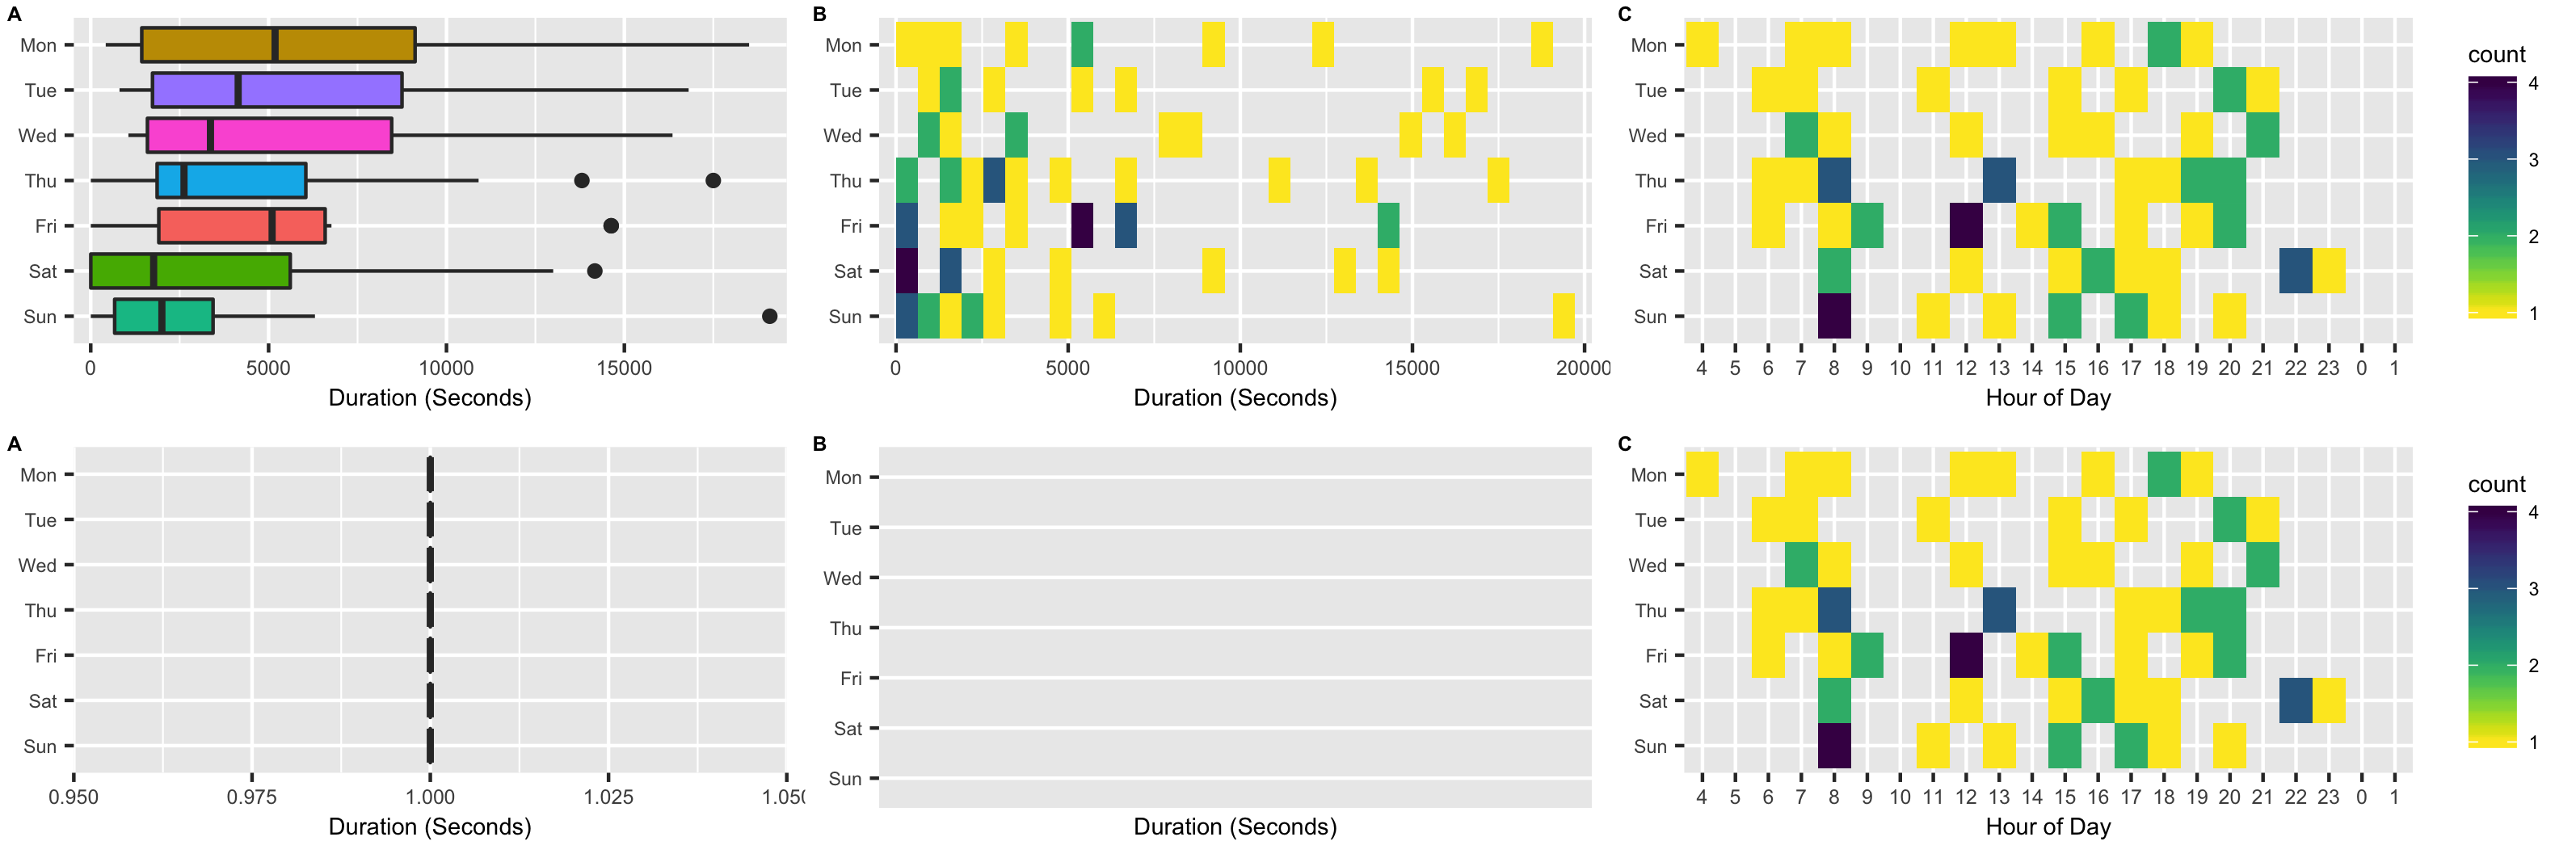
\includegraphics[width=1\linewidth]{/Users/alistairgj/Documents/GitHub/IoT_ResearchProject/IoT_November/images/subAct100} 

}

\caption{Initial and processed data box plot (A) and heat maps (B = day of week versus duration in seconds mapped by count, C = day of week versus hour of day mapped by count) for the bathroom toiletflush sub-activity.}\label{fig:subAct100}
\end{figure}

\hypertarget{subactivity-cleansing-review---3-no-futher-processing-required}{%
\subsubsection{SubActivity Cleansing Review - 3) No futher processing
required}\label{subactivity-cleansing-review---3-no-futher-processing-required}}

Based on the investigation of the box plots (A in all sub activity
plots), heat maps of day of week versus duration in seconds mapped by
count (B in all subactivity plots) and heat maps of day of week versus
hour of day mapped by count (C in all subactivity plots) the following
sub activities were left in their native state;
\texttt{bathroom\_lightswitch} (Figure \ref{fig:subAct101}, below),
\texttt{kitchen\_refrigerator} (Figure \ref{fig:subAct126}, below),
\texttt{bathroom\_sinkfaucet-cold} (Figure \ref{fig:subAct88}, below),
\texttt{foyer\_door} (Figure \ref{fig:subAct140}, below),
\texttt{kitchen\_burner} (Figure \ref{fig:subAct140}, below),
\texttt{foyer\_lightswitch} (Figure \ref{fig:subAct104}, below),
\texttt{bathroom\_exhaustfan} (Figure \ref{fig:subAct96}, below),
\texttt{bedroom\_lightswitch} (Figure \ref{fig:subAct108}, below),
\texttt{kitchen\_oven} (Figure \ref{fig:subAct129}, below),
\texttt{livingroom\_lamp} (Figure \ref{fig:subAct76}, below),
\texttt{kitchen\_washingmachine} (Figure \ref{fig:subAct142}, below),
\texttt{kitchen\_laundrydryer} (Figure \ref{fig:subAct90}, below),
\texttt{kitchen\_garbagedisposal} (Figure \ref{fig:subAct98}, below) and
\texttt{kitchen\_coffeemachine} (Figure \ref{fig:subAct119}, below).

\hypertarget{bathroom-lightswitch---sub-activity-101}{%
\paragraph{Bathroom Lightswitch - Sub-Activity
101}\label{bathroom-lightswitch---sub-activity-101}}

\begin{figure}[H]

{\centering 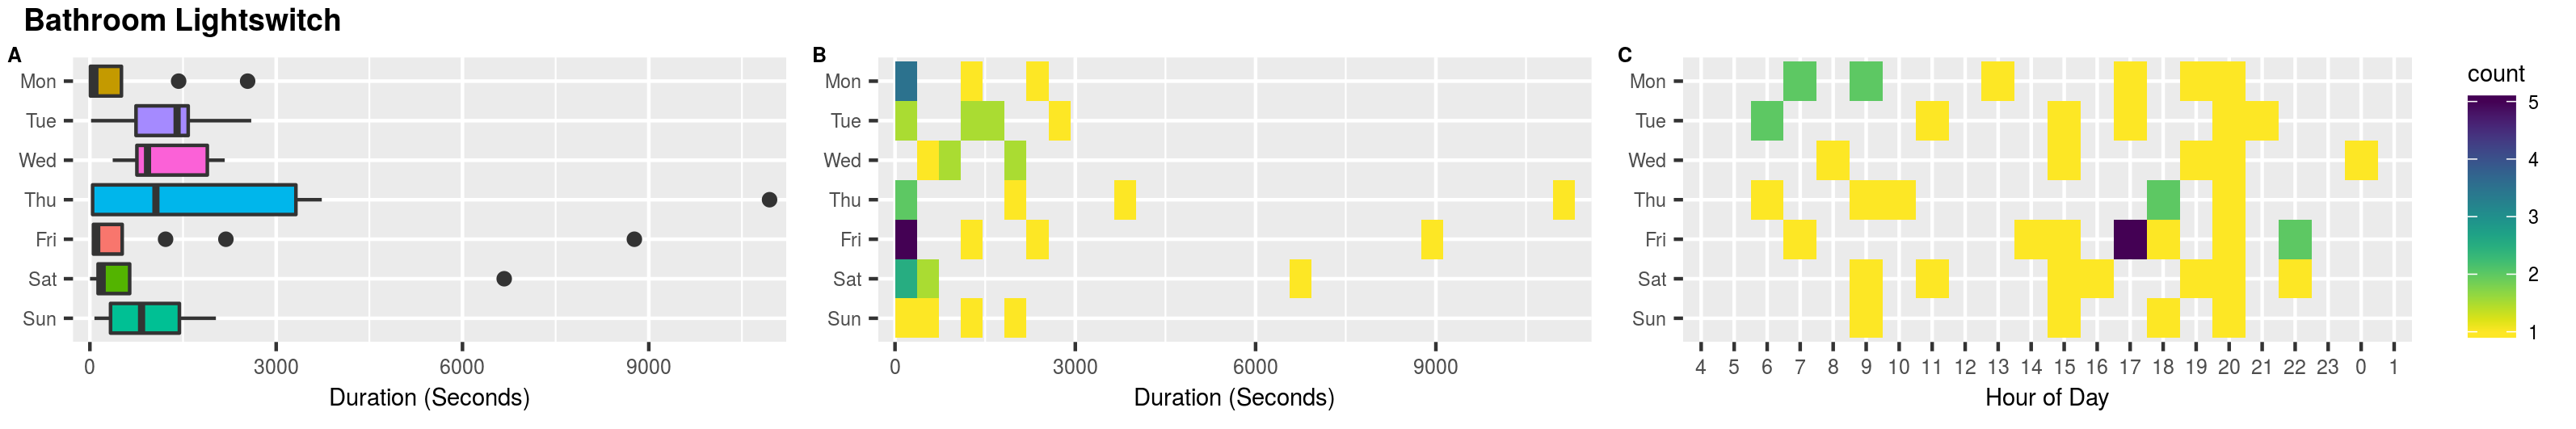
\includegraphics[width=1\linewidth]{/Users/alistairgj/Documents/GitHub/IoT_ResearchProject/IoT_November/images/subAct101} 

}

\caption{A caption}\label{fig:subAct101}
\end{figure}

\hypertarget{kitchen-refrigerator---sub-activity-126}{%
\paragraph{Kitchen Refrigerator - Sub-Activity
126}\label{kitchen-refrigerator---sub-activity-126}}

\begin{figure}[H]

{\centering 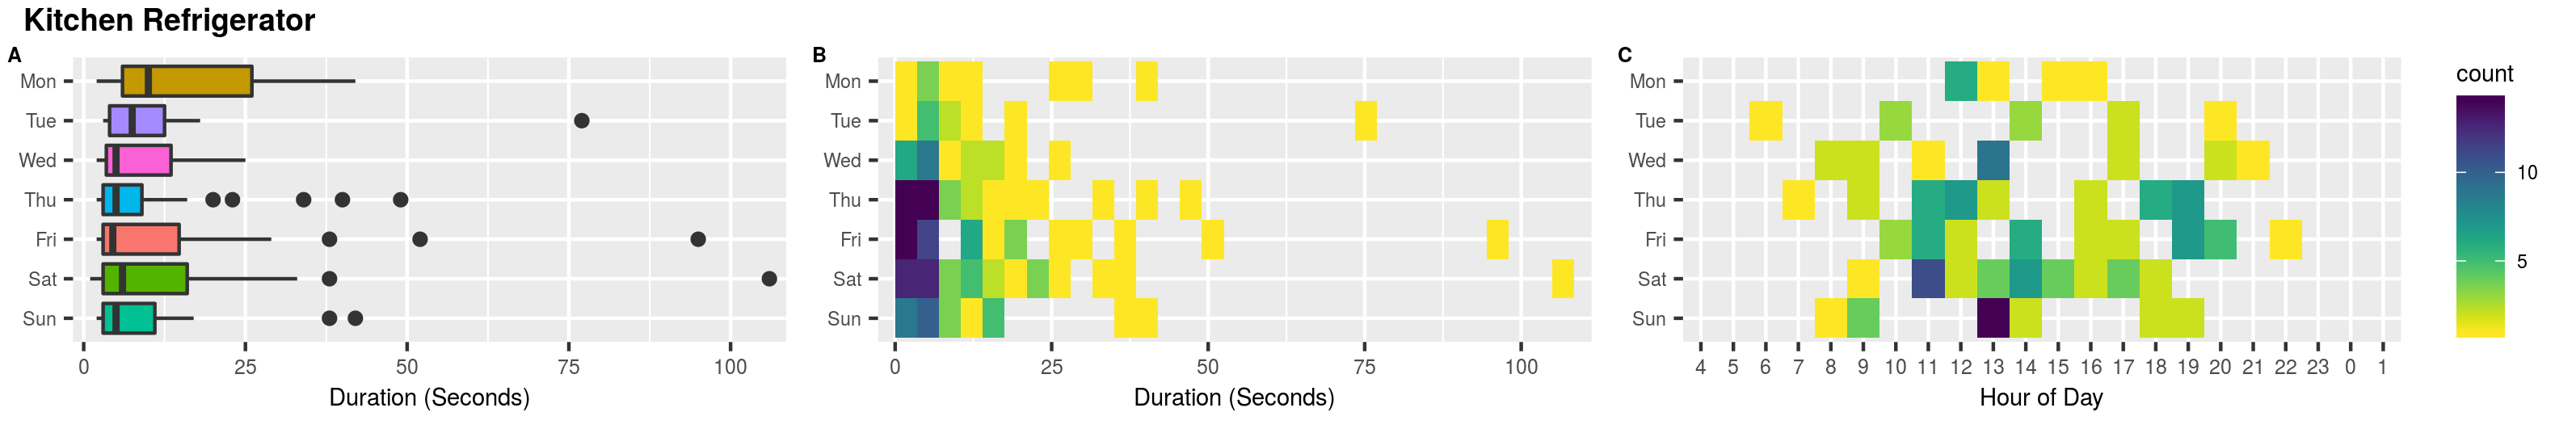
\includegraphics[width=1\linewidth]{/Users/alistairgj/Documents/GitHub/IoT_ResearchProject/IoT_November/images/subAct126} 

}

\caption{Box plot (A) and heat maps (B = day of week versus duration in seconds mapped by count, C = day of week versus hour of day mapped by count) for the Kitchen Refrigerator sub activity.}\label{fig:subAct126}
\end{figure}

\hypertarget{bathroom-sink-faucet-cold---sub-activity-88}{%
\paragraph{Bathroom Sink Faucet (Cold) - Sub-Activity
88}\label{bathroom-sink-faucet-cold---sub-activity-88}}

\begin{figure}[H]

{\centering 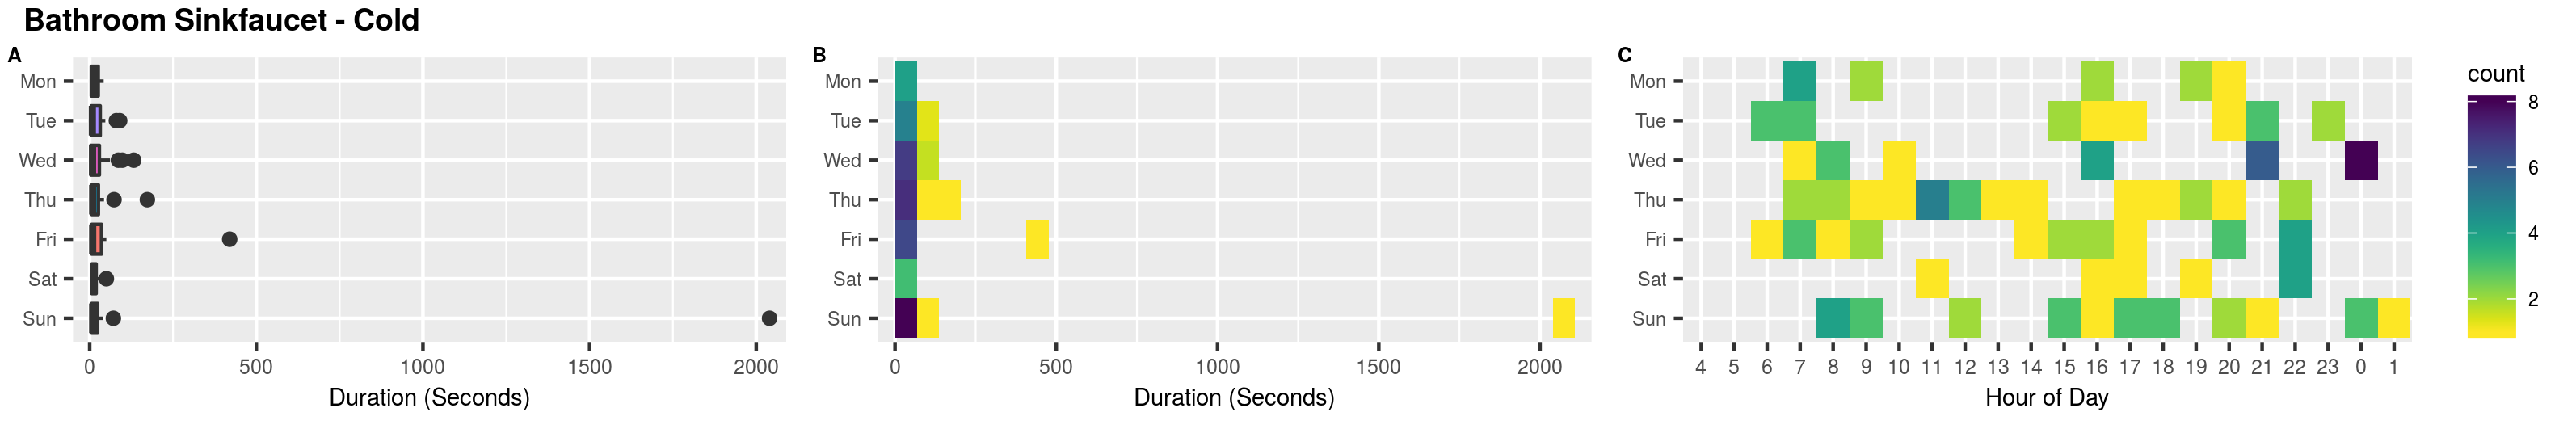
\includegraphics[width=1\linewidth]{/Users/alistairgj/Documents/GitHub/IoT_ResearchProject/IoT_November/images/subAct88} 

}

\caption{Box plot (A) and heat maps (B = day of week versus duration in seconds mapped by count, C = day of week versus hour of day mapped by count) for the Bathroom sick faucted - cold sub-activity.}\label{fig:subAct88}
\end{figure}

\hypertarget{foyer-door---sub-activity-140}{%
\paragraph{Foyer Door - Sub-Activity
140}\label{foyer-door---sub-activity-140}}

\begin{figure}[H]

{\centering 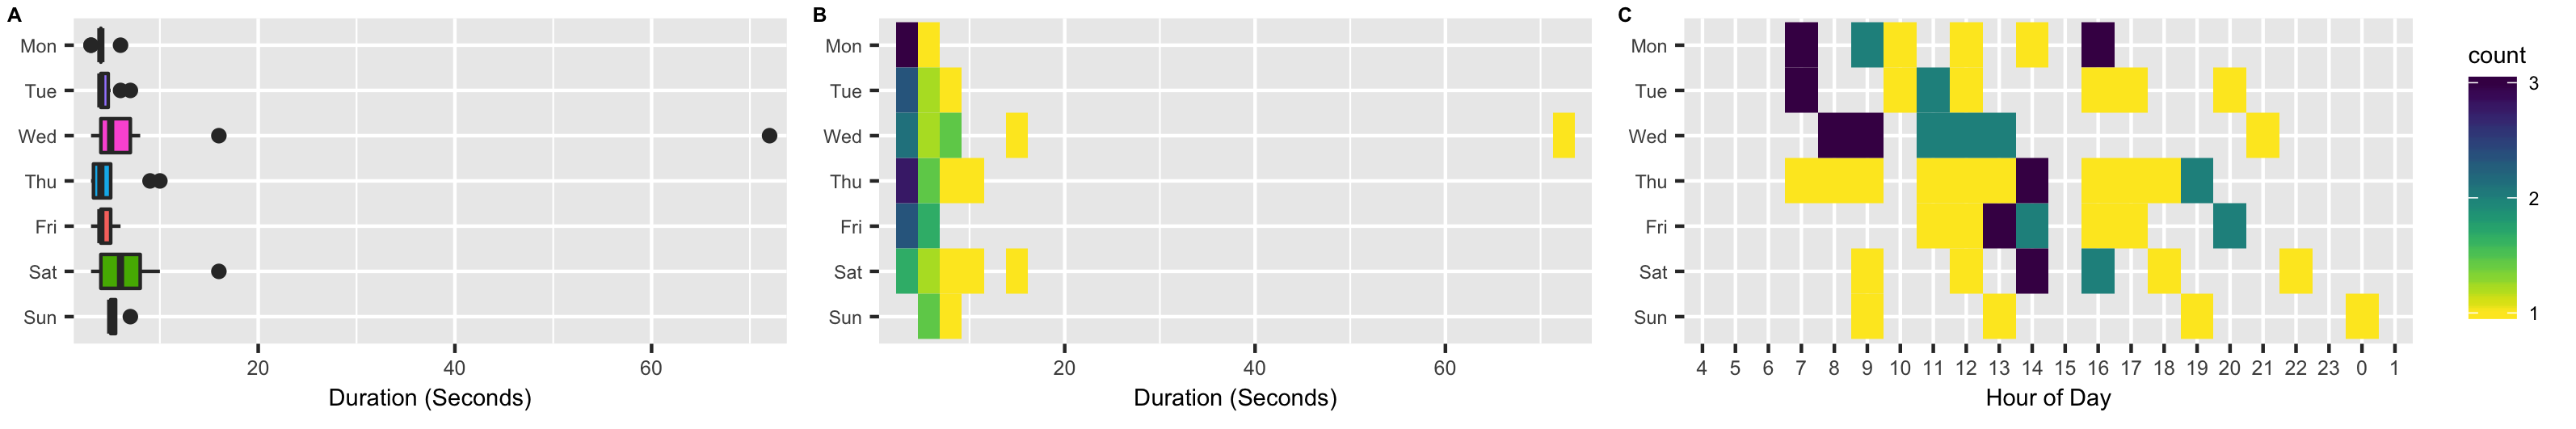
\includegraphics[width=1\linewidth]{/Users/alistairgj/Documents/GitHub/IoT_ResearchProject/IoT_November/images/subAct140} 

}

\caption{Box plot (A) and heat maps (B = day of week versus duration in seconds mapped by count, C = day of week versus hour of day mapped by count) for the Foyer Door sub-activity.}\label{fig:subAct140}
\end{figure}

\hypertarget{kitchen-burner---sub-activity-140}{%
\paragraph{Kitchen Burner - Sub-Activity
140}\label{kitchen-burner---sub-activity-140}}

\begin{figure}[H]

{\centering 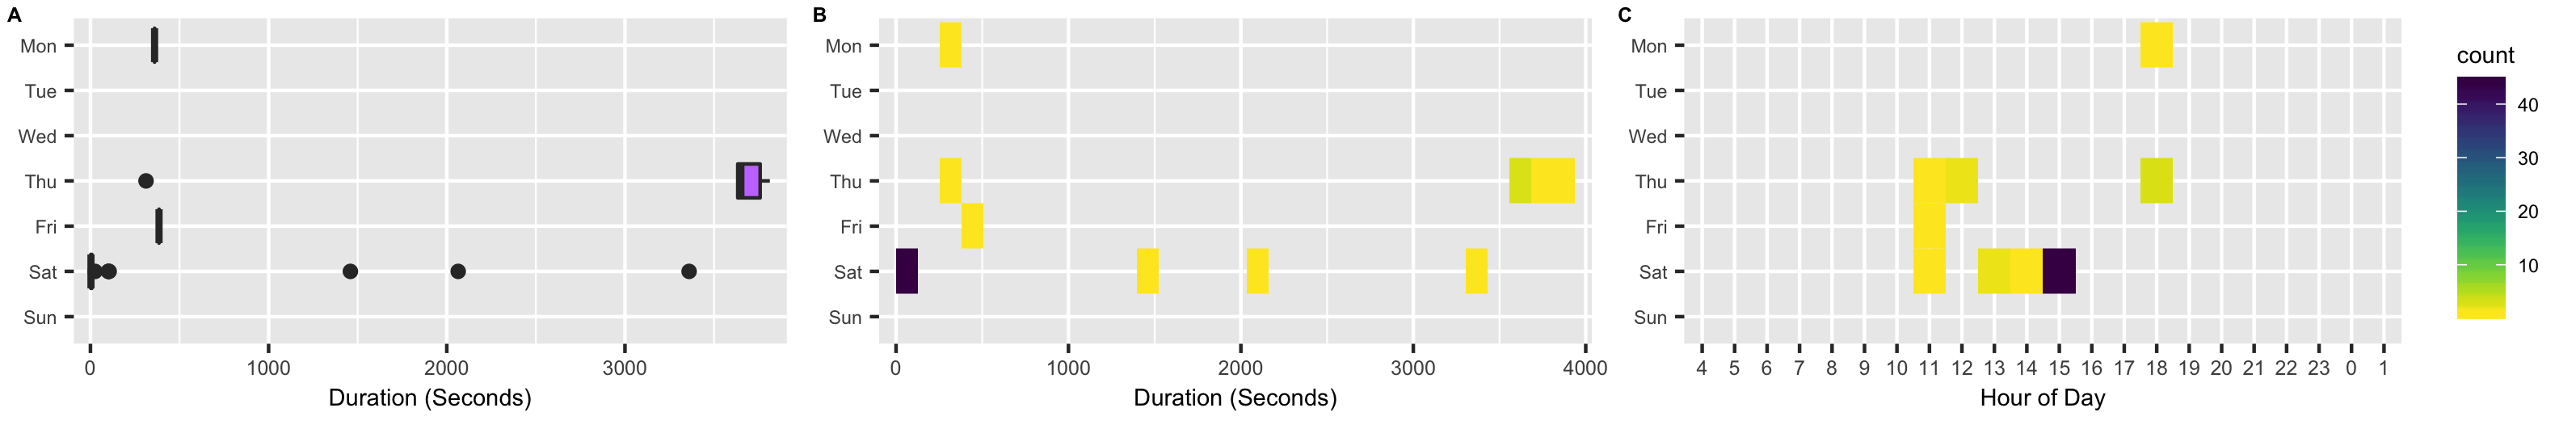
\includegraphics[width=1\linewidth]{/Users/alistairgj/Documents/GitHub/IoT_ResearchProject/IoT_November/images/subAct106} 

}

\caption{Box plot (A) and heat maps (B = day of week versus duration in seconds mapped by count, C = day of week versus hour of day mapped by count) for the Kitchen Burner sub-activity.}\label{fig:subAct106}
\end{figure}

\hypertarget{foyer-lightswitch---sub-activity-104}{%
\paragraph{Foyer Lightswitch - Sub-Activity
104}\label{foyer-lightswitch---sub-activity-104}}

\begin{figure}[H]

{\centering 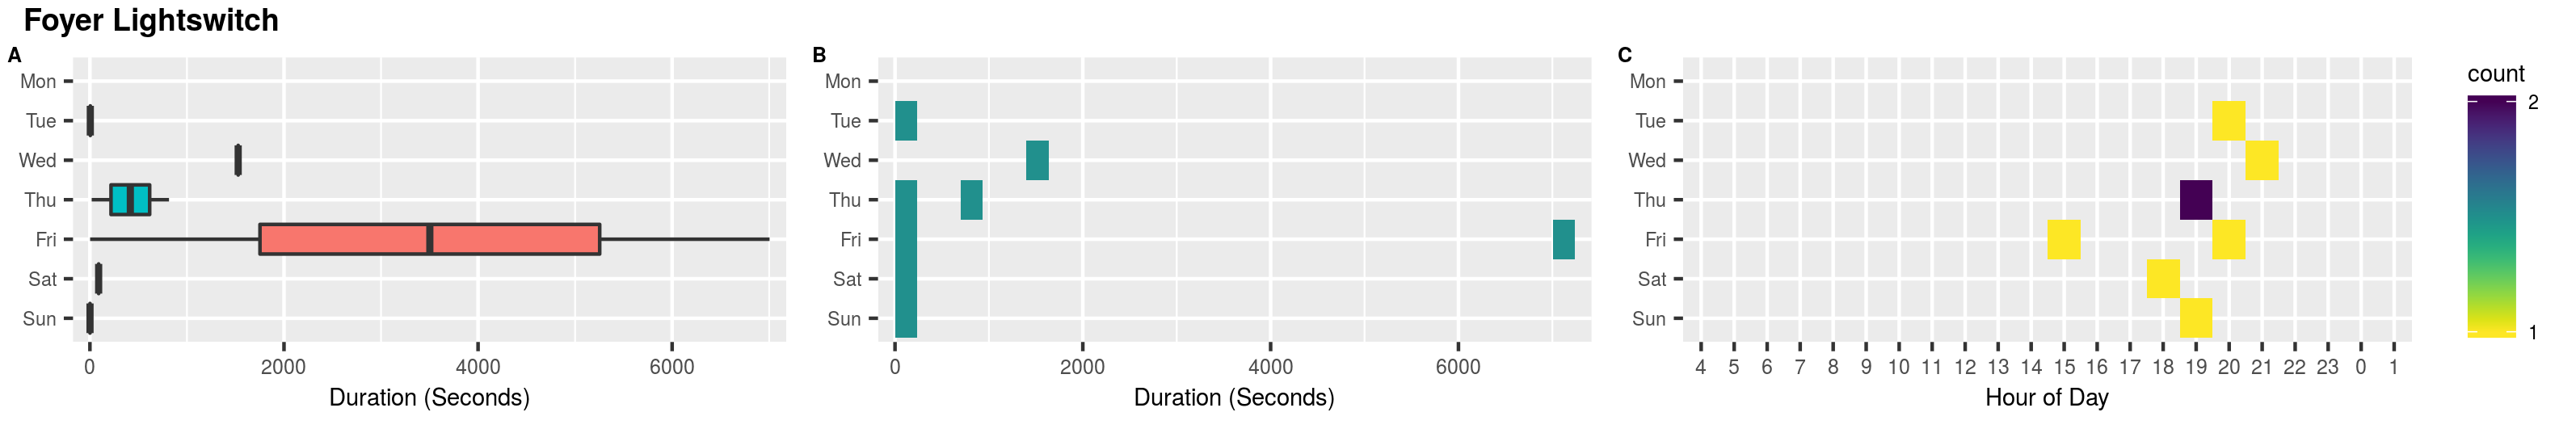
\includegraphics[width=1\linewidth]{/Users/alistairgj/Documents/GitHub/IoT_ResearchProject/IoT_November/images/subAct104} 

}

\caption{Box plot (A) and heat maps (B = day of week versus duration in seconds mapped by count, C = day of week versus hour of day mapped by count) for the Foyer Lightswitch sub-activity.}\label{fig:subAct104}
\end{figure}

\hypertarget{bathroom-exhaust-fan---sub-activity-96}{%
\paragraph{Bathroom Exhaust Fan - Sub-Activity
96}\label{bathroom-exhaust-fan---sub-activity-96}}

\begin{figure}[H]

{\centering 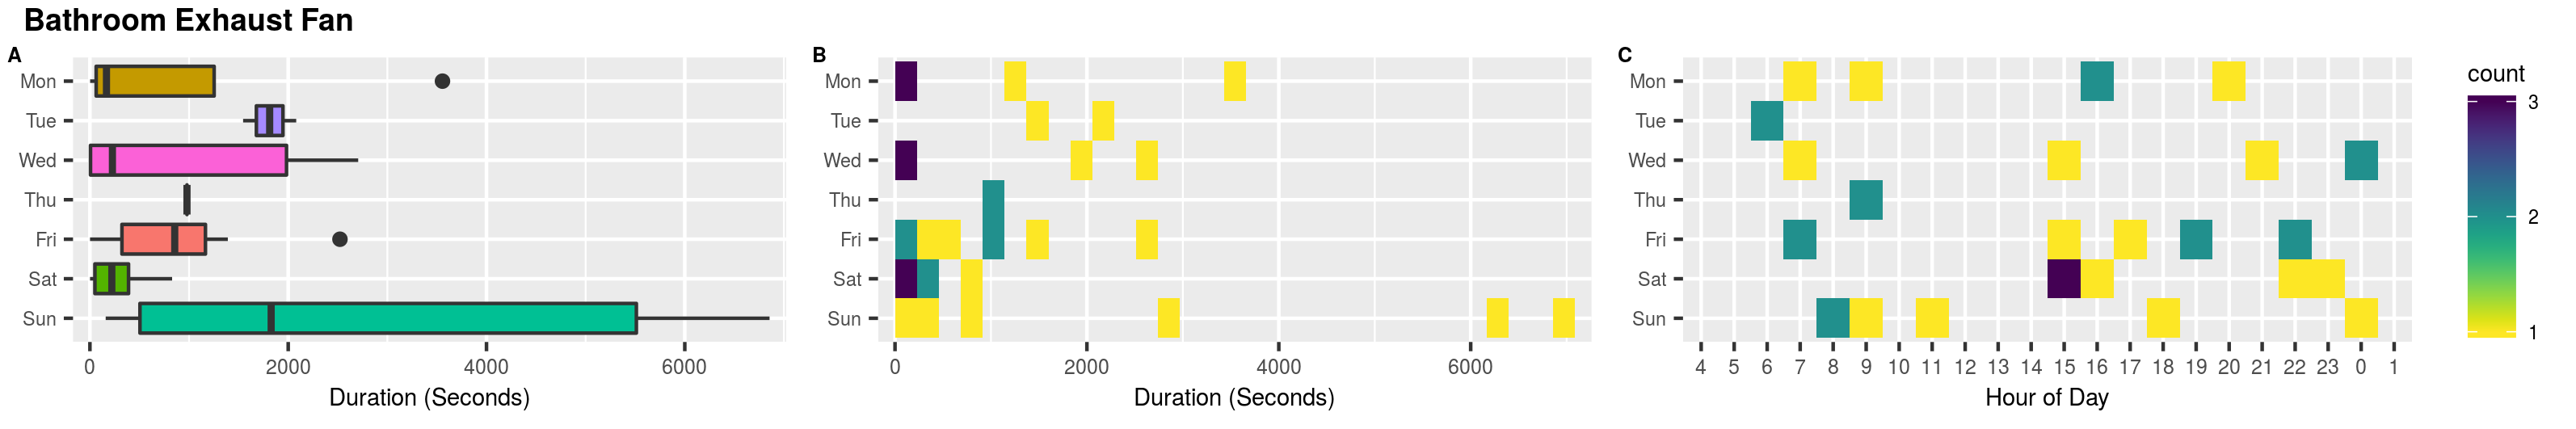
\includegraphics[width=1\linewidth]{/Users/alistairgj/Documents/GitHub/IoT_ResearchProject/IoT_November/images/subAct96} 

}

\caption{Box plot (A) and heat maps (B = day of week versus duration in seconds mapped by count, C = day of week versus hour of day mapped by count) for the Bathroom Exhaust Fan sub-activity.}\label{fig:subAct96}
\end{figure}

\hypertarget{bedroom-lightswitch---sub-activity-108}{%
\paragraph{Bedroom Lightswitch - Sub-Activity
108}\label{bedroom-lightswitch---sub-activity-108}}

\begin{figure}[H]

{\centering 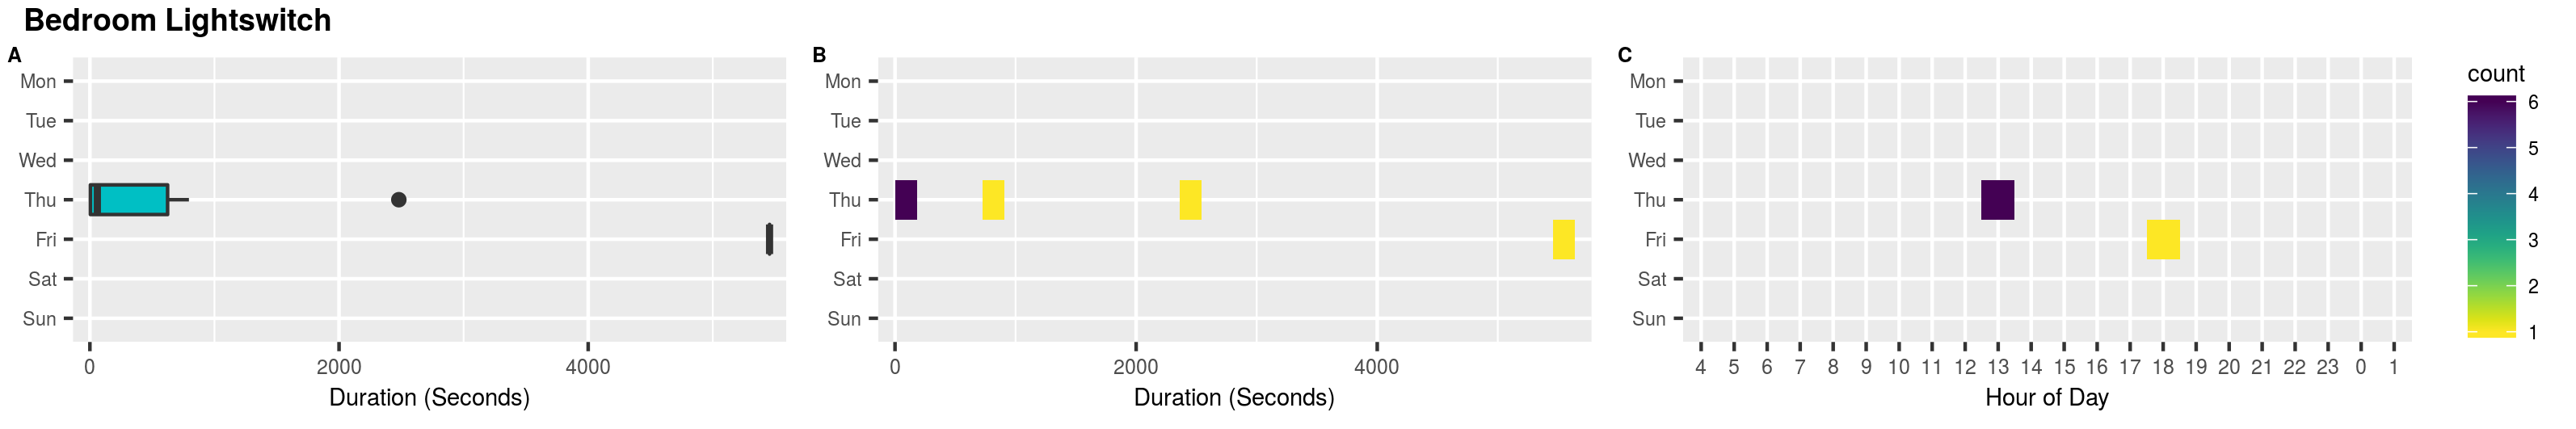
\includegraphics[width=1\linewidth]{/Users/alistairgj/Documents/GitHub/IoT_ResearchProject/IoT_November/images/subAct108} 

}

\caption{Box plot (A) and heat maps (B = day of week versus duration in seconds mapped by count, C = day of week versus hour of day mapped by count) for the Bedroom Lightswitch sub-activity.}\label{fig:subAct108}
\end{figure}

\hypertarget{kitchen-oven---sub-activity-129}{%
\paragraph{Kitchen Oven - Sub-Activity
129}\label{kitchen-oven---sub-activity-129}}

\begin{figure}[H]

{\centering 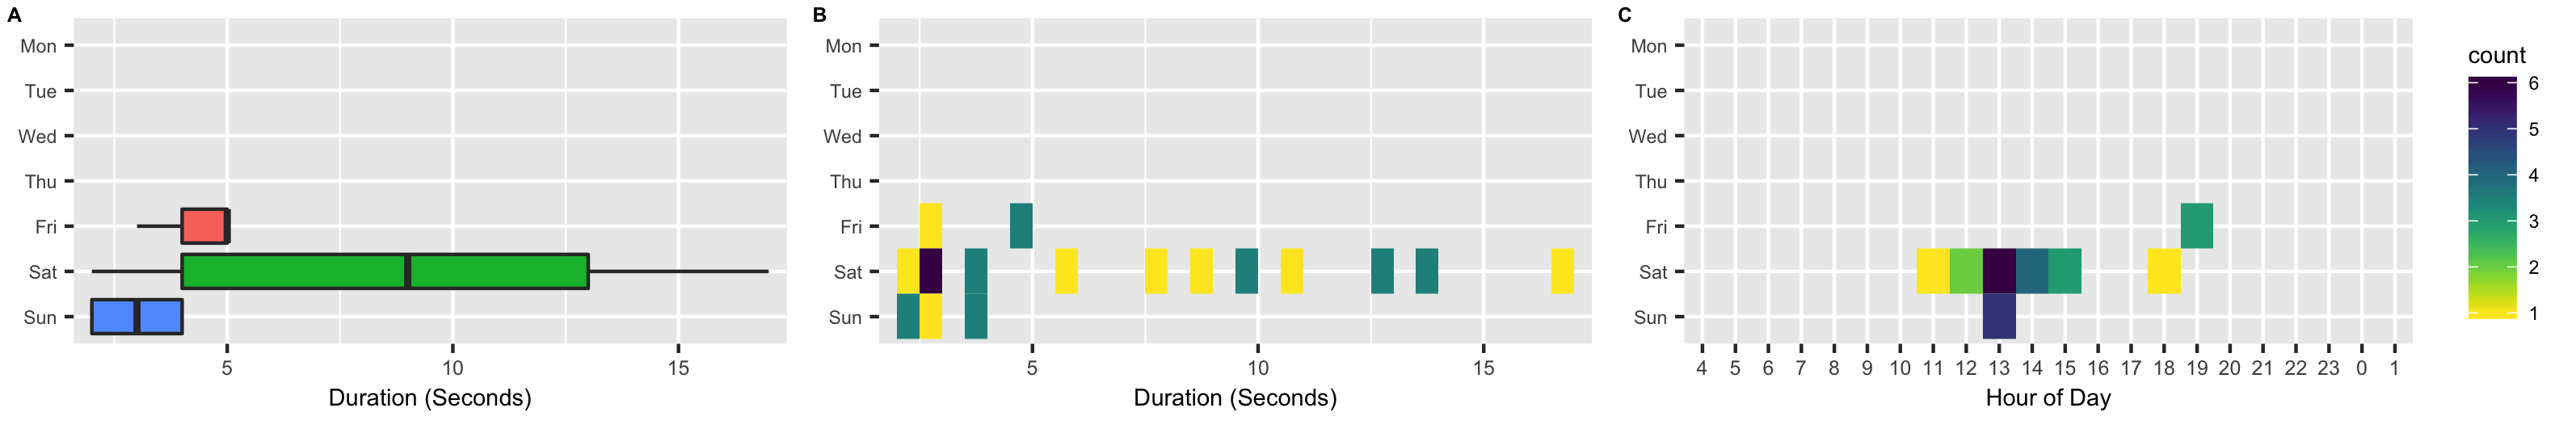
\includegraphics[width=1\linewidth]{/Users/alistairgj/Documents/GitHub/IoT_ResearchProject/IoT_November/images/subAct129} 

}

\caption{Box plot (A) and heat maps (B = day of week versus duration in seconds mapped by count, C = day of week versus hour of day mapped by count) for the Kitchen Oven sub-activity.}\label{fig:subAct129}
\end{figure}

\hypertarget{livingroom-lamp---sub-activity-76}{%
\paragraph{Livingroom Lamp - Sub-Activity
76}\label{livingroom-lamp---sub-activity-76}}

\begin{figure}[H]

{\centering 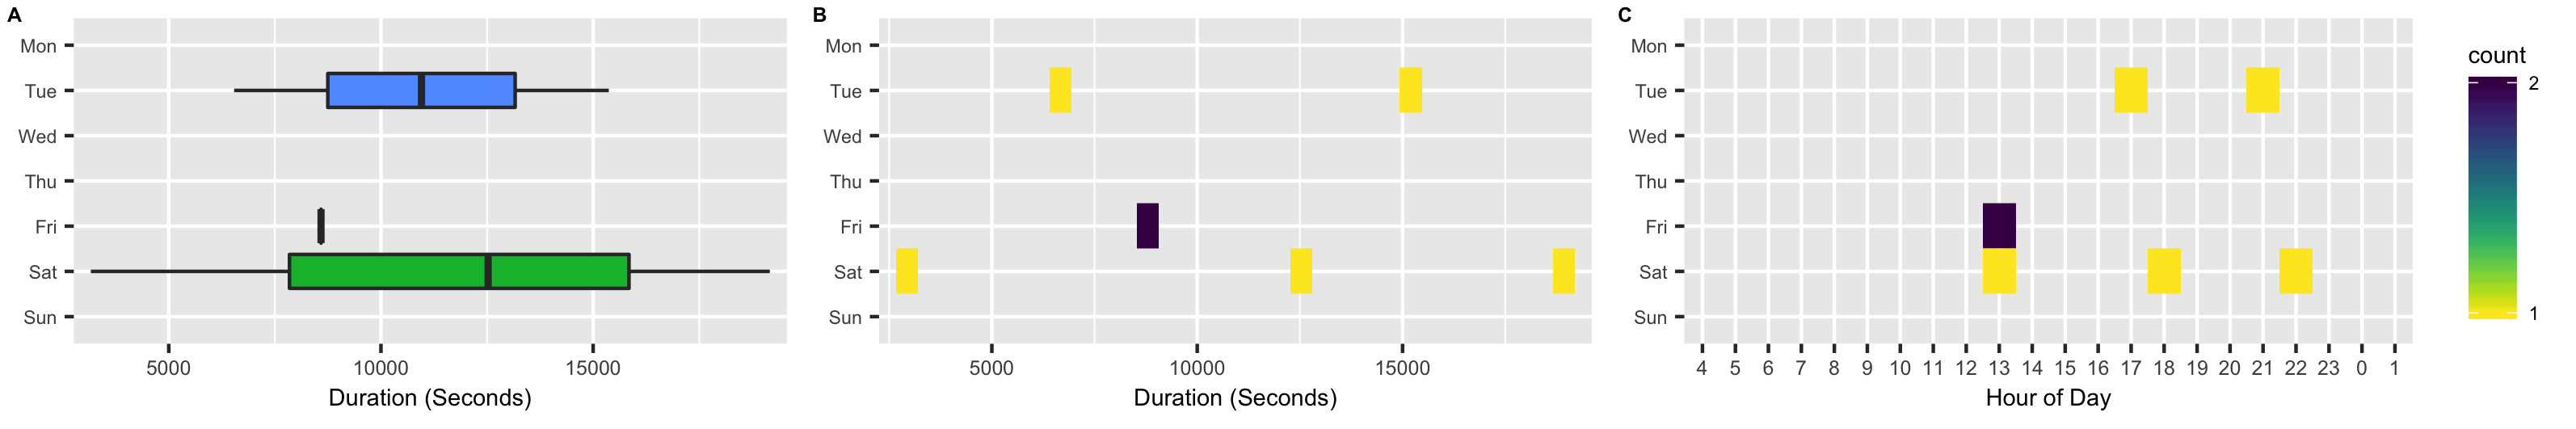
\includegraphics[width=1\linewidth]{/Users/alistairgj/Documents/GitHub/IoT_ResearchProject/IoT_November/images/subAct76} 

}

\caption{Box plot (A) and heat maps (B = day of week versus duration in seconds mapped by count, C = day of week versus hour of day mapped by count) for the Livingroom Lamp sub-activity.}\label{fig:subAct76}
\end{figure}

\hypertarget{kitchen-washingmachine---sub-activity-142}{%
\paragraph{Kitchen Washingmachine - Sub-Activity
142}\label{kitchen-washingmachine---sub-activity-142}}

\begin{figure}[H]

{\centering 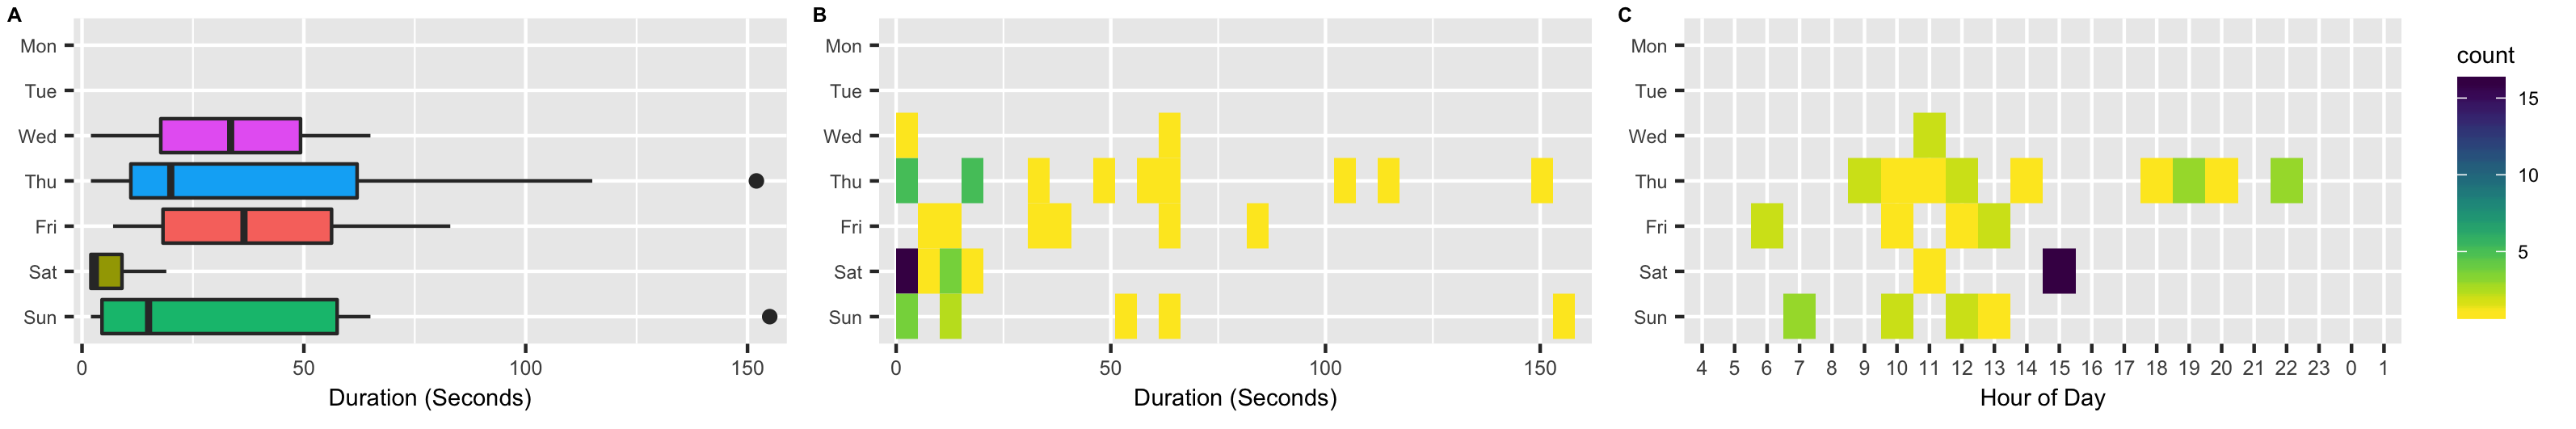
\includegraphics[width=1\linewidth]{/Users/alistairgj/Documents/GitHub/IoT_ResearchProject/IoT_November/images/subAct142} 

}

\caption{Box plot (A) and heat maps (B = day of week versus duration in seconds mapped by count, C = day of week versus hour of day mapped by count) for the Kitchen Washingmachine sub-activity.}\label{fig:subAct142}
\end{figure}

\hypertarget{kitchen-laundry-dryer---sub-activity-90}{%
\paragraph{Kitchen Laundry Dryer - Sub-Activity
90}\label{kitchen-laundry-dryer---sub-activity-90}}

\begin{figure}[H]

{\centering 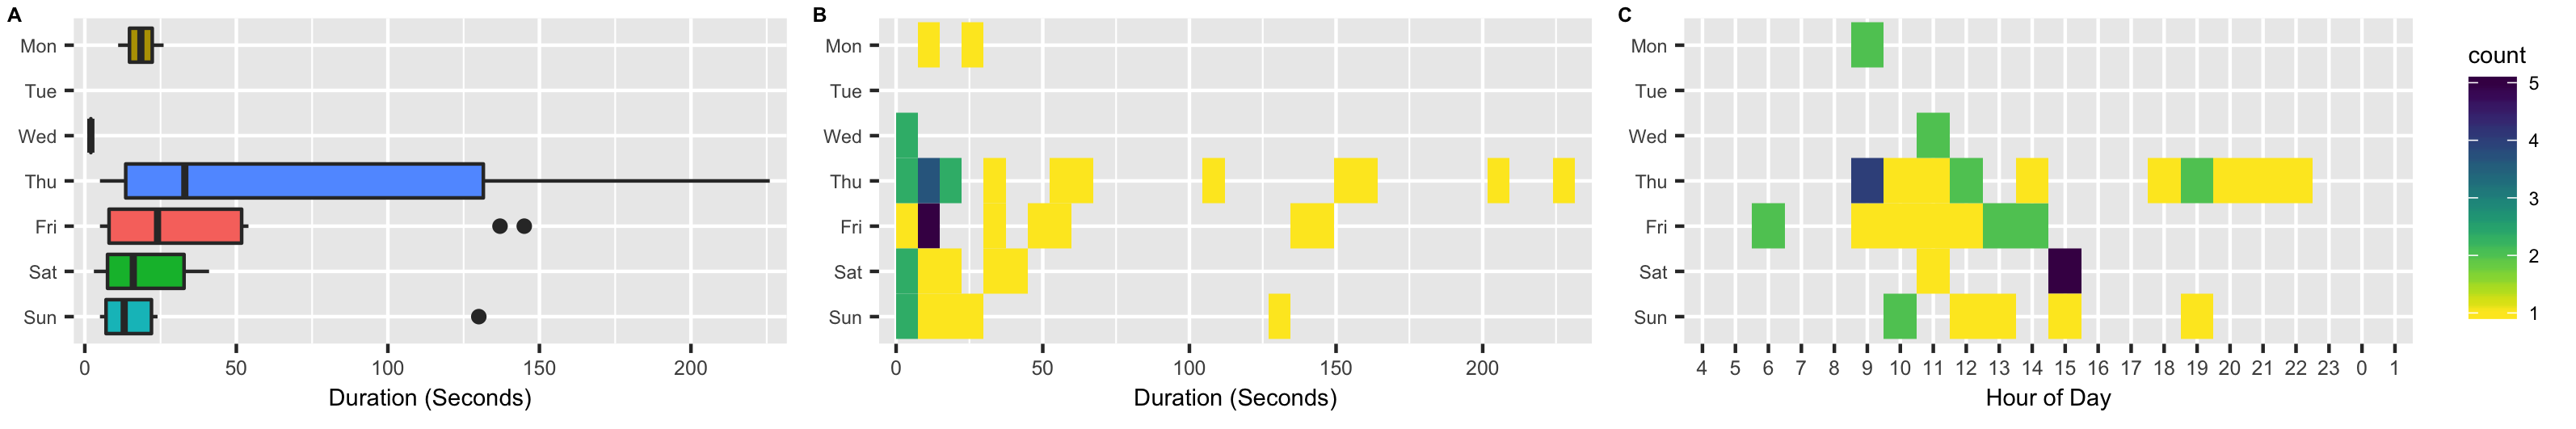
\includegraphics[width=1\linewidth]{/Users/alistairgj/Documents/GitHub/IoT_ResearchProject/IoT_November/images/subAct90} 

}

\caption{Box plot (A) and heat maps (B = day of week versus duration in seconds mapped by count, C = day of week versus hour of day mapped by count) for the Kitchen Laundry Dryer sub-activity.}\label{fig:subAct90}
\end{figure}

\hypertarget{kitchen-garbage-disposal---sub-activity-98}{%
\paragraph{Kitchen Garbage Disposal - Sub-Activity
98}\label{kitchen-garbage-disposal---sub-activity-98}}

\begin{figure}[H]

{\centering 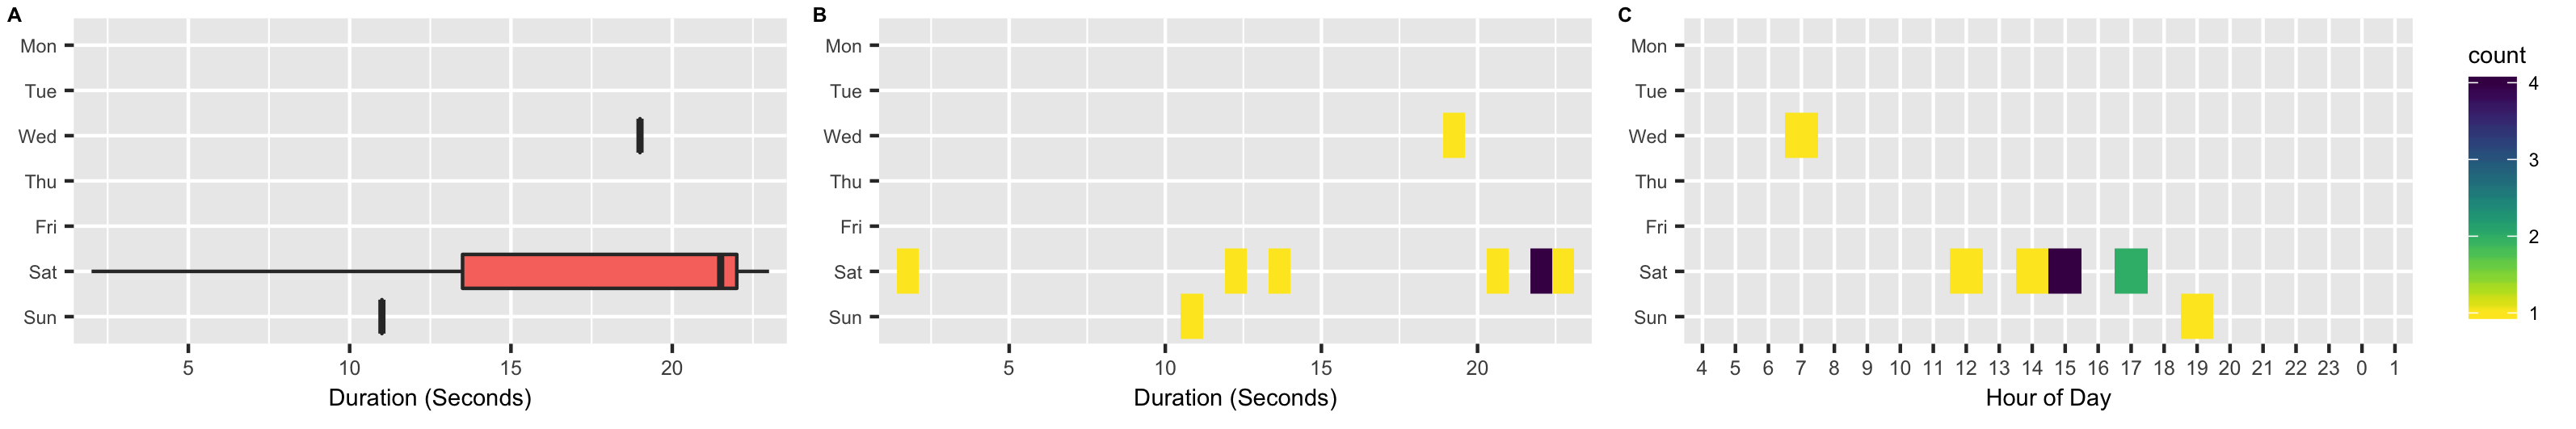
\includegraphics[width=1\linewidth]{/Users/alistairgj/Documents/GitHub/IoT_ResearchProject/IoT_November/images/subAct98} 

}

\caption{Box plot (A) and heat maps (B = day of week versus duration in seconds mapped by count, C = day of week versus hour of day mapped by count) for the Kitchen Garbage Disposal sub-activity.}\label{fig:subAct98}
\end{figure}

\hypertarget{kitchen-coffee-machine---sub-activity-119}{%
\paragraph{Kitchen Coffee Machine - Sub-Activity
119}\label{kitchen-coffee-machine---sub-activity-119}}

\begin{figure}[H]

{\centering 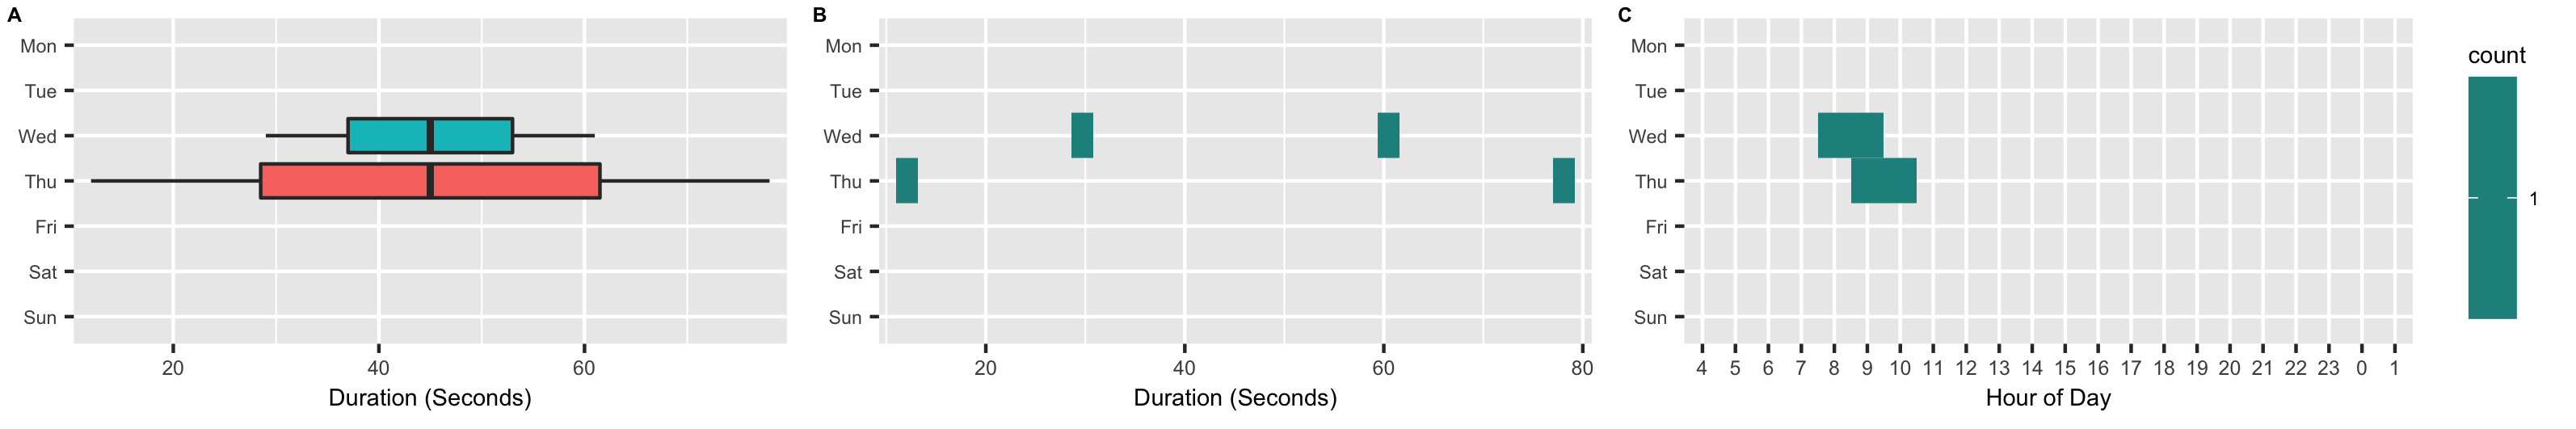
\includegraphics[width=1\linewidth]{/Users/alistairgj/Documents/GitHub/IoT_ResearchProject/IoT_November/images/subAct119} 

}

\caption{Box plot (A) and heat maps (B = day of week versus duration in seconds mapped by count, C = day of week versus hour of day mapped by count) for the Kitchen Coffee Machine sub-activity.}\label{fig:subAct119}
\end{figure}

\hypertarget{subactivity-cleansing---4-sub-activity-dropped}{%
\subsubsection{SubActivity Cleansing - 4) Sub-activity
dropped}\label{subactivity-cleansing---4-sub-activity-dropped}}

Based on the investigation of the box plots (A in all sub activity
plots), heat maps of day of week versus duration in seconds mapped by
count (B in all subactivity plots) and heat maps of day of week versus
hour of day mapped by count (C in all subactivity plots) the following
sub activities were dropped from the dataset. This livingroom DVD sub
activity, as plotted below in Figure \ref{fig:subAct56} was dropped from
the dataset due to it's sparsity (only two instances in the dataset).
Similarly, the bedroom lamp sub-activity, as plotted below in Figure
\ref{fig:subAct64} also had only two instances in the dataset and was
dropped. The bedroom jewelrybox subactivity, as seen in Figure
\ref{fig:subAct139} was dropped due to the extremely specific nature of
this subactivity. In building a generalized model, we do not wish to
have such datapoints present for our analysis. Likewise with the bedroom
jewelry box, the kitchen cereal subactivity, Figure \ref{fig:subAct145}
below, were dropped for the same reason.

\hypertarget{livingroom-dvd---sub-activity-56}{%
\paragraph{Livingroom DVD - Sub-Activity
56}\label{livingroom-dvd---sub-activity-56}}

\begin{figure}[H]

{\centering \includegraphics[width=1\linewidth]{/Users/alistairgj/Documents/GitHub/IoT_ResearchProject/IoT_November/images/subAct56} 

}

\caption{Box plot (A) and heat maps (B = day of week versus duration in seconds mapped by count, C = day of week versus hour of day mapped by count) for the Livingroom DVD sub activity.}\label{fig:subAct56}
\end{figure}

\hypertarget{bedroom-lamp---sub-activity-64}{%
\paragraph{Bedroom Lamp - Sub-Activity
64}\label{bedroom-lamp---sub-activity-64}}

\begin{figure}[H]

{\centering \includegraphics[width=1\linewidth]{/Users/alistairgj/Documents/GitHub/IoT_ResearchProject/IoT_November/images/subAct64} 

}

\caption{Box plot (A) and heat maps (B = day of week versus duration in seconds mapped by count, C = day of week versus hour of day mapped by count) for the Bedroom Lamp sub-activity.}\label{fig:subAct64}
\end{figure}

\hypertarget{bedroom-jewelrybox---sub-activity-139}{%
\paragraph{Bedroom Jewelrybox - Sub-Activity
139}\label{bedroom-jewelrybox---sub-activity-139}}

\begin{figure}[H]

{\centering \includegraphics[width=1\linewidth]{/Users/alistairgj/Documents/GitHub/IoT_ResearchProject/IoT_November/images/subAct139} 

}

\caption{Box plot (A) and heat maps (B = day of week versus duration in seconds mapped by count, C = day of week versus hour of day mapped by count) for the Bedroom Jewelrybox sub activity.}\label{fig:subAct139}
\end{figure}

\hypertarget{kitchen-cereal---sub-activity-145}{%
\paragraph{Kitchen Cereal - Sub-Activity
145}\label{kitchen-cereal---sub-activity-145}}

\begin{figure}[H]

{\centering \includegraphics[width=1\linewidth]{/Users/alistairgj/Documents/GitHub/IoT_ResearchProject/IoT_November/images/subAct145} 

}

\caption{Box plot (A) and heat maps (B = day of week versus duration in seconds mapped by count, C = day of week versus hour of day mapped by count) for the Kitchen Cereal sub-activity.}\label{fig:subAct145}
\end{figure}

\hypertarget{kitchen-containers---sub-activity-60}{%
\paragraph{Kitchen Containers - Sub-Activity
60}\label{kitchen-containers---sub-activity-60}}

\begin{figure}[H]

{\centering \includegraphics[width=1\linewidth]{/Users/alistairgj/Documents/GitHub/IoT_ResearchProject/IoT_November/images/subAct60} 

}

\caption{Box plot (A) and heat maps (B = day of week versus duration in seconds mapped by count, C = day of week versus hour of day mapped by count) for the Kitchen Containers sub-activity.}\label{fig:subAct60}
\end{figure}

\hypertarget{the-final-pre-processed-dataset}{%
\subsubsection{The Final pre-processed
dataset}\label{the-final-pre-processed-dataset}}

The final pre-processed dataset had the following attributes;
\texttt{subActNum} (the aub-activity number from the original
\texttt{S1\ Activities} dataset), \texttt{subAct} (the aub-activity
descriptor from the original \texttt{S1\ Activities} dataset),
\texttt{start} (the start datetime for this specific instance of the
sub-activity), \texttt{end} (the end datetime for this specific instance
of the aub-activity), \texttt{dayNumeric} (a categorical variable to
indiate day), \texttt{DAY} (e.g., `Fri', `Sat'), \texttt{WDWE} (WD
signifies `weekday' and WE signifies `weekend'), \texttt{HOUR} (a
categorical value to indicate time of the day, by the hour).

\hypertarget{data-analysis-and-manipulation}{%
\subsection{Data Analysis and
Manipulation}\label{data-analysis-and-manipulation}}

The primary focus of this section will be qualitative and quantitative
analysis of the pre-processed data. This includes casting the data into
a structure for sequential analysis via Sankey diagrams, and into a
Boolean Array structure for subsequent machine learning.

\hypertarget{sequential-analysis-algorithm}{%
\subsubsection{Sequential Analysis
Algorithm}\label{sequential-analysis-algorithm}}

An algorithm was created to capture the amount of time between the start
of one event (\texttt{Event\ A}) and the start of another event
(\texttt{Event\ B}). In is worth noting that as the target dataset
(Table \ref{tab:}) is row-wise event data on a continuous scale, without
correct bounds, this algorithm would consider the start of every
\texttt{Event\ B} after each \texttt{Event\ A}, subsequently creating an
extremely noisy and large dataset via a combinatorial explosion. In this
scenario, we would have meaningless associations with delta values in
the order of hundreds of thousands of seconds.

The algorithm \texttt{id\_delta} was created to perform sequential
analysis without combinatorial explosion and to capture the amount of
time between the start of \texttt{Event\ A} and the start of event
\texttt{Event\ B}, as the value \texttt{Delta} in seconds. The algorithm
does this by taking three arguments. The first argument,
\texttt{events}, is the dataset with each event occuring as a row
instance. The second argument, \texttt{n}, is the total number of
subsequent \texttt{Event\ B} for any one \texttt{Event\ A}. The final
argument, \texttt{delta\_threshold} takes interger quantities
representative of the number of seconds into the future to consider.

By way of an example \texttt{id\_delta(ds,\ 10,\ dt.timedelta(0,-60))}
for each event row instance in \texttt{ds}, \texttt{10} neighbouring
subevents will be captured, as long as they occur within a range of
\texttt{0} till \texttt{60} seconds forward. In this scenario, if only
four \texttt{Event\ B} occur within sixty seconds of \texttt{EventA}
then only these four will be captured. Likewise, if thirteen
\texttt{EventB} occur within sixty seconds of \texttt{EventA}, then only
ten will be captured.

\begin{Shaded}
\begin{Highlighting}[]
\KeywordTok{def}\NormalTok{ id_delta(events, n}\OperatorTok{=}\DecValTok{1}\NormalTok{, delta_threshold}\OperatorTok{=}\NormalTok{dt.timedelta(}\OperatorTok{-}\DecValTok{99}\NormalTok{)): }\CommentTok{# D}
\NormalTok{    nns }\OperatorTok{=}\NormalTok{ [] }\CommentTok{# Create an empty array}
    \ControlFlowTok{for}\NormalTok{ row }\KeywordTok{in}\NormalTok{ events.itertuples():}
\NormalTok{        start_time }\OperatorTok{=} \BuiltInTok{getattr}\NormalTok{(row, }\StringTok{'start'}\NormalTok{) }\CommentTok{# Extract `start` from data set}
\NormalTok{        end_time }\OperatorTok{=} \BuiltInTok{getattr}\NormalTok{(row, }\StringTok{'end'}\NormalTok{) }\CommentTok{# Extract `end` from data set}
\NormalTok{        subActNum }\OperatorTok{=} \BuiltInTok{getattr}\NormalTok{(row, }\StringTok{'subActNum'}\NormalTok{) }\CommentTok{# Extract `subActNum` from data set}
\NormalTok{        row_index }\OperatorTok{=} \BuiltInTok{getattr}\NormalTok{(row, }\StringTok{'Index'}\NormalTok{) }\CommentTok{# Extract `index` from data set}
        
\NormalTok{        nn }\OperatorTok{=}\NormalTok{ events[(events.start }\OperatorTok{>=}\NormalTok{ start_time) }\OperatorTok{&} \CommentTok{# }
\NormalTok{                    (events.index }\OperatorTok{!=}\NormalTok{ row_index) }\OperatorTok{&} \CommentTok{# }
\NormalTok{                    ((start_time }\OperatorTok{-}\NormalTok{ events.start) }\OperatorTok{>}\NormalTok{ delta_threshold)][:n]}
\NormalTok{        ordered }\OperatorTok{=}\NormalTok{ pd.DataFrame()}
\NormalTok{        ordered[}\StringTok{'Dummy'}\NormalTok{] }\OperatorTok{=}\NormalTok{ nn[}\StringTok{'subActNum'}\NormalTok{] }\CommentTok{# Created for indexing purposes}
\NormalTok{        ordered[}\StringTok{'EventA'}\NormalTok{] }\OperatorTok{=}\NormalTok{ subActNum}
\NormalTok{        ordered[}\StringTok{'EventB'}\NormalTok{] }\OperatorTok{=}\NormalTok{ nn[}\StringTok{'subActNum'}\NormalTok{]}
\NormalTok{        ordered[}\StringTok{'EvA_Start'}\NormalTok{] }\OperatorTok{=}\NormalTok{ start_time}
\NormalTok{        ordered[}\StringTok{'EvB_Start'}\NormalTok{] }\OperatorTok{=}\NormalTok{ nn[}\StringTok{'start'}\NormalTok{]}
\NormalTok{        ordered[}\StringTok{'EvA_End'}\NormalTok{] }\OperatorTok{=}\NormalTok{ end_time}
\NormalTok{        ordered[}\StringTok{'EvB_End'}\NormalTok{] }\OperatorTok{=}\NormalTok{ nn[}\StringTok{'end'}\NormalTok{]}
        \KeywordTok{del}\NormalTok{ ordered[}\StringTok{'Dummy'}\NormalTok{] }\CommentTok{# Dropped}
\NormalTok{        nns.append(ordered)}
  
\NormalTok{    result }\OperatorTok{=}\NormalTok{ pd.concat(nns)}
\NormalTok{    result[}\StringTok{'Delta'}\NormalTok{] }\OperatorTok{=}\NormalTok{ np.where(result[}\StringTok{'EvA_Start'}\NormalTok{] }\OperatorTok{==}\NormalTok{ result[}\StringTok{'EvB_Start'}\NormalTok{], }\DecValTok{0}\NormalTok{,}
\NormalTok{                               (result[}\StringTok{'EvB_Start'}\NormalTok{] }\OperatorTok{-}\NormalTok{ result[}\StringTok{'EvA_Start'}\NormalTok{]))}
\NormalTok{    result[}\StringTok{'Delta'}\NormalTok{] }\OperatorTok{=}\NormalTok{ result[}\StringTok{'Delta'}\NormalTok{].dt.total_seconds()}
    \ControlFlowTok{return}\NormalTok{ result}
\end{Highlighting}
\end{Shaded}

A shotgun analysis of the combinatorics associated with varying input
arguments resulted in the following observations; * One neighbour for 10
seconds gave a dataset of 1063 instances
(\texttt{id\_delta(ds,\ 1,\ dt.timedelta(0,-10))}) * One neighbour for
60 seconds gave a dataset of 1989 instances
(\texttt{id\_delta(ds,\ 1,\ dt.timedelta(0,-60))}) * Ten neighbours for
10 seconds gave a dataset of 1536 instances
(\texttt{id\_delta(ds,\ 10,\ dt.timedelta(0,-10))}) * Ten neighbours for
60 seconds gave a dataset of 5385 instances
(\texttt{id\_delta(ds,\ 10,\ dt.timedelta(0,-60))})

We are focussing our analysis on the sequential analysis algorithm run
with the parameters of one neighbouring sub-activity over a sixty second
period (\texttt{id\_delta(ds,\ 1,\ dt.timedelta(0,-60))}), the head of
the resultant dataset (\texttt{ds\_1n\_60s.csv}) can be Table
\ref{tab:TAB_ds_1n_60s}, below. The reasoning behind chosing this
dataset being 1) It is best practise to start with the most `simple'
form of a problem in order to develop understanding, in this case being
that one neighbour only is considered for each row and 2) For further
analysis these data may be collapsed from a seconds time scale to a
minute time scale, so it is useful to know the variety of activities
that can occur within one minute (60 seconds of each other).

\rowcolors{2}{gray!6}{white}
\begin{table}[!h]

\caption{\label{tab:TAB_ds_1n_60s}Sequential analysis result: one neighbouring sub-activity over a sixty second period}
\centering
\resizebox{\linewidth}{!}{\fontsize{8}{10}\selectfont
\begin{tabular}[t]{rrllllrllr}
\hiderowcolors
\toprule
EventA & EventB & EvA\_Start & EvB\_Start & EvA\_End & EvB\_End & Delta & DAY & WDWE & Hour\\
\midrule
\showrowcolors
67 & 100 & 2003-03-27 06:43:40 & 2003-03-27 06:44:06 & 2003-03-27 06:43:44 & 2003-03-27 06:44:07 & 26 & Thu & WD & 6\\
100 & 101 & 2003-03-27 06:44:06 & 2003-03-27 06:44:20 & 2003-03-27 06:44:07 & 2003-03-27 07:46:35 & 14 & Thu & WD & 6\\
101 & 57 & 2003-03-27 06:44:20 & 2003-03-27 06:44:35 & 2003-03-27 07:46:35 & 2003-03-27 06:44:49 & 15 & Thu & WD & 6\\
57 & 57 & 2003-03-27 06:44:35 & 2003-03-27 06:44:36 & 2003-03-27 06:44:49 & 2003-03-27 06:44:49 & 1 & Thu & WD & 6\\
57 & 67 & 2003-03-27 06:44:36 & 2003-03-27 06:44:49 & 2003-03-27 06:44:49 & 2003-03-27 06:44:57 & 13 & Thu & WD & 6\\
\addlinespace
67 & 82 & 2003-03-27 06:44:49 & 2003-03-27 06:45:45 & 2003-03-27 06:44:57 & 2003-03-27 06:45:49 & 56 & Thu & WD & 6\\
\bottomrule
\end{tabular}}
\end{table}
\rowcolors{2}{white}{white}

\hypertarget{qualitative-sequential-analysis-via-sankey-diagram}{%
\subsubsection{Qualitative Sequential Analysis via Sankey
Diagram}\label{qualitative-sequential-analysis-via-sankey-diagram}}

In order to develop understanding of the interrelaterness of the
sub-activites, the data from the sequential analysis
\texttt{ds\_1n\_60s.csv} were plotted as Sankey diagrams using a bespoke
wrapper method written in Python. Using the previously mentioned
features of \texttt{HOUR} and \texttt{WDWE} in the dataset, the
resultant diagrams were segmented over 6 time periods, namely:

\begin{enumerate}
\def\labelenumi{\arabic{enumi}.}
\tightlist
\item
  Figure \ref{fig:sankey_WeekdayMorningds_1n_60s} - Weekday Morning,
  initial morning sub-activity until 11.59 am
\item
  Figure \ref{fig:sankey_WeekdayAfternoonds_1n_60s} - Weekday Afternoon,
  12 noon until 17.59 pm
\item
  Figure \ref{fig:sankey_WeekdayEveningds_1n_60s} - Weekday Evening,
  18:00 pm until mid-night
\item
  Figure \ref{fig:sankey_WeekendMorningds_1n_60s} - Weekend Morning,
  initial morning sub-activity until 11.59 am
\item
  Figure \ref{fig:sankey_WeekendAfternoonds_1n_60s} - Weekend Afternoon,
  12 noon until 17.59pm
\item
  Figure \ref{fig:sankey_WeekendEveningds_1n_60s} - Weekend Evening,
  18:00pm untill mid-night
\end{enumerate}

Sankey diagrams are used to visualise flows of energy, materials or
other resources in a variety of applications (Lupton, 2017).In our case,
the Sankey diagrams will allow us to visualise the flow of end-user
interaction with each sub-activity over the time-boxes 1 through 6, as
described above. Our Sankey diagrams (derived from the 1 neighbour over
60 seconds sequential analysis) have the following features i) The each
represent a specific aggregated time period from the dataset, ii) In
each Sankey, the sub-acitivity nodes that require energy input only from
the end user (e.g., Kitchen Door) are blue, while the sub-activity nodes
that require external energy to function (e.g., Kitchen Toaster), iii)
The width of each sub-activity in the Sankey diagram is indicative to
the number of times interaction occured, a thicker node means more
interaction, iv) The lines between each node indicate the event of one
sub-activity proceeding or preceeding another and v) Some events nodes
are centralised, with at least one activity `flowing in' and at least
one `flowing out' while other nodes a terminal, with only activities
`flowing in' or `flowing out' (but not both).

Each Sankey diagram, as seen below, shows a high level of interactivity
between the various sub-acitivities. We observer that of all the `no
external energy' sub-activities, only the foyer closet (as seen in
Figure \ref{fig:sankey_WeekdayAfternoonds_1n_60s} and Figure
\ref{fig:sankey_WeekdayEveningds_1n_60s}) acts as a terminal node. In
comparision, numerous sub-activities that require energy (as seen in
Figure \ref{fig:sankey_WeekdayEveningds_1n_60s} and Figure
\ref{fig:sankey_WeekendEveningds_1n_60s}) act as terminal nodes. We also
observe that there is a very level of interactivity between the
sub-activities that do and do no require an external energy source (red
and blue nodes, respectively) to function. This will provide direction
for further analyis.

\hypertarget{weekday-morning-initial-morning-sub-activity-until-11.59-am}{%
\paragraph{Weekday Morning, initial morning sub-activity until 11.59
am}\label{weekday-morning-initial-morning-sub-activity-until-11.59-am}}

\begin{figure}[H]

{\centering \includegraphics[width=1\linewidth]{/Users/alistairgj/Documents/GitHub/IoT_ResearchProject/IoT_November/images/WeekdayMorningds_1n_60s} 

}

\caption{Sankey Diagram of Weekday Mornings, considering all one neighbour per instance within a 60 second period}\label{fig:sankey_WeekdayMorningds_1n_60s}
\end{figure}

\pagebreak

\hypertarget{weekday-afternoon-12-noon-until-17.59-pm}{%
\paragraph{Weekday Afternoon, 12 noon until 17.59
pm}\label{weekday-afternoon-12-noon-until-17.59-pm}}

\begin{figure}[H]

{\centering \includegraphics[width=1\linewidth]{/Users/alistairgj/Documents/GitHub/IoT_ResearchProject/IoT_November/images/WeekdayAfternoonds_1n_60s} 

}

\caption{Sankey Diagram of Weekday Afternoons, considering all one neighbour per instance within a 60 second period}\label{fig:sankey_WeekdayAfternoonds_1n_60s}
\end{figure}

\hypertarget{weekday-evening-1800-pm-until-mid-night}{%
\paragraph{Weekday Evening, 18:00 pm until
mid-night}\label{weekday-evening-1800-pm-until-mid-night}}

\begin{figure}[H]

{\centering \includegraphics[width=1\linewidth]{/Users/alistairgj/Documents/GitHub/IoT_ResearchProject/IoT_November/images/WeekdayEveningds_1n_60s} 

}

\caption{Sankey Diagram of Weekday Evenings, considering all one neighbour per instance within a 60 second period}\label{fig:sankey_WeekdayEveningds_1n_60s}
\end{figure}

\pagebreak

\hypertarget{weekend-morning-initial-morning-sub-activity-until-11.59-am}{%
\paragraph{Weekend Morning, initial morning sub-activity until 11.59
am}\label{weekend-morning-initial-morning-sub-activity-until-11.59-am}}

\begin{figure}[H]

{\centering \includegraphics[width=1\linewidth]{/Users/alistairgj/Documents/GitHub/IoT_ResearchProject/IoT_November/images/WeekendMorningds_1n_60s} 

}

\caption{Sankey Diagram of Weekend Mornings, considering all one neighbour per instance within a 60 second period}\label{fig:sankey_WeekendMorningds_1n_60s}
\end{figure}

\hypertarget{weekend-afternoon-12-noon-until-17.59pm}{%
\paragraph{Weekend Afternoon, 12 noon until
17.59pm}\label{weekend-afternoon-12-noon-until-17.59pm}}

\begin{figure}[H]

{\centering \includegraphics[width=1\linewidth]{/Users/alistairgj/Documents/GitHub/IoT_ResearchProject/IoT_November/images/WeekendAfternoonds_1n_60s} 

}

\caption{Sankey Diagram of Weekend Afternoons, considering all one neighbour per instance within a 60 second period}\label{fig:sankey_WeekendAfternoonds_1n_60s}
\end{figure}

\pagebreak

\hypertarget{weekend-evening-1800pm-untill-mid-night}{%
\paragraph{Weekend Evening, 18:00pm untill
mid-night}\label{weekend-evening-1800pm-untill-mid-night}}

\begin{figure}[H]

{\centering \includegraphics[width=1\linewidth]{/Users/alistairgj/Documents/GitHub/IoT_ResearchProject/IoT_November/images/WeekendEveningds_1n_60s} 

}

\caption{Sankey Diagram of Weekend Evenings, considering all one neighbour per instance within a 60 second period}\label{fig:sankey_WeekendEveningds_1n_60s}
\end{figure}

\hypertarget{re-casting-the-dataset-as-a-boolean-array}{%
\subsubsection{Re-casting the Dataset as a Boolean
Array}\label{re-casting-the-dataset-as-a-boolean-array}}

Based on the analysis above, we sought a data structure whereby every
simultaneous subactivity occuring at one point in time could potentially
be evaluated. In order to acheive this without having to place a large
emphasis on complex combinatorics, it was decided to cast the data
structure into a Boolean Array. In this structure, each sub-activity
will become an attribute, with every row is a timestamp index. This
structure will span the duration of the dataset - in other words, every
second that was accounted for in the original dataset will have a row
instance (a row).

The required transformations were for performed on the pre-processed
dataset, with an initial index occuring at 27/03/2003 6:43:40 am, and
the final index occuring at 11/4/2003 10:24:18 pm. In some regions of
the dataset there were no results, so it is not an uninterrupted
timescale from the first to last index. This will not affect our
analysis as we are considering sequences of events as they occur with
respect to concurrency.

A sample of the processed boolean array data (with omitted attributes)
can be seen below in Table \ref{tab:TAB_S1SubAct_B_s_EXAMPLE}. Here we
can see the following sub-activities in an `active' state; 57 (bathroom
medicine cabinet), 101 (bathroom lightswitch) and 96 (bathroom
exhaustfan). All other sub-activities are inactive. At 01/04/2003
6:54:56 am sub-activity 88 (bathroom sinkfaucet - hot) becomes active,
followed by one second later at 01/04/2003 6:54:57 am sub-activity 68
(bathroom sinkfaucet - cold) becoming active. Sub-activity 57, 101, 68,
88 and 96 all remain active at 01/04/2003 6:55:01 am.

\rowcolors{2}{gray!6}{white}
\begin{table}[!h]

\caption{\label{tab:TAB_S1SubAct_B_s_EXAMPLE}Add text}
\centering
\fontsize{8}{10}\selectfont
\begin{tabular}[t]{lrrrrrrrrrrr}
\hiderowcolors
\toprule
IDX & 57 & 67 & 100 & 101 & 104 & 68 & 93 & 88 & 90 & 96 & 130\\
\midrule
\showrowcolors
01/04/2003  6:54:50 am & 1 & 0 & 0 & 1 & 0 & 0 & 0 & 0 & 0 & 1 & 0\\
01/04/2003  6:54:51 am & 1 & 0 & 0 & 1 & 0 & 0 & 0 & 0 & 0 & 1 & 0\\
01/04/2003  6:54:52 am & 1 & 0 & 0 & 1 & 0 & 0 & 0 & 0 & 0 & 1 & 0\\
01/04/2003  6:54:53 am & 1 & 0 & 0 & 1 & 0 & 0 & 0 & 0 & 0 & 1 & 0\\
01/04/2003  6:54:54 am & 1 & 0 & 0 & 1 & 0 & 0 & 0 & 0 & 0 & 1 & 0\\
\addlinespace
01/04/2003  6:54:55 am & 1 & 0 & 0 & 1 & 0 & 0 & 0 & 0 & 0 & 1 & 0\\
01/04/2003  6:54:56 am & 1 & 0 & 0 & 1 & 0 & 0 & 0 & 1 & 0 & 1 & 0\\
01/04/2003  6:54:57 am & 1 & 0 & 0 & 1 & 0 & 1 & 0 & 1 & 0 & 1 & 0\\
01/04/2003  6:54:58 am & 1 & 0 & 0 & 1 & 0 & 1 & 0 & 1 & 0 & 1 & 0\\
01/04/2003  6:54:59 am & 1 & 0 & 0 & 1 & 0 & 1 & 0 & 1 & 0 & 1 & 0\\
\addlinespace
01/04/2003  6:55:00 am & 1 & 0 & 0 & 1 & 0 & 1 & 0 & 1 & 0 & 1 & 0\\
01/04/2003  6:55:01 am & 1 & 0 & 0 & 1 & 0 & 1 & 0 & 1 & 0 & 1 & 0\\
\bottomrule
\end{tabular}
\end{table}
\rowcolors{2}{white}{white}

This data structure thus offers the following benefits; i) Simultaneous
consideration of the state of multiple sub-activities,ii) Present in a
format that is still readily human interprettable and iii) Present in a
format that can be easily consumed by a machine.

And the following challenges; i) The dataset is overall very large,
potentially requiring large amounts of computational power for
downstream analysis, ii) The dataset is potentially highly homogeneous
in certain temporal regions and iii) A second-by-second analysis is most
likely to granular for the purposes of this work

In order to remedy this, we converted the Boolean Array structure into
the minute-scale, by aggregating all the second values for each
attribute for each minute. For example, if a sub-activity had occured
for 30 seconds during one minute, it will not be represented as a `1'
for that minute in the dataframe.

\rowcolors{2}{gray!6}{white}
\begin{table}[!h]

\caption{\label{tab:TAB_S1SubAct_B_m_EXAMPLE}Add text}
\centering
\fontsize{8}{10}\selectfont
\begin{tabular}[t]{lrrrrrrrrrrr}
\hiderowcolors
\toprule
IDX & 57 & 67 & 100 & 101 & 104 & 68 & 93 & 88 & 90 & 96 & 130\\
\midrule
\showrowcolors
01/04/2003  6:45:00 am & 1 & 0 & 0 & 1 & 0 & 0 & 0 & 0 & 0 & 1 & 0\\
01/04/2003  6:46:00 am & 1 & 0 & 0 & 1 & 0 & 0 & 0 & 0 & 0 & 1 & 0\\
01/04/2003  6:47:00 am & 1 & 0 & 0 & 1 & 0 & 0 & 0 & 0 & 0 & 1 & 0\\
01/04/2003  6:48:00 am & 1 & 0 & 0 & 1 & 0 & 0 & 0 & 0 & 0 & 1 & 0\\
01/04/2003  6:49:00 am & 1 & 0 & 0 & 1 & 0 & 0 & 0 & 0 & 0 & 1 & 0\\
\addlinespace
01/04/2003  6:51:00 am & 1 & 0 & 0 & 1 & 0 & 0 & 0 & 0 & 0 & 1 & 0\\
01/04/2003  6:52:00 am & 1 & 0 & 0 & 1 & 0 & 0 & 0 & 0 & 0 & 1 & 0\\
01/04/2003  6:53:00 am & 1 & 0 & 0 & 1 & 0 & 0 & 0 & 0 & 0 & 1 & 0\\
01/04/2003  6:54:00 am & 1 & 0 & 0 & 1 & 0 & 1 & 0 & 0 & 0 & 1 & 0\\
01/04/2003  6:55:00 am & 1 & 0 & 0 & 1 & 0 & 1 & 0 & 1 & 0 & 1 & 0\\
\addlinespace
01/04/2003  6:56:00 am & 1 & 0 & 0 & 1 & 0 & 1 & 0 & 1 & 0 & 1 & 0\\
01/04/2003  6:57:00 am & 1 & 0 & 0 & 1 & 0 & 0 & 0 & 0 & 0 & 1 & 0\\
\bottomrule
\end{tabular}
\end{table}
\rowcolors{2}{white}{white}

\hypertarget{machine-learning-analysis}{%
\section{Machine Learning Analysis}\label{machine-learning-analysis}}

Using the pre-processed boolean array data (minute-scale) we will now
attempt to create a predictive model with the aim of identifying
patterns of co-occurrence between the sub-activities. As we are
attempting to predict the on or off state of activities, this is a
binary classification problem. As discussed during the Sankey analysis,
the sub-activities can be broadly categorised as requiring energy input
only from the end user (e.g., Kitchen Door) or requiring external energy
to function (e.g., Kitchen Toaster). Note that for the purposes of
further discussion such appliances will be referred to as
energy-intensive (e.g., light switch, fridge and so on). Our model we
will only attempt to predict the state of energy-intensive appliances,
for reasons outlined in the discussion section.

\hypertarget{the-machine-learning-algorithm}{%
\subsection{The Machine Learning
Algorithm}\label{the-machine-learning-algorithm}}

A wrapper method will be created centered around the the sklearn
Decision Tree Classifier. This method will use a decision tree model and
optimize its hyperparameters using a grid search. The grid search will
be performed over split criterion (`gini' and `entropy') and maximum
depth. Feature selection will be performed using the entropy-based
method of mutual information, for the top five features.
Cross-validation will be performed using 5-folds. The wrapper method
will enable the model to perform the functions described above in an
iterative fashion for each of the energy-intensive sub-activity features
in the dataset. The processed sub-activities meta data will also be
parsed to provide the data on which sub-activity is energy intensive and
which is not. Throughout the iterations, key data will be parsed to
*.csv format for later analysis.

\hypertarget{data}{%
\subsubsection{Data}\label{data}}

The dataset used will be the boolean array on the minute scale. In
preparation for the analysis, the datetime index is removed, as will be
discussed below. Important to note that these data currently contain no
categorical features (e.g, day of week, weekend / weekday, hour of day,
room of house, e.t.c,).

\hypertarget{the-wrapper-method}{%
\subsubsection{The Wrapper Method}\label{the-wrapper-method}}

The following python script was used to perform the desired machine
learning analysis.

\begin{Shaded}
\begin{Highlighting}[]
\ControlFlowTok{for}\NormalTok{ subAct }\KeywordTok{in}\NormalTok{ poweredSubActs:}
\NormalTok{    row }\OperatorTok{=}\NormalTok{ \{}\StringTok{"Target"}\NormalTok{:subAct\}}
\NormalTok{    Data }\OperatorTok{=}\NormalTok{ ds.drop(columns }\OperatorTok{=}\NormalTok{ subAct).values}
\NormalTok{    target }\OperatorTok{=}\NormalTok{ ds[subAct]}
\NormalTok{    D_train, D_test, t_train, t_test }\OperatorTok{=}\NormalTok{ train_test_split(Data, target, test_size }\OperatorTok{=} \FloatTok{0.3}\NormalTok{, }
\NormalTok{                                        random_state}\OperatorTok{=}\DecValTok{999}\NormalTok{)}
\NormalTok{    cv_method }\OperatorTok{=}\NormalTok{ RepeatedStratifiedKFold(n_splits }\OperatorTok{=} \DecValTok{5}\NormalTok{, n_repeats }\OperatorTok{=} \DecValTok{3}\NormalTok{, random_state }\OperatorTok{=} \DecValTok{999}\NormalTok{)}
\NormalTok{    dt_classifier }\OperatorTok{=}\NormalTok{ DecisionTreeClassifier(random_state}\OperatorTok{=}\DecValTok{999}\NormalTok{)}
\NormalTok{    params_DT }\OperatorTok{=}\NormalTok{ \{}\StringTok{'criterion'}\NormalTok{: [}\StringTok{'gini'}\NormalTok{, }\StringTok{'entropy'}\NormalTok{], }
                \StringTok{'max_depth'}\NormalTok{: [}\DecValTok{2}\NormalTok{, }\DecValTok{3}\NormalTok{, }\DecValTok{4}\NormalTok{, }\DecValTok{5}\NormalTok{, }\DecValTok{6}\NormalTok{, }\DecValTok{7}\NormalTok{, }\DecValTok{8}\NormalTok{, }\DecValTok{9}\NormalTok{, }\DecValTok{10}\NormalTok{]\}}
\NormalTok{    gs }\OperatorTok{=}\NormalTok{ GridSearchCV(estimator}\OperatorTok{=}\NormalTok{dt_classifier, param_grid}\OperatorTok{=}\NormalTok{params_DT, cv}\OperatorTok{=}\NormalTok{cv_method,}
\NormalTok{                      verbose}\OperatorTok{=}\DecValTok{1}\NormalTok{, scoring}\OperatorTok{=}\StringTok{'accuracy'}\NormalTok{)}
\NormalTok{    gs.fit(Data, target)}
\NormalTok{    row[}\StringTok{'Original_Fit'}\NormalTok{] }\OperatorTok{=}\NormalTok{ gs.best_score_}
\NormalTok{    num_features }\OperatorTok{=} \DecValTok{5}
    
\NormalTok{    fs_fit_mutual_info }\OperatorTok{=}\NormalTok{ fs.SelectKBest(fs.mutual_info_classif, k}\OperatorTok{=}\NormalTok{num_features)}
\NormalTok{    fs_fit_mutual_info.fit_transform(Data, target)}
\NormalTok{    fs_indices_mutual_info }\OperatorTok{=}\NormalTok{ np.argsort(fs_fit_mutual_info.scores_)[::}\OperatorTok{-}\DecValTok{1}\NormalTok{][}\DecValTok{0}\NormalTok{:num_features]}
\NormalTok{    best_features_mutual_info }\OperatorTok{=}\NormalTok{ ds.columns[fs_indices_mutual_info].values    }
\NormalTok{    feature_importances_mutual_info }\OperatorTok{=}\NormalTok{ fs_fit_mutual_info.scores_[fs_indices_mutual_info]}
\NormalTok{    results_DT }\OperatorTok{=}\NormalTok{ pd.DataFrame(gs.cv_results_[}\StringTok{'params'}\NormalTok{])}
\NormalTok{    results_DT[}\StringTok{'test_score'}\NormalTok{] }\OperatorTok{=}\NormalTok{ gs.cv_results_[}\StringTok{'mean_test_score'}\NormalTok{]}
\NormalTok{    results_DT.to_csv(subAct }\OperatorTok{+} \StringTok{"_dt.csv"}\NormalTok{, index}\OperatorTok{=}\VariableTok{False}\NormalTok{)}
    
\NormalTok{    t_pred }\OperatorTok{=}\NormalTok{ gs.predict(D_test)}
\NormalTok{    t_prob }\OperatorTok{=}\NormalTok{ gs.predict_proba(D_test)}
\NormalTok{    metrics.roc_auc_score(t_test, t_pred)}
\NormalTok{    fpr, tpr, _ }\OperatorTok{=}\NormalTok{ metrics.roc_curve(t_test, t_prob[:, }\DecValTok{1}\NormalTok{])}
\NormalTok{    roc_auc }\OperatorTok{=}\NormalTok{ metrics.auc(fpr, tpr)    }
\NormalTok{    df }\OperatorTok{=}\NormalTok{ pd.DataFrame(\{}\StringTok{'fpr'}\NormalTok{: fpr, }\StringTok{'tpr'}\NormalTok{: tpr\})}
\NormalTok{    df.to_csv(subAct }\OperatorTok{+} \StringTok{"_roc.csv"}\NormalTok{, index }\OperatorTok{=} \VariableTok{False}\NormalTok{)}
    
\NormalTok{    report }\OperatorTok{=}\NormalTok{ metrics.classification_report(t_test, t_pred, output_dict}\OperatorTok{=}\VariableTok{True}\NormalTok{)}
\NormalTok{    rep }\OperatorTok{=}\NormalTok{ pd.DataFrame(report).transpose()}
\NormalTok{    rep.to_csv(subAct }\OperatorTok{+} \StringTok{"_rep.csv"}\NormalTok{, index}\OperatorTok{=}\VariableTok{True}\NormalTok{)}
    
\NormalTok{    report }\OperatorTok{=}\NormalTok{ metrics.confusion_matrix(t_test, t_pred)}
\NormalTok{    rep }\OperatorTok{=}\NormalTok{ pd.DataFrame(report).transpose()}
\NormalTok{    rep.to_csv(subAct }\OperatorTok{+} \StringTok{"_confusion.csv"}\NormalTok{, index}\OperatorTok{=}\VariableTok{True}\NormalTok{)    }
\end{Highlighting}
\end{Shaded}

\hypertarget{machine-learning-model-results}{%
\subsubsection{Machine Learning Model
Results}\label{machine-learning-model-results}}

The following section provides an evaluation of the machine learning
model results.

\hypertarget{bedroom-lightswitch---sub-activity-108-1}{%
\paragraph{Bedroom Lightswitch - Sub-Activity
108}\label{bedroom-lightswitch---sub-activity-108-1}}

The top five most important features for predicting this sub-activity
(as shown in tile `A' of the plot below) are: bathroom light switch,
kitchen cabinet, kitchen dishwasher, kitchen laundry dryer and
livingroom light switch. The bathroom light switch is significantly more
important than the other four. For the analysis of the bedroom light
switch feature it was determined that the best parameters were `entropy'
with a maximum tree depth of 4. The plot of Mean CV Score versus Maximum
depth shows that `gini' is the better parameter at certain tree depths.
The shape of the ROC curve and the corresponding ROC\_AUC value of
0.9016 are indicative of a good fit. The extremely high precision (0.98)
and recall (1.00) values for 0 as compared to the relatively low recall
(0.36) value for 1 are due to the unbalanced data set, where of the 1588
instances, 1543 are 0, while 45 are 1.

\begin{figure}[H]

{\centering \includegraphics[width=1\linewidth]{/Users/alistairgj/Documents/GitHub/IoT_ResearchProject/IoT_November/images/bedroom_lightswitch_allFeatures} 

}

\caption{Plot of Mutual Information Feature Importance (A), DT Performance Comparison (B) and ROC Curve of DT (C)}\label{fig:unnamed-chunk-7}
\end{figure}

\hypertarget{kitchen-laundry-dryer---sub-activity-90-1}{%
\paragraph{Kitchen Laundry Dryer - Sub-Activity
90}\label{kitchen-laundry-dryer---sub-activity-90-1}}

The top five most important features for predicting this sub-activity
(as shown in tile `A' of the plot below) are: kitchen door, kitchen
washing machine, bathroom medicine cabinet, kitchen dishwasher and
bedroom drawer. The kitchen door and kitchen washing machine are
significantly more important than the other three. For the analysis of
the kitchen laundry dryer feature it was determined that the best
parameter¬s were `gini' with a maximum tree depth of 5. The plot of Mean
CV Score versus Maximum depth shows that `gini' is the better parameter
at all tree depths up to 10. The shape of the ROC curve and the
corresponding ROC\_AUC value of 0.9551 are indicative of a good fit. The
extremely high precision (0.99) and recall (1.00) values for 0 as
compared to the relatively low recall (0.30) value for 1 are due to the
unbalanced data set, where of the 1588 instances, 1565 are 0, while 23
are 1.

\begin{figure}[H]

{\centering \includegraphics[width=1\linewidth]{/Users/alistairgj/Documents/GitHub/IoT_ResearchProject/IoT_November/images/kitchen_laundrydryer_allFeatures} 

}

\caption{Plot of Mutual Information Feature Importance (A), DT Performance Comparison (B) and ROC Curve of DT (C)}\label{fig:unnamed-chunk-8}
\end{figure}

\hypertarget{kitchen-freezer---sub-activity-137-1}{%
\paragraph{Kitchen Freezer - Sub-Activity
137}\label{kitchen-freezer---sub-activity-137-1}}

The top five most important features for predicting this sub-activity
(as shown in tile `A' of the plot below) are: kitchen refrigerator,
livingroom light switch, foyer closet, bathroom door and bathroom toilet
flush. The kitchen refrigerator is significantly more important than the
other four. For the analysis of the kitchen freezer feature it was
determined that the best parameters were `gini' with a maximum tree
depth of 9. The plot of Mean CV Score versus Maximum depth shows that
`gini' is the better parameter at all tree depths from 3 up to 10. The
shape of the ROC curve and the corresponding ROC\_AUC value of 0.8639
are indicative of a good fit. The extremely high precision (0.94) and
recall (0.98) values for 0 as compared to the relatively low recall
(0.44) value for 1 are due to the unbalanced data set, where of the 1588
instances, 1423 are 0, while 165 are 1. The model has successfully
categorised 73 of the 165 instances of 1, and in these circumstances has
performed adequately.

\begin{figure}[H]

{\centering \includegraphics[width=1\linewidth]{/Users/alistairgj/Documents/GitHub/IoT_ResearchProject/IoT_November/images/kitchen_freezer_allFeatures} 

}

\caption{Plot of Mutual Information Feature Importance (A), DT Performance Comparison (B) and ROC Curve of DT (C)}\label{fig:unnamed-chunk-9}
\end{figure}

\hypertarget{kitchen-toaster---sub-activity-131-1}{%
\paragraph{Kitchen Toaster - Sub-Activity
131}\label{kitchen-toaster---sub-activity-131-1}}

The top five most important features for predicting this sub-activity
(as shown in tile `A' of the plot below) are: kitchen cabinet, bathroom
exhaust fan, study light switch, kitchen toaster and livingroom light
switch. The kitchen cabinet is significantly more important than the
other four. For the analysis of the kitchen toaster feature it was
determined that the best parameters were `gini' with a maximum tree
depth of 3. The plot of Mean CV Score versus Maximum depth shows that
`gini' is the better parameter at all tree depths up to 6, and then
`entropy' is the better parameter from 7 to 10. The shape of the ROC
curve and the corresponding ROC\_AUC value of 0.7782 are indicative of
an adequate fit. The extremely high precision (0.99) and recall (1.00)
values for 0 as compared to the relatively low recall (0.23) value for 1
are due to the unbalanced data set, where of the 1588 instances, 1566
are 0, while 22 are 1.

\begin{figure}[H]

{\centering \includegraphics[width=1\linewidth]{/Users/alistairgj/Documents/GitHub/IoT_ResearchProject/IoT_November/images/kitchen_toaster_allFeatures} 

}

\caption{Plot of Mutual Information Feature Importance (A), DT Performance Comparison (B) and ROC Curve of DT (C)}\label{fig:unnamed-chunk-10}
\end{figure}

\hypertarget{bathroom-exhaust-fan---sub-activity-96-1}{%
\paragraph{Bathroom Exhaust Fan - Sub-Activity
96}\label{bathroom-exhaust-fan---sub-activity-96-1}}

The top five most important features for predicting this sub-activity
(as shown in tile `A' of the plot below) are: livingroom light switch,
bathroom sink faucet hot, livingroom lamp, bathroom medicine cabinet and
foyer door. The livingroom light switch, bathroom sink faucet hot and
livingroom lamp are noticeably more important than the other two. For
the analysis of the bathroom exhaust fan feature it was determined that
the best parameters were `gini' with a maximum tree depth of 8. The plot
of Mean CV Score versus Maximum depth shows that `gini' is the better
parameter at all tree depths up to 10. The shape of the ROC curve and
the corresponding ROC\_AUC value of 0.9054 are indicative of a good fit.
The extremely high precision (0.90) and recall (0.99) values for 0 as
compared to the relatively low recall (0.25) value for 1 are due to the
unbalanced data set, where of the 1588 instances, 1384 are 0, while 204
are 1.

\begin{figure}[H]

{\centering \includegraphics[width=1\linewidth]{/Users/alistairgj/Documents/GitHub/IoT_ResearchProject/IoT_November/images/bathroom_exhaustfan_allFeatures} 

}

\caption{Plot of Mutual Information Feature Importance (A), DT Performance Comparison (B) and ROC Curve of DT (C)}\label{fig:unnamed-chunk-11}
\end{figure}

\hypertarget{bathroom-shower-faucet---sub-activity-93-1}{%
\paragraph{Bathroom Shower Faucet - Sub-Activity
93}\label{bathroom-shower-faucet---sub-activity-93-1}}

The top five most important features for predicting this sub-activity
(as shown in tile `A' of the plot below) are: bathroom light switch,
kitchen refrigerator, kitchen dishwasher, foyer door and kitchen
microwave. The bathroom light switch, kitchen refrigerator and kitchen
dishwasher are significantly more important than the other two. For the
analysis of the bathroom shower faucet feature it was determined that
the best parameters were `entropy' with a maximum tree depth of 8. The
plot of Mean CV Score versus Maximum depth shows that `entropy' is the
better parameter at all tree depths up to 10. The shape of the ROC curve
and the corresponding ROC\_AUC value of 0.9280 are indicative of a good
fit. The extremely high precision (0.97) and recall (1.00) values for 0
as compared to the relatively low recall (0.40) value for 1 are due to
the unbalanced data set, where of the 1588 instances, 1520 are 0, while
68 are 1. The model has successfully categorised 27 of the 68 instances
of 1, and in these circumstances has performed adequately.

\begin{figure}[H]

{\centering \includegraphics[width=1\linewidth]{/Users/alistairgj/Documents/GitHub/IoT_ResearchProject/IoT_November/images/bathroom_showerfaucet_allFeatures} 

}

\caption{Plot of Mutual Information Feature Importance (A), DT Performance Comparison (B) and ROC Curve of DT (C)}\label{fig:unnamed-chunk-12}
\end{figure}

\hypertarget{bathroom-lightswitch---sub-activity-101-1}{%
\paragraph{Bathroom Lightswitch - Sub-Activity
101}\label{bathroom-lightswitch---sub-activity-101-1}}

The top five most important features for predicting this sub-activity
(as shown in tile `A' of the plot below) are: kitchen dishwasher,
bedroom drawer, livingroom light switch, bathroom cabinet and foyer
light switch. The kitchen dishwasher, bedroom drawer and livingroom
light switch are significantly more important than the other two. For
the analysis of the bathroom light switch feature it was determined that
the best parameters were `gini' with a maximum tree depth of 10. The
plot of Mean CV Score versus Maximum depth shows that `gini' is the
better parameter at all tree depths up to 10. The shape of the ROC curve
and the corresponding ROC\_AUC value of 0.9073 are indicative of a good
fit. The extremely high precision (0.85) and recall (0.99) values for 0
as compared to the relatively low recall (0.30) value for 1 are due to
the unbalanced data set, where of the 1588 instances, 1262 are 0, while
326 are 1.

\begin{figure}[H]

{\centering \includegraphics[width=1\linewidth]{/Users/alistairgj/Documents/GitHub/IoT_ResearchProject/IoT_November/images/bathroom_lightswitch_allFeatures} 

}

\caption{Plot of Mutual Information Feature Importance (A), DT Performance Comparison (B) and ROC Curve of DT (C)}\label{fig:unnamed-chunk-13}
\end{figure}

\hypertarget{kitchen-refrigerator---sub-activity-126-1}{%
\paragraph{Kitchen Refrigerator - Sub-Activity
126}\label{kitchen-refrigerator---sub-activity-126-1}}

The top five most important features for predicting this sub-activity
(as shown in tile `A' of the plot below) are: kitchen cabinet, kitchen
toaster, kitchen drawer, kitchen light switch and kitchen burner. The
kitchen cabinet and kitchen toaster are significantly more important
than the other three. For the analysis of the kitchen refrigerator
feature it was determined that the best parameters were `gini' with a
maximum tree depth of 10. The plot of Mean CV Score versus Maximum depth
shows that `gini' and `entropy' alternate as the better parameter
depending on the tree depth. The shape of the ROC curve and the
corresponding ROC\_AUC value of 0.9534 are indicative of a good fit. The
extremely high precision (0.97) and recall (1.00) values for 0 as
compared to the recall (0.51) value for 1 are due to the unbalanced data
set, where of the 1588 instances, 1506 are 0, while 82 are 1. The model
has successfully categorised 42 of the 82 instances of 1, and the model
has performed adequately.

\begin{figure}[H]

{\centering \includegraphics[width=1\linewidth]{/Users/alistairgj/Documents/GitHub/IoT_ResearchProject/IoT_November/images/kitchen_refrigerator_allFeatures} 

}

\caption{Plot of Mutual Information Feature Importance (A), DT Performance Comparison (B) and ROC Curve of DT (C)}\label{fig:unnamed-chunk-14}
\end{figure}

\hypertarget{foyer-lightswitch---sub-activity-104-1}{%
\paragraph{Foyer Lightswitch - Sub-Activity
104}\label{foyer-lightswitch---sub-activity-104-1}}

The top five most important features for predicting this sub-activity
(as shown in tile `A' of the plot below) are: kitchen burner, foyer
light switch, kitchen coffee machine, kitchen dishwasher and bathroom
light switch. The kitchen burner is significantly more important than
the other four. For the analysis of the foyer light switch feature it
was determined that the best parameters were `gini' with a maximum tree
depth of 4. The plot of Mean CV Score versus Maximum depth shows that
`gini' and `entropy' alternate as the better parameter depending on the
tree depth. The shape of the ROC curve and the corresponding ROC\_AUC
value of 0.9394 are indicative of a good fit. The extremely high
precision (0.99) and recall (1.00) values for 0 as compared to the
reasonable recall (0.77) value for 1 are despite the unbalanced data
set, where of the 1588 instances, 1528 are 0, while 60 are 1. The model
has successfully categorised 46 of the 60 instances of 1, and the model
has performed excellently.

\begin{figure}[H]

{\centering \includegraphics[width=1\linewidth]{/Users/alistairgj/Documents/GitHub/IoT_ResearchProject/IoT_November/images/foyer_lightswitch_allFeatures} 

}

\caption{Plot of Mutual Information Feature Importance (A), DT Performance Comparison (B) and ROC Curve of DT (C)}\label{fig:unnamed-chunk-15}
\end{figure}

\hypertarget{kitchen-burner---sub-activity-140-1}{%
\paragraph{Kitchen Burner - Sub-Activity
140}\label{kitchen-burner---sub-activity-140-1}}

The top five most important features for predicting this sub-activity
(as shown in tile `A' of the plot below) are: kitchen light switch,
kitchen door, bathroom sink faucet hot, kitchen drawer and kitchen
burner. The kitchen light switch and kitchen door are significantly more
important than the other three. For the analysis of the kitchen burner
feature it was determined that the best parameters were `entropy' with a
maximum tree depth of 8. The plot of Mean CV Score versus Maximum depth
shows that `gini' and `entropy' alternate as the better parameter
depending on the tree depth. The shape of the ROC curve and the
corresponding ROC\_AUC value of 0.9433 are indicative of a good fit. The
extremely high precision (0.97) and recall (1.00) values for 0 as
compared to the relatively low recall (0.34) value for 1 are due to the
unbalanced data set, where of the 1588 instances, 1506 are 0, while 82
are 1. The model has successfully categorised only 28 of the 82
instances of 1, and even given the unbalanced nature of the dataset, the
model has performed poorly.

\begin{figure}[H]

{\centering \includegraphics[width=1\linewidth]{/Users/alistairgj/Documents/GitHub/IoT_ResearchProject/IoT_November/images/kitchen_burner_allFeatures} 

}

\caption{Plot of Mutual Information Feature Importance (A), DT Performance Comparison (B) and ROC Curve of DT (C)}\label{fig:unnamed-chunk-16}
\end{figure}

\hypertarget{study-lightswitch---sub-activity-92-1}{%
\paragraph{Study Lightswitch - Sub-Activity
92}\label{study-lightswitch---sub-activity-92-1}}

The top five most important features for predicting this sub-activity
(as shown in tile `A' of the plot below) are: bathroom cabinet,
livingroom lamp, livingroom light switch, kitchen light switch and
bedroom light switch. The bathroom cabinet is significantly more
important than the other four. For the analysis of the study light
switch feature it was determined that the best parameters were `entropy'
with a maximum tree depth of 8. The plot of Mean CV Score versus Maximum
depth shows that `gini' and `entropy' alternate as the better parameter
depending on the tree depth. The shape of the ROC curve and the
corresponding ROC\_AUC value of 0.8689 are indicative of a good fit. The
high precision (0.89) and recall (1.00) values for 0 as compared to the
extremely low recall (0.07) value for 1 are due to the unbalanced data
set, where of the 1588 instances, 1407 are 0, while 181 are 1. The model
has successfully categorised only 13 of the 181 instances of 1, and even
given the unbalanced nature of the dataset, the model has performed
extremely poorly.

\begin{figure}[H]

{\centering \includegraphics[width=1\linewidth]{/Users/alistairgj/Documents/GitHub/IoT_ResearchProject/IoT_November/images/study_lightwitch_allFeatures} 

}

\caption{Plot of Mutual Information Feature Importance (A), DT Performance Comparison (B) and ROC Curve of DT (C)}\label{fig:unnamed-chunk-17}
\end{figure}

\hypertarget{kitchen-washingmachine---sub-activity-142-1}{%
\paragraph{Kitchen Washingmachine - Sub-Activity
142}\label{kitchen-washingmachine---sub-activity-142-1}}

The top five most important features for predicting this sub-activity
(as shown in tile `A' of the plot below) are: bathroom sink faucet cold,
kitchen door, kitchen light switch, bathroom exhaust fan and kitchen
dishwasher. The bathroom sink faucet cold and kitchen door are
significantly more important than the other three. For the analysis of
the kitchen washing machine feature it was determined that the best
parameters were `gini' with a maximum tree depth of 3. The plot of Mean
CV Score versus Maximum depth shows that `gini' and `entropy' alternate
as the better parameter depending on the tree depth. The shape of the
ROC curve and the corresponding ROC\_AUC value of 0.8698 are indicative
of a good fit. The extremely high precision (0.99) and recall (1.00)
values for 0 as compared to the relatively low recall (0.19) value for 1
are due to the unbalanced data set, where of the 1588 instances, 1562
are 0, while 26 are 1.

\begin{figure}[H]

{\centering \includegraphics[width=1\linewidth]{/Users/alistairgj/Documents/GitHub/IoT_ResearchProject/IoT_November/images/kitchen_washingmachine_allFeatures} 

}

\caption{Plot of Mutual Information Feature Importance (A), DT Performance Comparison (B) and ROC Curve of DT (C)}\label{fig:unnamed-chunk-18}
\end{figure}

\hypertarget{kitchen-lightswitch---sub-activity-105-1}{%
\paragraph{Kitchen Lightswitch - Sub-Activity
105}\label{kitchen-lightswitch---sub-activity-105-1}}

The top five most important features for predicting this sub-activity
(as shown in tile `A' of the plot below) are: foyer light switch,
kitchen refrigerator, kitchen drawer, bathroom shower faucet and
bathroom cabinet. All five of these features have similar importance.
For the analysis of the kitchen light switch feature it was determined
that the best parameters were `gini' with a maximum tree depth of 10.
The plot of Mean CV Score versus Maximum depth shows that `gini' is the
better parameter at all tree depths up to 10. The shape of the ROC curve
and the corresponding ROC\_AUC value of 0.8868 are indicative of a good
fit. The extremely high precision (0.88) and recall (0.87) values for 0
as compared to the reasonable recall (0.74) value for 1 are despite the
unbalanced data set, where of the 1588 instances, 1100 are 0, while 488
are 1. The model has successfully categorised 361 of the 488 instances
of 1, and the model has performed excellently.

\begin{figure}[H]

{\centering \includegraphics[width=1\linewidth]{/Users/alistairgj/Documents/GitHub/IoT_ResearchProject/IoT_November/images/kitchen_lightswitch_allFeatures} 

}

\caption{Plot of Mutual Information Feature Importance (A), DT Performance Comparison (B) and ROC Curve of DT (C)}\label{fig:unnamed-chunk-19}
\end{figure}

\hypertarget{livingroom-lamp---sub-activity-76-1}{%
\paragraph{Livingroom Lamp - Sub-Activity
76}\label{livingroom-lamp---sub-activity-76-1}}

The top five most important features for predicting this sub-activity
(as shown in tile `A' of the plot below) are: bathroom light switch,
bathroom door, kitchen light switch, study drawer and livingroom light
switch. The bathroom light switch is significantly more important than
the other four. For the analysis of the livingroom lamp feature it was
determined that the best parameters were `gini' with a maximum tree
depth of 8. The plot of Mean CV Score versus Maximum depth shows that
`gini' and `entropy' alternate as the better parameter depending on the
tree depth. The shape of the ROC curve and the corresponding ROC\_AUC
value of 0.8639 are indicative of a good fit. The high precision (0.81)
and recall (0.99) values for 0 as compared to the low recall (0.16)
value for 1 are due to the unbalanced data set, where of the 1588
instances, 1252 are 0, while 336 are 1. The model has successfully
categorised only 54 of the 336 instances of 1, and even given the
unbalanced nature of the dataset, the model has performed poorly.

\begin{figure}[H]

{\centering \includegraphics[width=1\linewidth]{/Users/alistairgj/Documents/GitHub/IoT_ResearchProject/IoT_November/images/livingroom_lamp_allFeatures} 

}

\caption{Plot of Mutual Information Feature Importance (A), DT Performance Comparison (B) and ROC Curve of DT (C)}\label{fig:unnamed-chunk-20}
\end{figure}

\hypertarget{kitchen-microwave---sub-activity-143-1}{%
\paragraph{Kitchen Microwave - Sub-Activity
143}\label{kitchen-microwave---sub-activity-143-1}}

The top five most important features for predicting this sub-activity
(as shown in tile `A' of the plot below) are: kitchen cabinet, kitchen
refrigerator, kitchen door, bedroom light switch and kitchen drawer. All
five of these features have similar importance. For the analysis of the
kitchen microwave feature it was determined that the best parameters
were `entropy' with a maximum tree depth of 2. The plot of Mean CV Score
versus Maximum depth shows that `entropy' is the better parameter at all
tree depths up to 10. The shape of the ROC curve and the corresponding
ROC\_AUC value of 0.5899 are indicative of a poor fit. The extremely
high precision (0.99) and recall (1.00) values for 0 as compared to the
recall (0.00) value for 1 are due to the unbalanced data set, where of
the 1588 instances, 1575 are 0, while 13 are 1. The model has
successfully categorised 0 of the 13 instances of 1. Thus, the model has
not successfully fit.

\begin{figure}[H]

{\centering \includegraphics[width=1\linewidth]{/Users/alistairgj/Documents/GitHub/IoT_ResearchProject/IoT_November/images/kitchen_microwave_allFeatures} 

}

\caption{Plot of Mutual Information Feature Importance (A), DT Performance Comparison (B) and ROC Curve of DT (C)}\label{fig:unnamed-chunk-21}
\end{figure}

\hypertarget{kitchen-garbage-disposal---sub-activity-98-1}{%
\paragraph{Kitchen Garbage Disposal - Sub-Activity
98}\label{kitchen-garbage-disposal---sub-activity-98-1}}

The top five most important features for predicting this sub-activity
(as shown in tile `A' of the plot below) are: livingroom light switch,
kitchen cabinet, bathroom door, kitchen door, livingroom lamp. The
livingroom light switch is significantly more important than the other
four. For the analysis of the kitchen garbage disposal feature it was
determined that the best parameters were `gini' with a maximum tree
depth of 2. The plot of Mean CV Score versus Maximum depth shows that
`entropy' is equally good at this depth, and that `gini' and `entropy'
alternate as the better parameter depending on the tree depth. The shape
of the ROC curve and the corresponding ROC\_AUC value of 0.7035 are
indicative of a moderate fit. The extremely high precision (1.00) and
recall (1.00) values for 0 as compared to the recall (0.00) value for 1
are due to the unbalanced data set, where of the 1588 instances, 1586
are 0, while 2 are 1. The model has successfully categorised 0 of the 2
instances of 1. Thus, the model has not successfully fit.

\begin{figure}[H]

{\centering \includegraphics[width=1\linewidth]{/Users/alistairgj/Documents/GitHub/IoT_ResearchProject/IoT_November/images/kitchen_garbagedisposal_allFeatures} 

}

\caption{Plot of Mutual Information Feature Importance (A), DT Performance Comparison (B) and ROC Curve of DT (C)}\label{fig:unnamed-chunk-22}
\end{figure}

\hypertarget{kitchen-coffee-machine---sub-activity-119-1}{%
\paragraph{Kitchen Coffee Machine - Sub-Activity
119}\label{kitchen-coffee-machine---sub-activity-119-1}}

The top five most important features for predicting this sub-activity
(as shown in tile `A' of the plot below) are: kitchen toaster, foyer
closet, bathroom shower faucet, bathroom cabinet and bathroom sink
faucet cold. The kitchen toaster is significantly more important than
the other four. For the analysis of the kitchen coffee machine feature
it was determined that the best parameters were `gini' with a maximum
tree depth of 2. The plot of Mean CV Score versus Maximum depth shows
that `entropy' and `gini' are equal at all tree depths. The shape of the
ROC curve and the corresponding ROC\_AUC value of 0.9600 are indicative
of a good fit. The extremely high precision (1.00) and recall (1.00)
values for 0 as compared to the recall (0.00) value for 1 are due to the
unbalanced data set, where of the 1588 instances, 1587 are 0, while 1 is
1. The model has successfully categorised 0 of the 1 instances of 1.
Thus, the model has not successfully fit.

\begin{figure}[H]

{\centering \includegraphics[width=1\linewidth]{/Users/alistairgj/Documents/GitHub/IoT_ResearchProject/IoT_November/images/kitchen_coffeemachine_allFeatures} 

}

\caption{Plot of Mutual Information Feature Importance (A), DT Performance Comparison (B) and ROC Curve of DT (C)}\label{fig:unnamed-chunk-23}
\end{figure}

\hypertarget{livingroom-lightswitch---sub-activity-107-1}{%
\paragraph{Livingroom Lightswitch - Sub-Activity
107}\label{livingroom-lightswitch---sub-activity-107-1}}

The top five most important features for predicting this sub-activity
(as shown in tile `A' of the plot below) are: foyer light switch,
bathroom shower faucet, bedroom drawer, livingroom light switch and
foyer door. The foyer light switch is significantly more important than
the other four. For the analysis of the livingroom light switch feature
it was determined that the best parameters were `entropy' with a maximum
tree depth of 7. The plot of Mean CV Score versus Maximum depth shows
that `gini' and `entropy' alternate as the better parameter depending on
the tree depth. The shape of the ROC curve and the corresponding
ROC\_AUC value of 0.9178 are indicative of a good fit. The extremely
high precision (0.91) and recall (1.00) values for 0 as compared to the
relatively low recall (0.28) value for 1 are due to the unbalanced data
set, where of the 1588 instances, 1386 are 0, while 202 are 1. The model
has successfully categorised only 57 of the 202 instances of 1, and even
given the unbalanced nature of the dataset, the model has performed
poorly.

\begin{figure}[H]

{\centering \includegraphics[width=1\linewidth]{/Users/alistairgj/Documents/GitHub/IoT_ResearchProject/IoT_November/images/livingroom_lightswitch_allFeatures} 

}

\caption{Plot of Mutual Information Feature Importance (A), DT Performance Comparison (B) and ROC Curve of DT (C)}\label{fig:unnamed-chunk-24}
\end{figure}

\hypertarget{kitchen-oven---sub-activity-129-1}{%
\paragraph{Kitchen Oven - Sub-Activity
129}\label{kitchen-oven---sub-activity-129-1}}

The top five most important features for predicting this sub-activity
(as shown in tile `A' of the plot below) are: foyer door, kitchen
drawer, bathroom toilet flush, bathroom shower faucet and bedroom light
switch. The foyer door is significantly more important than the other
four. For the analysis of the kitchen oven feature it was determined
that the best parameters were `entropy' with a maximum tree depth of 2.
The plot of Mean CV Score versus Maximum depth shows that `gini' and
`entropy' alternate as the better parameter depending on the tree depth.
The shape of the ROC curve and the corresponding ROC\_AUC value of
0.7051 are indicative of a moderate fit. The extremely high precision
(0.99) and recall (1.00) values for 0 as compared to the recall (0.00)
value for 1 are due to the unbalanced data set, where of the 1588
instances, 1579 are 0, while 9 are 1. The model has successfully
categorised 0 of the 9 instances of 1. Thus, the model has not
successfully fit.

\begin{figure}[H]

{\centering \includegraphics[width=1\linewidth]{/Users/alistairgj/Documents/GitHub/IoT_ResearchProject/IoT_November/images/kitchen_oven_allFeatures} 

}

\caption{Plot of Mutual Information Feature Importance (A), DT Performance Comparison (B) and ROC Curve of DT (C)}\label{fig:unnamed-chunk-25}
\end{figure}

\hypertarget{kitchen-dishwasher---sub-activity-70-1}{%
\paragraph{Kitchen Dishwasher - Sub-Activity
70}\label{kitchen-dishwasher---sub-activity-70-1}}

The top five most important features for predicting this sub-activity
(as shown in tile `A' of the plot below) are: kitchen cabinet, kitchen
light switch, foyer closet, kitchen burner and livingroom light switch.
The kitchen cabinet and kitchen light switch are significantly more
important than the other three. For the analysis of the kitchen
dishwasher feature it was determined that the best parameters were
`entropy' with a maximum tree depth of 8. The plot of Mean CV Score
versus Maximum depth shows that `entropy' is the better parameter at all
tree depths up to 10. The shape of the ROC curve and the corresponding
ROC\_AUC value of 0.8826 are indicative of a good fit. The extremely
high precision (0.96) and recall (0.99) values for 0 as compared to the
relatively low recall (0.26) value for 1 are due to the unbalanced data
set, where of the 1588 instances, 1496 are 0, while 92 are 1. The model
has successfully categorised only 24 of the 92 instances of 1, and even
given the unbalanced nature of the dataset, the model has performed
poorly.

\begin{figure}[H]

{\centering \includegraphics[width=1\linewidth]{/Users/alistairgj/Documents/GitHub/IoT_ResearchProject/IoT_November/images/kitchen_dishwasher_allFeatures} 

}

\caption{Plot of Mutual Information Feature Importance (A), DT Performance Comparison (B) and ROC Curve of DT (C)}\label{fig:unnamed-chunk-26}
\end{figure}

\hypertarget{bathroom-sink-faucet-hot---sub-activity-68-1}{%
\paragraph{Bathroom Sink Faucet (Hot) - Sub-Activity
68}\label{bathroom-sink-faucet-hot---sub-activity-68-1}}

The top five most important features for predicting this sub-activity
(as shown in tile `A' of the plot below) are: study drawer, bathroom
toilet flush, bathroom light switch, bathroom medicine cabinet and
bathroom door. The study drawer is significantly more important than the
other four. For the analysis of the bathroom sink faucet hot feature it
was determined that the best parameters were `entropy' with a maximum
tree depth of 6. The plot of Mean CV Score versus Maximum depth shows
that `gini' and `entropy' alternate as the better parameter depending on
the tree depth. The shape of the ROC curve and the corresponding
ROC\_AUC value of 0.9066 are indicative of a good fit. The extremely
high precision (0.97) and recall (1.00) values for 0 as compared to the
recall (0.42) value for 1 are due to the unbalanced data set, where of
the 1588 instances, 1514 are 0, while 74 are 1. The model has
successfully categorised 31 of the 74 instances of 1, and the model has
performed adequately.

\begin{figure}[H]

{\centering \includegraphics[width=1\linewidth]{/Users/alistairgj/Documents/GitHub/IoT_ResearchProject/IoT_November/images/bathroom_sinkfaucet-hot_allFeatures} 

}

\caption{Plot of Mutual Information Feature Importance (A), DT Performance Comparison (B) and ROC Curve of DT (C)}\label{fig:unnamed-chunk-27}
\end{figure}

\hypertarget{training-using-only-energy-intensive-sub-activities}{%
\subsubsection{Training using only Energy-Intensive
Sub-Activities}\label{training-using-only-energy-intensive-sub-activities}}

The above model was re-trained using as input parameters only those
subactivies that were energy-intensive. Figure \ref{fig:MLmetrics} shows
the semi-quantitative results. Overall there is minimal difference with
respect to training in the absense of non-energy intensive
sub-activities.

\begin{figure}[H]

{\centering \includegraphics[width=1\linewidth]{/Users/alistairgj/Documents/GitHub/IoT_ResearchProject/IoT_November/images/facets2} 

}

\caption{Semi-quantitative plots of machine learning performance metrics when comparing training on all features (i) to training with only energy-intensive features (ii). Tile A corresponds to precision metrics, tile B corresponds to recal metrics, tile C corresponds to F1-score metrics and tile D corresponds to the accuracy metrix}\label{fig:MLmetrics}
\end{figure}

\hypertarget{antagonistic-machine-learning-model}{%
\subsection{Antagonistic Machine Learning
Model}\label{antagonistic-machine-learning-model}}

The following model builds on all the previous work to build a model
that acts in an antagonistic manner as a way to reduce overall power
consumption. The inputs were as follows; the boolean timeseries array on
the minute scale to train the model, the sensor (sub-activity) meta data
with an additional column for wattage, data with proposed power costs
(\textbf{kWh}) and pre-processed event-row data from earlier in our
analysis. The iterative \texttt{calc\_subAct} algorithm has the
following stages:

\begin{enumerate}
\def\labelenumi{\arabic{enumi}.}
\tightlist
\item
  Trains a decision tree classifier for the current target feature (as
  per the previous section)
\item
  Segments the event-row dataset into 6 sub-sections, weekend and
  weekday by morning, afternoon and evening
\item
  Calculates the mean value associated with each segment
\item
  Using the classifier model, creates a predicited boolean column
  (\texttt{prediction}) of on or off states for the current target
  feature
\item
  Sums the duration of each uninterrupted sequence of 1's in the
  predicted boolean feature
\item
  Compares the summed duration to the mean from the segmented event-row
  data
\item
  If the predicted value (summed duration) is less than the mean, there
  is no intervention
\item
  If the predicted value (summed duration) is more than the mean, there
  is potential intervention (a constant determines the weighting the
  difference in mean and summed duration is given)
\item
  These `interventions' are used to antagonistically reduce the overall
  duration of the sub-activity in an `on' state, and this reduce power
  consumption.
\end{enumerate}

\begin{Shaded}
\begin{Highlighting}[]
\NormalTok{ds }\OperatorTok{=}\NormalTok{ pd.read_csv(}\StringTok{'S1SubActivities_temporalFeaturesPreprocessed.csv'}\NormalTok{, index_col }\OperatorTok{=} \VariableTok{None}\NormalTok{) }
\NormalTok{ds_new }\OperatorTok{=}\NormalTok{ ds.copy()}
\NormalTok{ds_new[}\StringTok{'Phase'}\NormalTok{] }\OperatorTok{=} \StringTok{"Afternoon"}
\NormalTok{ds_new.loc[ds_new[}\StringTok{'HOUR'}\NormalTok{] }\OperatorTok{<} \DecValTok{12}\NormalTok{, }\StringTok{'Phase'}\NormalTok{] }\OperatorTok{=} \StringTok{"Morning"}
\NormalTok{ds_new.loc[ds_new[}\StringTok{'HOUR'}\NormalTok{] }\OperatorTok{>=} \DecValTok{18}\NormalTok{, }\StringTok{'Phase'}\NormalTok{] }\OperatorTok{=} \StringTok{"Evening"}
\NormalTok{benchmark_usage }\OperatorTok{=}\NormalTok{ ds_new.groupby([}\StringTok{'subAct'}\NormalTok{,}\StringTok{'WDWE'}\NormalTok{,}\StringTok{'Phase'}\NormalTok{])[}\StringTok{'durationSec'}\NormalTok{].mean()}
\end{Highlighting}
\end{Shaded}

\begin{Shaded}
\begin{Highlighting}[]
\KeywordTok{def}\NormalTok{ calc_subAct(dataframe, subAct, wattage, df_costs):}
    
\NormalTok{    df }\OperatorTok{=}\NormalTok{ dataframe.copy()}

\NormalTok{    Data }\OperatorTok{=}\NormalTok{ df.drop(columns }\OperatorTok{=}\NormalTok{ subAct).values}
\NormalTok{    target }\OperatorTok{=}\NormalTok{ df[subAct]}
\NormalTok{    D_train, D_test, t_train, t_test }\OperatorTok{=}\NormalTok{ train_test_split(Data, target, test_size }\OperatorTok{=} \FloatTok{0.3}\NormalTok{,}
\NormalTok{                                                        random_state}\OperatorTok{=}\DecValTok{999}\NormalTok{)}
\NormalTok{    dt_classifier }\OperatorTok{=}\NormalTok{ DecisionTreeClassifier(max_depth}\OperatorTok{=}\DecValTok{10}\NormalTok{, criterion}\OperatorTok{=}\StringTok{'entropy'}\NormalTok{,}
\NormalTok{                                           random_state }\OperatorTok{=} \DecValTok{999}\NormalTok{)}
\NormalTok{    dt_classifier.fit(D_train, t_train)}
\NormalTok{    confidence }\OperatorTok{=}\NormalTok{ dt_classifier.score(D_test, t_test)}
\NormalTok{    df[}\StringTok{'prediction'}\NormalTok{] }\OperatorTok{=}\NormalTok{ dt_classifier.predict(Data)}
\NormalTok{    df[}\StringTok{'intervention'}\NormalTok{] }\OperatorTok{=}\NormalTok{ (df[}\StringTok{'prediction'}\NormalTok{].diff() }\OperatorTok{==} \DecValTok{-1}\NormalTok{) }\OperatorTok{&}\NormalTok{ (df[subAct] }\OperatorTok{==} \DecValTok{1}\NormalTok{)}
\NormalTok{    dfIDX }\OperatorTok{=}\NormalTok{ pd.read_csv(}\StringTok{'S1SubAct_B_m_NoDupes.csv'}\NormalTok{, index_col }\OperatorTok{=} \VariableTok{None}\NormalTok{)}
\NormalTok{    dfIDX.duration }\OperatorTok{=}\NormalTok{ pd.to_datetime(dfIDX.duration, }\BuiltInTok{format}\OperatorTok{=}\StringTok{'%Y-%m-}\SpecialCharTok{%d}\StringTok{ %H:%M:%S'}\NormalTok{)}
\NormalTok{    df[}\StringTok{'timestamp'}\NormalTok{] }\OperatorTok{=}\NormalTok{ dfIDX[}\StringTok{'duration'}\NormalTok{]}

\NormalTok{    df }\OperatorTok{=}\NormalTok{ add_DAY_WDWE_phaseII(df)}
\NormalTok{    df[}\StringTok{'Phase'}\NormalTok{] }\OperatorTok{=} \StringTok{"Afternoon"}
\NormalTok{    df.loc[df[}\StringTok{'Hour'}\NormalTok{] }\OperatorTok{<} \DecValTok{12}\NormalTok{, }\StringTok{'Phase'}\NormalTok{] }\OperatorTok{=} \StringTok{"Morning"}
\NormalTok{    df.loc[df[}\StringTok{'Hour'}\NormalTok{] }\OperatorTok{>=} \DecValTok{18}\NormalTok{, }\StringTok{'Phase'}\NormalTok{] }\OperatorTok{=} \StringTok{"Evening"}
    
    \CommentTok{# Calculate approx durations}
\NormalTok{    duration }\OperatorTok{=} \DecValTok{0}
\NormalTok{    duration_col }\OperatorTok{=}\NormalTok{ []}

    \ControlFlowTok{for}\NormalTok{ row }\KeywordTok{in}\NormalTok{ df.iterrows():}
        \ControlFlowTok{if}\NormalTok{ row[}\DecValTok{1}\NormalTok{][subAct] }\OperatorTok{==} \DecValTok{1}\NormalTok{:}
\NormalTok{            duration }\OperatorTok{+=} \DecValTok{1}
        \ControlFlowTok{else}\NormalTok{:}
\NormalTok{            duration }\OperatorTok{=} \DecValTok{0}
\NormalTok{        duration_col.append(duration)}

\NormalTok{    df[}\StringTok{'duration'}\NormalTok{] }\OperatorTok{=}\NormalTok{ duration_col}

\NormalTok{    cancelled_interventions }\OperatorTok{=} \DecValTok{0}
\NormalTok{    completed_interventions }\OperatorTok{=} \DecValTok{0}
\NormalTok{    possible_intervention }\OperatorTok{=} \VariableTok{False}
\NormalTok{    intervening }\OperatorTok{=} \VariableTok{False}
\NormalTok{    total_minutes_saved }\OperatorTok{=} \DecValTok{0}
\NormalTok{    total_kwh_saved }\OperatorTok{=} \DecValTok{0}
\NormalTok{    total_dollars_saved }\OperatorTok{=} \DecValTok{0}

    \ControlFlowTok{for}\NormalTok{ row }\KeywordTok{in}\NormalTok{ df.iterrows():}
        \ControlFlowTok{if}\NormalTok{ row[}\DecValTok{1}\NormalTok{][}\StringTok{'intervention'}\NormalTok{] }\KeywordTok{and} \KeywordTok{not}\NormalTok{ intervening:}
\NormalTok{            possible_intervention }\OperatorTok{=} \VariableTok{True}
        \ControlFlowTok{if}\NormalTok{ possible_intervention:}
            \ControlFlowTok{if}\NormalTok{ row[}\DecValTok{1}\NormalTok{][subAct] }\OperatorTok{==} \DecValTok{0}\NormalTok{:}
\NormalTok{                possible_intervention }\OperatorTok{=} \VariableTok{False}
\NormalTok{                cancelled_interventions }\OperatorTok{+=} \DecValTok{1}
            \ControlFlowTok{else}\NormalTok{:}
                \ControlFlowTok{if}\NormalTok{ row[}\DecValTok{1}\NormalTok{][}\StringTok{'duration'}\NormalTok{] }\OperatorTok{>} 
\NormalTok{                          benchmark_usage[subAct][row[}\DecValTok{1}\NormalTok{][}\StringTok{'WDWE'}\NormalTok{]][row[}\DecValTok{1}\NormalTok{][}\StringTok{'Phase'}\NormalTok{]] }\OperatorTok{/} \DecValTok{60}\NormalTok{:}
\NormalTok{                    intervening }\OperatorTok{=} \VariableTok{True}
\NormalTok{                    completed_interventions }\OperatorTok{+=} \DecValTok{1}
\NormalTok{                    possible_intervention }\OperatorTok{=} \VariableTok{False}
        \ControlFlowTok{if}\NormalTok{ intervening:}
            \ControlFlowTok{if}\NormalTok{ row[}\DecValTok{1}\NormalTok{][subAct] }\OperatorTok{==} \DecValTok{0}\NormalTok{:}
\NormalTok{                intervening }\OperatorTok{=} \VariableTok{False}
            \ControlFlowTok{else}\NormalTok{:}
\NormalTok{                total_minutes_saved }\OperatorTok{+=} \DecValTok{1}
\NormalTok{                kwh_saved }\OperatorTok{=}\NormalTok{ wattage }\OperatorTok{/} \DecValTok{60} \OperatorTok{/} \DecValTok{1000}
\NormalTok{                total_kwh_saved }\OperatorTok{+=}\NormalTok{ kwh_saved}
\NormalTok{                hour }\OperatorTok{=}\NormalTok{ row[}\DecValTok{1}\NormalTok{][}\StringTok{'Hour'}\NormalTok{]}
\NormalTok{                wdwe }\OperatorTok{=}\NormalTok{ row[}\DecValTok{1}\NormalTok{][}\StringTok{'WDWE'}\NormalTok{]}
\NormalTok{                rate }\OperatorTok{=}\NormalTok{ df_costs[(df_costs[}\StringTok{'Hour'}\NormalTok{] }\OperatorTok{==}\NormalTok{ hour) }\OperatorTok{&} 
\NormalTok{                  (df_costs[}\StringTok{'WDWE'}\NormalTok{] }\OperatorTok{==}\NormalTok{ wdwe)].iloc[}\DecValTok{0}\NormalTok{][}\StringTok{'cost_per_kwh'}\NormalTok{]}
\NormalTok{                dollars_saved }\OperatorTok{=}\NormalTok{ rate }\OperatorTok{*}\NormalTok{ kwh_saved}
\NormalTok{                total_dollars_saved }\OperatorTok{+=}\NormalTok{ dollars_saved}

\ControlFlowTok{for}\NormalTok{ row }\KeywordTok{in}\NormalTok{ df_sensors.iterrows():}
\NormalTok{    subAct }\OperatorTok{=}\NormalTok{ row[}\DecValTok{1}\NormalTok{][}\StringTok{'concat'}\NormalTok{]}
\NormalTok{    wattage }\OperatorTok{=}\NormalTok{ row[}\DecValTok{1}\NormalTok{][}\StringTok{'wattage'}\NormalTok{]}
\NormalTok{    calc_subAct(df, subAct, wattage, df_costs)}
\end{Highlighting}
\end{Shaded}

\hypertarget{results}{%
\subsubsection{Results}\label{results}}

\hypertarget{subact-bathroom_lightswitch}{%
\paragraph{subAct:
bathroom\_lightswitch}\label{subact-bathroom_lightswitch}}

\begin{itemize}
\tightlist
\item
  Classifier accuracy metric: 0.847
\item
  Number of completed interventions: 11
\item
  Number of interventions cancelled due to not meeting mean number of
  minutes usage: 12
\item
  Total minutes saved: 420 min
\item
  Total minutes saved, accounting for accuracy metric: 355.914 min
\item
  Total electricity saved (kwh): 0.168 kWh
\item
  Total electricity saved, accounting for accuracy metric (kwh): 0.142
  kWh
\item
  Total money saved: \$ 0.039 AUD
\item
  Total money saved accounting for confidence: \$ 0.033 AUD
\end{itemize}

\hypertarget{subact-foyer_lightswitch}{%
\paragraph{SubAct: foyer\_lightswitch}\label{subact-foyer_lightswitch}}

\begin{itemize}
\tightlist
\item
  Classifier accuracy metric: 0.992
\item
  Number of completed interventions: 0
\item
  Number of interventions cancelled due to not meeting mean number of
  minutes usage: 1
\item
  Total minutes saved: 0 min
\item
  Total minutes saved, accounting for accuracy metric: 0.0 min
\item
  Total electricity saved (kwh): 0 kWh
\item
  Total electricity saved, accounting for accuracy metric (kwh): 0.0 kWh
\item
  Total money saved: \$ 0 AUD
\item
  Total money saved accounting for confidence: \$ 0.0 AUD
\end{itemize}

\hypertarget{subact-kitchen_lightswitch}{%
\paragraph{SubAct:
kitchen\_lightswitch}\label{subact-kitchen_lightswitch}}

\begin{itemize}
\tightlist
\item
  Classifier accuracy metric: 0.805
\item
  Number of completed interventions: 12
\item
  Number of interventions cancelled due to not meeting mean number of
  minutes usage: 6
\item
  Total minutes saved: 440 min
\item
  Total minutes saved, accounting for accuracy metric: 354.275 min
\item
  Total electricity saved (kwh): 0.352 kWh
\item
  Total electricity saved, accounting for accuracy metric (kwh): 0.283
  kWh
\item
  Total money saved: \$ 0.086 AUD
\item
  Total money saved accounting for confidence: \$ 0.069 AUD
\end{itemize}

\hypertarget{subact-kitchen_burner}{%
\paragraph{SubAct: kitchen\_burner}\label{subact-kitchen_burner}}

\begin{itemize}
\tightlist
\item
  Classifier accuracy metric: 0.965
\item
  Number of completed interventions: 5
\item
  Number of interventions cancelled due to not meeting mean number of
  minutes usage: 0
\item
  Total minutes saved: 50 min
\item
  Total minutes saved, accounting for accuracy metric: 48.266 min
\item
  Total electricity saved (kwh): 1.25 kWh
\item
  Total electricity saved, accounting for accuracy metric (kwh): 1.207
  kWh
\item
  Total money saved: \$ 0.29 AUD
\item
  Total money saved accounting for confidence: \$ 0.28 AUD
\end{itemize}

\hypertarget{subact-livingroom_lightswitch}{%
\paragraph{SubAct:
livingroom\_lightswitch}\label{subact-livingroom_lightswitch}}

\begin{itemize}
\tightlist
\item
  Classifier accuracy metric: 0.904
\item
  Number of completed interventions: 3
\item
  Number of interventions cancelled due to not meeting mean number of
  minutes usage: 0
\item
  Total minutes saved: 21 min
\item
  Total minutes saved, accounting for accuracy metric: 18.987 min
\item
  Total electricity saved (kwh): 0.017 kWh
\item
  Total electricity saved, accounting for accuracy metric (kwh): 0.015
  kWh
\item
  Total money saved: \$ 0.004 AUD
\item
  Total money saved accounting for confidence: \$ 0.003 AUD
\end{itemize}

\hypertarget{subact-bedroom_lightswitch}{%
\paragraph{SubAct:
bedroom\_lightswitch}\label{subact-bedroom_lightswitch}}

\begin{itemize}
\tightlist
\item
  Classifier accuracy metric: 0.979
\item
  Number of completed interventions: 2
\item
  Number of interventions cancelled due to not meeting mean number of
  minutes usage: 0
\item
  Total minutes saved: 7 min
\item
  Total minutes saved, accounting for accuracy metric: 6.85 min
\item
  Total electricity saved (kwh): 0.004 kWh
\item
  Total electricity saved, accounting for accuracy metric (kwh): 0.004
  kWh
\item
  Total money saved: \$ 0.001 AUD
\item
  Total money saved accounting for confidence: \$ 0.001 AUD
\end{itemize}

\hypertarget{subact-kitchen_coffeemachine}{%
\paragraph{SubAct:
kitchen\_coffeemachine}\label{subact-kitchen_coffeemachine}}

\begin{itemize}
\tightlist
\item
  Classifier accuracy metric: 0.998
\item
  Number of completed interventions: 0
\item
  Number of interventions cancelled due to not meeting mean number of
  minutes usage: 0
\item
  Total minutes saved: 0 min
\item
  Total minutes saved, accounting for accuracy metric: 0.0 min
\item
  Total electricity saved (kwh): 0 kWh
\item
  Total electricity saved, accounting for accuracy metric (kwh): 0.0 kWh
\item
  Total money saved: \$ 0 AUD
\item
  Total money saved accounting for confidence: \$ 0.0 AUD
\end{itemize}

\hypertarget{subact-kitchen_refrigerator}{%
\paragraph{SubAct:
kitchen\_refrigerator}\label{subact-kitchen_refrigerator}}

\begin{itemize}
\tightlist
\item
  Classifier accuracy metric: 0.961
\item
  Number of completed interventions: 8
\item
  Number of interventions cancelled due to not meeting mean number of
  minutes usage: 0
\item
  Total minutes saved: 51 min
\item
  Total minutes saved, accounting for accuracy metric: 49.006 min
\item
  Total electricity saved (kwh): 0.128 kWh
\item
  Total electricity saved, accounting for accuracy metric (kwh): 0.123
  kWh
\item
  Total money saved: \$ 0.028 AUD
\item
  Total money saved accounting for confidence: \$ 0.027 AUD
\end{itemize}

\hypertarget{subact-kitchen_oven}{%
\paragraph{SubAct: kitchen\_oven}\label{subact-kitchen_oven}}

\begin{itemize}
\tightlist
\item
  Classifier accuracy metric: 0.994
\item
  Number of completed interventions: 0
\item
  Number of interventions cancelled due to not meeting mean number of
  minutes usage: 0
\item
  Total minutes saved: 0 min
\item
  Total minutes saved, accounting for accuracy metric: 0.0 min
\item
  Total electricity saved (kwh): 0 kWh
\item
  Total electricity saved, accounting for accuracy metric (kwh): 0.0 kWh
\item
  Total money saved: \$ 0 AUD
\item
  Total money saved accounting for confidence: \$ 0.0 AUD
\end{itemize}

\hypertarget{subact-kitchen_toaster}{%
\paragraph{SubAct: kitchen\_toaster}\label{subact-kitchen_toaster}}

\begin{itemize}
\tightlist
\item
  Classifier accuracy metric: 0.989
\item
  Number of completed interventions: 1
\item
  Number of interventions cancelled due to not meeting mean number of
  minutes usage: 0
\item
  Total minutes saved: 1 min
\item
  Total minutes saved, accounting for accuracy metric: 0.989 min
\item
  Total electricity saved (kwh): 0.016 kWh
\item
  Total electricity saved, accounting for accuracy metric (kwh): 0.016
  kWh
\item
  Total money saved: \$ 0.003 AUD
\item
  Total money saved accounting for confidence: \$ 0.003 AUD
\end{itemize}

\hypertarget{subact-kitchen_freezer}{%
\paragraph{SubAct: kitchen\_freezer}\label{subact-kitchen_freezer}}

\begin{itemize}
\tightlist
\item
  Classifier accuracy metric: 0.924
\item
  Number of completed interventions: 22
\item
  Number of interventions cancelled due to not meeting mean number of
  minutes usage: 7
\item
  Total minutes saved: 249 min
\item
  Total minutes saved, accounting for accuracy metric: 230.003 min
\item
  Total electricity saved (kwh): 0.622 kWh
\item
  Total electricity saved, accounting for accuracy metric (kwh): 0.575
  kWh
\item
  Total money saved: \$ 0.145 AUD
\item
  Total money saved accounting for confidence: \$ 0.134 AUD
\end{itemize}

\hypertarget{subact-kitchen_washingmachine}{%
\paragraph{SubAct:
kitchen\_washingmachine}\label{subact-kitchen_washingmachine}}

\begin{itemize}
\tightlist
\item
  Classifier accuracy metric: 0.982
\item
  Number of completed interventions: 6
\item
  Number of interventions cancelled due to not meeting mean number of
  minutes usage: 0
\item
  Total minutes saved: 11 min
\item
  Total minutes saved, accounting for accuracy metric: 10.799 min
\item
  Total electricity saved (kwh): 0.403 kWh
\item
  Total electricity saved, accounting for accuracy metric (kwh): 0.396
  kWh
\item
  Total money saved: \$ 0.089 AUD
\item
  Total money saved accounting for confidence: \$ 0.087 AUD
\end{itemize}

\hypertarget{subact-kitchen_microwave}{%
\paragraph{SubAct: kitchen\_microwave}\label{subact-kitchen_microwave}}

\begin{itemize}
\tightlist
\item
  Classifier accuracy metric: 0.987
\item
  Number of completed interventions: 0
\item
  Number of interventions cancelled due to not meeting mean number of
  minutes usage: 0
\item
  Total minutes saved: 0 min
\item
  Total minutes saved, accounting for accuracy metric: 0.0 min
\item
  Total electricity saved (kwh): 0 kWh
\item
  Total electricity saved, accounting for accuracy metric (kwh): 0.0 kWh
\item
  Total money saved: \$ 0 AUD
\item
  Total money saved accounting for confidence: \$ 0.0 AUD
\end{itemize}

\hypertarget{subact-bathroom_sinkfaucet-hot}{%
\paragraph{SubAct:
bathroom\_sinkfaucet-hot}\label{subact-bathroom_sinkfaucet-hot}}

\begin{itemize}
\tightlist
\item
  Classifier accuracy metric: 0.975
\item
  Number of completed interventions: 14
\item
  Number of interventions cancelled due to not meeting mean number of
  minutes usage: 0
\item
  Total minutes saved: 17 min
\item
  Total minutes saved, accounting for accuracy metric: 16.582 min
\item
  Total electricity saved (kwh): 5.497 kWh
\item
  Total electricity saved, accounting for accuracy metric (kwh): 5.362
  kWh
\item
  Total money saved: \$ 1.261 AUD
\item
  Total money saved accounting for confidence: \$ 1.23 AUD
\end{itemize}

\hypertarget{subact-kitchen_dishwasher}{%
\paragraph{SubAct:
kitchen\_dishwasher}\label{subact-kitchen_dishwasher}}

\begin{itemize}
\tightlist
\item
  Classifier accuracy metric: 0.955
\item
  Number of completed interventions: 9
\item
  Number of interventions cancelled due to not meeting mean number of
  minutes usage: 1
\item
  Total minutes saved: 106 min
\item
  Total minutes saved, accounting for accuracy metric: 101.255 min
\item
  Total electricity saved (kwh): 3.887 kWh
\item
  Total electricity saved, accounting for accuracy metric (kwh): 3.713
  kWh
\item
  Total money saved: \$ 0.855 AUD
\item
  Total money saved accounting for confidence: \$ 0.817 AUD
\end{itemize}

\hypertarget{subact-livingroom_lamp}{%
\paragraph{SubAct: livingroom\_lamp}\label{subact-livingroom_lamp}}

\begin{itemize}
\tightlist
\item
  Classifier accuracy metric: 0.804
\item
  Number of completed interventions: 2
\item
  Number of interventions cancelled due to not meeting mean number of
  minutes usage: 1
\item
  Total minutes saved: 570 min
\item
  Total minutes saved, accounting for accuracy metric: 458.228 min
\item
  Total electricity saved (kwh): 0.114 kWh
\item
  Total electricity saved, accounting for accuracy metric (kwh): 0.092
  kWh
\item
  Total money saved: \$ 0.027 AUD
\item
  Total money saved accounting for confidence: \$ 0.021 AUD
\end{itemize}

\hypertarget{subact-kitchen_laundrydryer}{%
\paragraph{SubAct:
kitchen\_laundrydryer}\label{subact-kitchen_laundrydryer}}

\begin{itemize}
\tightlist
\item
  Classifier accuracy metric: 0.985
\item
  Number of completed interventions: 5
\item
  Number of interventions cancelled due to not meeting mean number of
  minutes usage: 0
\item
  Total minutes saved: 12 min
\item
  Total minutes saved, accounting for accuracy metric: 11.826 min
\item
  Total electricity saved (kwh): 0.6 kWh
\item
  Total electricity saved, accounting for accuracy metric (kwh): 0.591
  kWh
\item
  Total money saved: \$ 0.134 AUD
\item
  Total money saved accounting for confidence: \$ 0.132 AUD
\end{itemize}

\hypertarget{subact-study_lightwitch}{%
\paragraph{SubAct: study\_lightwitch}\label{subact-study_lightwitch}}

\begin{itemize}
\tightlist
\item
  Classifier accuracy metric: 0.885
\item
  Number of completed interventions: 4
\item
  Number of interventions cancelled due to not meeting mean number of
  minutes usage: 3
\item
  Total minutes saved: 39 min
\item
  Total minutes saved, accounting for accuracy metric: 34.525 min
\item
  Total electricity saved (kwh): 0.023 kWh
\item
  Total electricity saved, accounting for accuracy metric (kwh): 0.021
  kWh
\item
  Total money saved: \$ 0.006 AUD
\item
  Total money saved accounting for confidence: \$ 0.005 AUD
\end{itemize}

\hypertarget{subact-bathroom_showerfaucet}{%
\paragraph{SubAct:
bathroom\_showerfaucet}\label{subact-bathroom_showerfaucet}}

\begin{itemize}
\tightlist
\item
  Classifier accuracy metric: 0.959
\item
  Number of completed interventions: 7
\item
  Number of interventions cancelled due to not meeting mean number of
  minutes usage: 0
\item
  Total minutes saved: 49 min
\item
  Total minutes saved, accounting for accuracy metric: 46.992 min
\item
  Total electricity saved (kwh): 15.843 kWh
\item
  Total electricity saved, accounting for accuracy metric (kwh): 15.194
  kWh
\item
  Total money saved: \$ 3.524 AUD
\item
  Total money saved accounting for confidence: \$ 3.38 AUD
\end{itemize}

\hypertarget{subact-bathroom_exhaustfan}{%
\paragraph{SubAct:
bathroom\_exhaustfan}\label{subact-bathroom_exhaustfan}}

\begin{itemize}
\tightlist
\item
  Classifier accuracy metric: 0.875
\item
  Number of completed interventions: 5
\item
  Number of interventions cancelled due to not meeting mean number of
  minutes usage: 2
\item
  Total minutes saved: 24 min
\item
  Total minutes saved, accounting for accuracy metric: 21.004 min
\item
  Total electricity saved (kwh): 0.024 kWh
\item
  Total electricity saved, accounting for accuracy metric (kwh): 0.021
  kWh
\item
  Total money saved: \$ 0.005 AUD
\item
  Total money saved accounting for confidence: \$ 0.005 AUD
\end{itemize}

\hypertarget{subact-kitchen_garbagedisposal}{%
\paragraph{SubAct:
kitchen\_garbagedisposal}\label{subact-kitchen_garbagedisposal}}

\begin{itemize}
\tightlist
\item
  Classifier accuracy metric: 0.997
\item
  Number of completed interventions: 0
\item
  Number of interventions cancelled due to not meeting mean number of
  minutes usage: 0
\item
  Total minutes saved: 0 min
\item
  Total minutes saved, accounting for accuracy metric: 0.0 min
\item
  Total electricity saved (kwh): 0 kWh
\item
  Total electricity saved, accounting for accuracy metric (kwh): 0.0 kWh
\item
  Total money saved: \$ 0 AUD
\item
  Total money saved accounting for confidence: \$ 0.0 AUD
\end{itemize}

\hypertarget{discussion}{%
\section{Discussion}\label{discussion}}

It was our intention to develop a data collection and processing
methodology with subsequent machine learning analysis that would allow
for the consideration of the interplay between end user convenience,
enery saving and cost in an IoT Smart Home. Review of current literature
showed that in the space of energy saving, consideration is rarely given
to the convenience of end users, and how this will affect overall
outcomes in the long term. A large volume of literature proposes that
through the provisioning of display terminals in the home, users can
monitor their energy usage and intervene accordingly. We proposed that
by leveraging the emerging technologies of IoT and cloud computing, the
nessescity for an end user to intervene to diminish cost an be reduced,
and thus increase convenience.

We initially created a predictive machine learning model using only for
a sub-activity on or off states based on historical data. As compared to
other work in the IoT Smart Home predictive analytics space, our model
used only the on-off states of other sub-activities to train a decision
tree classifier. One large challenge in this work was imbalance, whereby
the number of 1 values in many of the target features was heavily
overwhelmed by the 0 values. One such example of this was the model
derived for the kitchen coffee machine. Inspection of the results
revealed that in the source dataset out of 1588 instances, 1587 were 0
and only one was 1. In this case, the model was overfit, as any cross
validation testing for 0 values will be extremely likely to appear
correct.

After the first iteration of our model and subsequent result analysis,
another evaluation was conducted whereby the non-energy requiring
sub-activities were stripped from the training dataset. It was found
through a semi-quanitative comparision methodogy that this has little
affect on the overall performance of the model. However, this may also
be attributed to the imbalance in the dataset towards values of 0. Some
of the results from the analysis were promising, and using the original
model an antagonistic model for reducing energy usage was proposed. The
logic of this model was sound such that for energy-intensive
sub-activities overall useage duration was able to be reduced in some
cases. Due to the large imbalance in the dataset, future work is needed
to optimize parameters.

The overall proposed hypothetical model would be one whereby an IoT
Smart home has one or more occupants who initially train the model with
their daily activities over a certain period of time. When they are
ready, they can activate the AI to help reduce power, as per the
proposed mechanism above. As the model is antagonistic, is always aims
to drive energy usage down by performing switching off events at the end
or start of a sequence. In the case of the smarthome users, if they
themselves intervened to re-activate an activity that has been switched
off, this could be used to further train the model. The user would
potentially interact with this model through a smart phone application,
as shown in the mock below, Figure \ref{fig:ios}.

Convenience is factored into the overall proposed model in two main ways

\begin{enumerate}
\def\labelenumi{\arabic{enumi}.}
\tightlist
\item
  A predictive model is created to mediate on-off events of smart home
  appliances reducing the need of an end user to intervene, thus
  increasing convenience.
\item
  The end user does not have to expend energy analysing a feeback
  system, based on their historical behaviour a model can be trained and
  then the level of convenience, energy saving and dollar saving can be
  paramatised as shown below.
\end{enumerate}

\begin{figure}[H]

{\centering \includegraphics[width=0.8\linewidth]{/Users/alistairgj/Documents/GitHub/IoT_ResearchProject/IoT_November/images/iosMockUps} 

}

\caption{A proposed end user UI for the functioning model}\label{fig:ios}
\end{figure}

\hypertarget{conclusion}{%
\section{Conclusion}\label{conclusion}}

Using previously collected data on end user activity, we were able to
build a model that can predict the on-off state of activities in the
home. Unlike other work in this space, the model uses only the on-off
state of other features as predictors. The model was combined with usage
statistics, wattage data and electricity pricing data to make an
antagonistic mechanism to reduce overall power consumption.

\hypertarget{references}{%
\section*{References}\label{references}}
\addcontentsline{toc}{section}{References}

\hypertarget{refs}{}
\leavevmode\hypertarget{ref-pressAltairHistoryPersonal1993}{}%
1. Press L (1993) Before the Altair: The history of personal computing.
Commun ACM 36:27--33. \url{https://doi.org/10.1145/162685.162697}

\leavevmode\hypertarget{ref-duttaGlobalInformationTechnology2015}{}%
2. Dutta S, Geiger T, Lanvin B, et al (2015) The global information
technology report 2015: ICTs for inclusive growth

\leavevmode\hypertarget{ref-InformationCommunicationTechnologies}{}%
3. Information and communication technologies (ICTs) \textbar{} Poverty
Eradication.
\url{https://www.un.org/development/desa/socialperspectiveondevelopment/issues/information-and-communication-technologies-icts.html}.
Accessed 5 Nov 2019

\leavevmode\hypertarget{ref-DataNeverSleeps}{}%
4. Data Never Sleeps 5.0 \textbar{} Domo.
\url{https://www.domo.com/learn/data-never-sleeps-5?aid=ogsm072517_1\&sf100871281=1}.
Accessed 5 Nov 2019

\leavevmode\hypertarget{ref-CloudComputingDefinition}{}%
5. Cloud computing \textbar{} Definition of Cloud computing at
Dictionary.Com. \url{https://www.dictionary.com/browse/cloud-computing}.
Accessed 14 Nov 2019

\leavevmode\hypertarget{ref-danielemiorandiInternetThingsVision2012}{}%
6. Daniele Miorandi FDP Sabrina Sicari (2012) Internet of things:
Vision, applications and research challenges. Ad Hoc Networks
10:1497--1516. \url{https://doi.org/10.1016/j.adhoc.2012.02.016}

\leavevmode\hypertarget{ref-binghuangServiceOrientedComputing16th2018}{}%
7. Bing Huang AGN Athman Bouguettaya (2018) Service-Oriented Computing,
16th International Conference, ICSOC 2018, Hangzhou, China, November
12-15, 2018, Proceedings. 660--678.
\url{https://doi.org/10.1007/978-3-030-03596-9_48}

\leavevmode\hypertarget{ref-luigiatzoriInternetThingsSurvey2010}{}%
8. Luigi Atzori GM Antonio Iera (2010) The Internet of Things: A survey.
Computer Networks 54:2787--2805.
\url{https://doi.org/10.1016/j.comnet.2010.05.010}

\leavevmode\hypertarget{ref-intergovernmentalpanelonclimatechangeGlobalWarming2018}{}%
9. Intergovernmental Panel on Climate Change (2018) Global warming of
1.5°C

\leavevmode\hypertarget{ref-EnergyDemandSector}{}%
10. Energy demand by sector \textbar{} Energy economics \textbar{} Home.
In: BP global.
\url{https://www.bp.com/en/global/corporate/energy-economics/energy-outlook/demand-by-sector.html}.
Accessed 14 Nov 2019

\leavevmode\hypertarget{ref-Consumption}{}%
11. Consumption. \url{https://www.iea.org/statistics/kwes/consumption/}.
Accessed 14 Nov 2019

\leavevmode\hypertarget{ref-haseebDoesInformationCommunication2019}{}%
12. Haseeb A, Xia E, Saud S, et al (2019) Does information and
communication technologies improve environmental quality in the era of
globalization? An empirical analysis. Environ Sci Pollut Res
26:8594--8608. \url{https://doi.org/10.1007/s11356-019-04296-x}

\leavevmode\hypertarget{ref-hornePrivacyTechnologyNorms2015}{}%
13. Horne C, Darras B, Bean E, et al (2015) Privacy, technology, and
norms: The case of Smart Meters. Social Science Research 51:64--76.
\url{https://doi.org/10.1016/j.ssresearch.2014.12.003}

\leavevmode\hypertarget{ref-jui-shengchouCloudForecastingSystem2019}{}%
14. Jui-Sheng Chou N-ST (2019) Cloud forecasting system for monitoring
and alerting of energy use by home appliances. Applied Energy
249:166--177. \url{https://doi.org/10.1016/j.apenergy.2019.04.063}

\leavevmode\hypertarget{ref-graabSmartGridSmart2011}{}%
15. Graab AC (2011) The smart grid: A smart solution to a complicated
problem. William and Mary Law Review 52:2051

\leavevmode\hypertarget{ref-ilzelaicaneEvaluationHouseholdElectricity2015}{}%
16. Ilze Laicane AB Dagnija Blumberga (2015) Evaluation of Household
Electricity Savings. Analysis of Household Electricity Demand Profile
and User Activities. Energy Procedia 72:285--292.
\url{https://doi.org/10.1016/j.egypro.2015.06.041}

\leavevmode\hypertarget{ref-d.m.murrayApplianceElectricalConsumption2018}{}%
17. D. M. Murray VS L. Stankovic (2018) Appliance electrical consumption
modelling at scale using smart meter data. Journal of Cleaner
Production. \url{https://doi.org/10.1016/j.jclepro.2018.03.163}

\leavevmode\hypertarget{ref-amirkavousianRankingApplianceEnergy2015}{}%
18. Amir Kavousian MF Ram Rajagopal (2015) Ranking appliance energy
efficiency in households: Utilizing smart meter data and energy
efficiency frontiers to estimate and identify the determinants of
appliance energy efficiency in residential buildings. Energy and
Buildings 99:220--230.
\url{https://doi.org/10.1016/j.enbuild.2015.03.052}

\leavevmode\hypertarget{ref-karjalainenConsumerPreferencesFeedback2011}{}%
19. Karjalainen S (2011) Consumer preferences for feedback on household
electricity consumption. Energy and Buildings 43:458--467.
\url{https://doi.org/10.1016/j.enbuild.2010.10.010}

\leavevmode\hypertarget{ref-charlotteb.a.kobusReallifeAssessmentEffect2015}{}%
20. Charlotte B. A. Kobus RM Elke A. M. Klaassen (2015) A real-life
assessment on the effect of smart appliances for shifting households'
electricity demand. Applied Energy 147:335--343.
\url{https://doi.org/10.1016/j.apenergy.2015.01.073}

\leavevmode\hypertarget{ref-k.s.cetinApplianceDailyEnergy2014}{}%
21. K. S. Cetin AN P. C. Tabares-Velasco (2014) Appliance daily energy
use in new residential buildings: Use profiles and variation in
time-of-use. Energy and Buildings 84:716--726.
\url{https://doi.org/10.1016/j.enbuild.2014.07.045}

\leavevmode\hypertarget{ref-kaustavbasuApplianceUsagePrediction2012}{}%
22. Kaustav Basu SB Vincent Debusschere (2012) Appliance usage
prediction using a time series based classification approach.
1217--1222. \url{https://doi.org/10.1109/iecon.2012.6388597}

\leavevmode\hypertarget{ref-rockinsonActivityRecognitionHome}{}%
23. Rockinson R Activity Recognition in the Home Setting Using Simple
and Ubiquitous sensors

\leavevmode\hypertarget{ref-countrycode}{}%
24. Arel-Bundock V, Enevoldsen N, Yetman C (2018) Countrycode: An r
package to convert country names and country codes. Journal of Open
Source Software 3:848

\leavevmode\hypertarget{ref-cowplot}{}%
25. Wilke CO (2018) Cowplot: Streamlined plot theme and plot annotations
for 'ggplot2'

\leavevmode\hypertarget{ref-bibtex}{}%
26. Francois R (2017) Bibtex: Bibtex parser

\leavevmode\hypertarget{ref-dplyr}{}%
27. Wickham H, François R, Henry L, Müller K (2019) Dplyr: A grammar of
data manipulation

\leavevmode\hypertarget{ref-ggExtra}{}%
28. Attali D, Baker C (2018) GgExtra: Add marginal histograms to
'ggplot2', and more 'ggplot2' enhancements

\leavevmode\hypertarget{ref-tidyverse}{}%
29. Wickham H (2017) Tidyverse: Easily install and load the 'tidyverse'

\leavevmode\hypertarget{ref-ggplot2}{}%
30. Wickham H (2016) Ggplot2: Elegant graphics for data analysis.
Springer-Verlag New York

\leavevmode\hypertarget{ref-ggridges}{}%
31. Wilke CO (2018) Ggridges: Ridgeline plots in 'ggplot2'

\leavevmode\hypertarget{ref-kableExtra}{}%
32. Zhu H (2018) KableExtra: Construct complex table with 'kable' and
pipe syntax

\leavevmode\hypertarget{ref-knitr1}{}%
33. Xie Y (2019) Knitr: A general-purpose package for dynamic report
generation in r

\leavevmode\hypertarget{ref-lubridate}{}%
34. Grolemund G, Wickham H (2011) Dates and times made easy with
lubridate. Journal of Statistical Software 40:1--25

\leavevmode\hypertarget{ref-readr}{}%
35. Wickham H, Hester J, Francois R (2017) Readr: Read rectangular text
data

\leavevmode\hypertarget{ref-tidyr}{}%
36. Wickham H, Henry L (2018) Tidyr: Easily tidy data with 'spread()'
and 'gather()' functions

\leavevmode\hypertarget{ref-viridis}{}%
37. Garnier S (2018) Viridis: Default color maps from 'matplotlib'

\leavevmode\hypertarget{ref-reticulate}{}%
38. Ushey K, Allaire J, Tang Y (2019) Reticulate: Interface to 'python'

\leavevmode\hypertarget{ref-ggsci}{}%
39. Xiao N (2017) Ggsci: Scientific journal and sci-fi themed color
palettes for 'ggplot2'

\leavevmode\hypertarget{ref-scales}{}%
40. Wickham H (2018) Scales: Scale functions for visualization


\end{document}
